

% Kun käytät tätä, älä lataa pakettia stfloats tai fix2col. Tämä lataa
% myös paketin fixltx2e.
%% "When the new output routine for LaTeX3 is done, this package will
%% be obsolete. The sooner the better..."
\RequirePackage{dblfloatfix}
% Kun käytät tätä, et enää tarvitse paketteja type1cm ja type1ec:
\RequirePackage{fix-cm}

% Helpottaa pdf(la)tex:in läsnäolon tarkistusta if-lauseilla
\RequirePackage{ifpdf}

\documentclass[a4paper,onecolumn,12pt,finnish,oneside,final,oldtoc]{boek3}

%%%%%%%%%%%%%%%%%%%%%%%%%%%%%%%%%%%%%%%%%%%%%%%%%%%%%%%%%%%%%%%%%%%%%%%%%
% Marginaalit

\addtolength{\marginparwidth}{6em}
\addtolength{\hoffset}{-4em}    
\addtolength{\textwidth}{-2em}
%\addtolength{\voffset}{-1ex}
%\addtolength{\textheight}{2ex}

% Hienosäätöä
%\addtolength{\headheight}{2.5pt}
%\setlength{\emergencystretch}{2em}
%\setlength{\mathsurround}{1pt}
%%%%%%%%%%%%%%%%%%%%%%%%%%%%%%%%%%%%%%%%%%%%%%%%%%%%%%%%%%%%%%%%%%%%%%%%%

\setcounter{secnumdepth}{7}

%%%%%%%%%%%%%%%%%%%%%%%%%%%%%%%%%%%%%%%%%%%%%%%%%%%%%%%%%%%%%%%%%%%%%%%%%
% Suometus ja fontit
\usepackage[utf8]{inputenc}

% cmap: "Make the PDF files generated by pdflatex "searchable and copyable"
% in Adobe (Acrobat) Reader and other compliant PDF viewers."
% (Pakko olla ennen fontenc-pakettia)
\ifpdf % Eräillä saattaa olla buginen cmap. Yritetään välttää sitä.
\usepackage{cmap}
\fi

\usepackage[T1]{fontenc}
% Suometusten asettaminen jatkuu myöhemmin

\usepackage{blindtext}
\usepackage{lipsum}

%%%%%%%%%%%%%%%%%%%%%%%%%%%%%%%%%%%%%%%%%%%%%%%%%%%%%%%%%%%%%%%%
% Fontit
%

% Yleisimmät erikoismerkit, kuten copyleft
\usepackage{textcomp}

%%% Matikkafontteja

% Matikka-symboleita
\usepackage{latexsym}

% AMS:sän matikka-paketteja:
% Lisätietoa paketista optiolla "?"
%\usepackage[?]{amsmath}
\RequirePackage{amsmath}
\RequirePackage{amsfonts}
\RequirePackage[psamsfonts]{amssymb}
\RequirePackage{amsxtra}
\RequirePackage{amscd}
\RequirePackage{amsthm}
\RequirePackage{mathrsfs}

% Math fonts 
%\usepackage{arevmath}

% Text fonts 
% TODO: Poistettu jotta kääntyisi kaikilla.
\usepackage{lmodern}

\renewcommand{\familydefault}{\sfdefault}
\fontfamily{\familydefault}

\usepackage{titlesec}

\input{config/otsikkotyylit}


% Tukea pdf(la)texin microtypes-laajennoksille. Pakko olla
% fonttimäärityksien jälkeen.
\ifpdf
\usepackage[protrusion=true,expansion=true,verbose=true]{microtype}
\else
\usepackage[verbose=true]{microtype}
\fi


\makeatletter
\g@addto@macro\verbatim{\pdfprotrudechars=0 \pdfadjustspacing=0\relax}
\makeatother




% Fontit asetettu!

% Loput suometukset (mutta myös enkunkieltä saatetaan tarvita):
\usepackage[finnish,english]{babel}
%\usepackage[finnish]{babel}

% Suometukset asetettu!

% if-then-else-rakenteita helposti
\usepackage{ifthen}

% Lisää kokomäärityksiä:
\usepackage[12pt]{moresize}

% Tee jotain jokaisen sivun kohdalla:
% (totpages tarvii tätä)
\usepackage{everyshi}

% Värien tuki:
% (Mihinkähän mä tätä tarvitsinkaan?)
%\usepackage{color}

% Kuvien lisäys dokumenttiin:
% (Mihinkähän mä tätä tarvitsinkaan?)
%\usepackage{graphicx}

% Laskutehtävien suoritusta (geometry-paketti hyötyy tästä):
\usepackage{calc}


%\usepackage[nomarginpar,includeheadfoot]{geometry}

% vasen marginaali
%\geometry{lmargin=4.0cm}
% oikea marginaali
%\geometry{rmargin=2.0cm}
% ylämarginaali
%\geometry{tmargin=2.0cm}
% alamarginaali
%\geometry{bmargin=2.0cm}


%%%%%%%%%%%%%%%%%%%%%%%%%%%%%%%%%%%%%%%%%%%%%%%%%%%%%%%%%%%%%%%%
% Ykkösvälike, puolitoistakertainen välike ja kakkosvälike yms.
\usepackage{setspace}
%\singlespacing
\onehalfspacing
%\spacing{1.7} % Tämä bugasi joskus aiheuttaen tällaista: (\end occurred inside a group at level 1) 
%\doublespacing

% URL:ien ladonta ja "tavutus"
\usepackage[obeyspaces,spaces,hyphens,T1]{url}
%\renewcommand\url{\begingroup \def\UrlLeft{<URL: }\def\UrlRight{>}\urlstyle{rm}\Url}
%\def\UrlBigBreakPenalty{120}
%\def\UrlBreakPenalty{200}

% Helpottaa TeX:iin liittyvien nimien ladontaa (LaTeX, BibTeX jne.)
\usepackage{texnames}

% tikz mukaan
\usepackage{pgf,tikz}
\usetikzlibrary{arrows}

%%%%%%%%%%%%%%%%%%%%%%%%%%%%%
% Upeet headerit ja footerit





% Ei sisennetä kappaleen ekaa riviä
\setlength{\parindent}{0.0cm}


\ifpdf % We are running pdftex
\pdfcompresslevel=9
\pdfpkresolution=1200
\fi

\theoremstyle{definition}
\newtheorem{theorem}{Teoreema}

\input{config/laatikot}

% Esimerkeille oma komento http://tex.stackexchange.com/questions/21227/example-environment
\newtheorem*{esimerkki}{Esimerkki} %[section]

% Euron merkki
\usepackage{eurosym}

% Harjoitustehtävät answers-paketilla
\usepackage{answers}
\Newassociation{vastaus}{Vastaus}{ans}
\newtheorem{tehtava}{}


% Cancel-paketti supistamista ym. varten
\usepackage{cancel}

% Monipalstainen sisältö esim. lyhyille tehtäville
% Käyttö: \begin{multicols}{n}
%              ...
%         \end{multicols}
\usepackage{multicol}

% Todo-merkintöjen tuki
%  - ks. lisää: https://latexforhumans.wordpress.com/2009/03/13/todonotes/
%  - Tukee seuraavia komentoja:
%       \todo{Todo-kommentti marginaalissa}
%       \todo[noline]{Todo-kommentti marginaalissa ilman korostusviivaa}
%       \todo[inline]{Todo-kommentti tekstin seassa}
%       \missingfigure{Puuttuva kuva}
%       \listoftodos            % Todo-merkintöjen 'sisällysluettelo'
\usepackage{todonotes}

\usepackage{config/oppikirjamaraton}

\usepackage{enumerate}

\usepackage{icomma} % Jotta pilkun perään ei tule naurettavaa väliä.

% Jotta mikro-etuliitteen saisi pystyyn: $\upmu$
\usepackage{upgreek}

\begin{document}
\Opensolutionfile{ans}[ans1] %Answers-pakettiin!

\selectlanguage{finnish}

\begin{titlepage}
    %--------------------------------------------------
% Kansilehti
%--------------------------------------------------

\begin{center}
    \begin{doublespace}
        \begin{LARGE}
            \textrm{Oppikirjamaraton-tiimi} \\
        \end{LARGE}
      
        \vspace{0.5cm}
        \hrule height 2pt
        \vspace{1cm}
        \begin{Huge}
            \textbf{\textrm{Vapaa matikka 1}\\\ \\Matikka verkosta vapauteen!}
        \end{Huge}
      
        \laatikko{
            Kirjasta puuttuu vielä muun muassa kuvitusta, yhtenäistämistä ja
            muita loppumetrien toimituksellisia temppuja. Kerro meille mitä
            kirjassa pitäisi parantaa! Helpoiten tämä onnistuu lisäämällä
            parannusehdotuksen osoitteessa \\
            \mbox{\url{https://github.com/linjaaho/oppikirjamaraton-maa1/issues}}
            ja klikkaamalla ''New Issue'' (vaatii rekisteröitymisen GitHubiin).
        }
      
        \vfill
      
        \begin{huge}
            \textrm{MAA1 – Funktiot ja yhtälöt}
        \end{huge}
        \vspace{1cm}
        \hrule height 2pt
    \end{doublespace}
\end{center}

\vfill

\begin{flushright}
    \textbf{
        Oppikirjamaraton - tätä lukee kuin avointa kirjaa! \\
        Sisältö on lisensoitu avoimella CC BY 3.0 -lisenssillä. \\
    }
\end{flushright}  
\end{titlepage}

\listoftodos

% Siistitään sisällysluettelo - tämä rikkoo listoftodosin joten vasta tässä.
\setcounter{tocdepth}{0}

% Esipuheesta "Luku 0" ja numerointi siitä eteenpäin
\setcounter{chapter}{-1}

\newpage

\section*{Metasivu}


Projektin nimi: Oppikirjamaraton

LaTeX-source: \url{https://github.com/linjaaho/oppikirjamaraton-maa1}

Versio: 0.9

Lisenssi: CC BY 3.0 (\url{http://creativecommons.org/licenses/by/3.0/legalcode})\\
Sinulla on vapaus:
\begin{enumerate}
\item jakaa — kopioida, levittää, näyttää ja esittää teosta
\item remiksata — valmistaa muutettuja teoksia
\item käyttää teosta kaupallisiin tarkoituksiin
\end{enumerate}
Seuraavilla ehdoilla:
\begin{enumerate}
\item nimeä — Teoksen tekijä on ilmoitettava siten kuin tekijä tai teoksen lisensoija on sen määrännyt (mutta ei siten että ilmoitus viittaisi lisenssinantajan tukevan lisenssinsaajaa tai Teoksen käyttötapaa)
\end{enumerate}

\subsection*{Tue tekijöitä ja avointen oppimateriaalien luomista!}

\subsubsection*{Flattr}

\url{http://flattr.com/t/914482}

\includegraphics[scale=0.2]{MAA1-Flattr.png}


\subsubsection*{Bitcoin}


\includegraphics[scale=0.2]{Oppikirjamaraton-Bitcoin.png}
bitcoin:148pMeTViRMFBqMVZRnMZ6Hwccq9WTubq1?label=Oppikirjamaraton

148pMeTViRMFBqMVZRnMZ6Hwccq9WTubq1


pienellä tekijöiden nimet

\#oppikirjamaraton


Lisätietoja: \url{http://avoinoppikirja.fi}

\tableofcontents


\chapter{Esipuhe}

%%%%%%%%%%%%%%%%%%%%%%%%%%%%%%%%%%%%%%%%%%%%%%%%%%%%%%%%%%%%%%%%%%%%%%%%%%%%%%%%
%%%%  /usr/share/doc/texlive-fonts-extra-doc/fonts/arev/mathtesty.tex

% mathtesty.tex, by Stephen Hartke 20050522
% based on mathtestx.tex in the mathptmx package
% and symbols.tex by David Carlisle

Matematiikka tarjoaa työkaluja asioiden täsmälliseen jäsentämiseen, päättelyyn ja mallintamiseen. Alasta riippuen käsittelemme matematiikassa erilaisia \emph{objekteja}: Geometriassa tarkastelemme tasokuvioita ja kolmiulotteisia rakenteita. Algebra tutkii lukujen ja funktioiden ominaisuuksia. Todennäköisyyslaskenta arvioi erilaisten tapausten ja tilanteiden mahdollisuuksia ja riskejä. Matemaattinen analyysi (kurssit 7,8 ja 10) tutkii funktioita ja niiden muuttumista.

Jokaiseen tarkastelukohteeseen liitetään myös niille ominaisia \emph{operaatioita}. Tämä kurssi käsittelee lähinnä lukuja ja niiden operaatioita, joita \emph{laskutoimituksiksi} kutsutaan. Kirjan ensimmäisessä osassa käsittelemme luvun käsitteen, yleisimmät lukutyypit ja lukujen tavallisimman laskutoimitukset.

Lukion opetussuunnitelman perusteet 2003 -dokumentin mukaan pitkän matematiikan ensimmäisen kurssin tavoitteena on, että opiskelija 
\begin{itemize}
\item vahvistaa yhtälön ratkaisemisen ja prosenttilaskennan taitojaan,
\item syventää verrannollisuuden, neliöjuuren ja potenssin käsitteiden ymmärtämistään,
\item tottuu käyttämään neliöjuuren ja potenssin laskusääntöjä,
\item syventää funktiokäsitteen ymmärtämistään tutkimalla potenssi- ja eksponenttifunktioita,
\item ja oppii ratkaisemaan potenssiyhtälöitä.
\end{itemize}
Kurssin keskeisin sisältö opetussuunnitelmissa on:
\begin{itemize}
\item potenssifunktio
\item potenssiyhtälön ratkaiseminen
\item juuret ja murtopotenssi
\item eksponenttifunktio.
\end{itemize}

\section*{Sananen kirjasta}

Tämä kirja on syntynyt noin kahdenkymmenen hengen työn tuloksena pitkänä viikonloppuna 28.--30.9.2012. Tulos on nyt edessäsi. Kirjan \LaTeX-lähdekoodi on saatavilla Githubissa osoitteessa \url{https://github.com/linjaaho/oppikirjamaraton-maa1}.



\section*{Kiitämme}
\begin{itemize}
\item Metropolia AMK
\item Daniel Valtakari ja Tekniikan akateemisten liitto TEK
\item Senja Larsen
\item Kebab Pizza Service
\item Juhapekka "Naula"\ Tolvanen
\item Onnibus
\item Arto Piironen
\item Paula Thitz
\item Jokke Häsä
\item Kaj Sotala
\item Katleena Kortesuo
\item Heikki Hakkarainen
\item Tina Salola
\item Anni Saarelainen
\item Kaikki tärkeät tyypit, joiden nimi unohtui mainita
\end{itemize}

%%%%%%%%%%%%%%%%%%%%%%%%%%%%%%%%%%%%%%%%%%%%%%%%%%%%%%%%%%%%%%%%%%%%%%%%%%%%%%%%
%%%% /usr/share/doc/texlive-doc-en/fonts/free-math-font-survey/source/textfragment.tex

%%% Local Variables: 
%%% mode: latex
%%% End: 


\part{Luvut ja laskutoimitukset}
    \chapter{Numerot ja luvut}

Ihmisillä ja eläimillä on luonnostaan matemaattisia taitoja. Monet niistä, esimerkiksi lukumäärien laskeminen, ovat monimutkaisia ajatusprosesseja, jotka kehittyvät lapsuudessa – toisilla aiemmin, toisilla myöhemmin. Koulussa opeteltava peruslaskento ja myös matematiikka tieteenalana rakentuvat tämän biologisen osaamisen päälle. Laskeminen itsessään on vain eräs matematiikan osa-alue, eikä kaikki matematiikka ole laskemista.

\sivulaatikko{Huom.! laskea (lukumäärä) englanti count ruotsi \_ /n laskea (laskutoimitus) englanti calculate , ruotsi \_}

\subsubsection*{Yleisesti lukujen merkitsemisestä}

Laskutoimitusten ja muun matemaattisen pohdinnan merkitseminen kirjalliseen muotoon on taito, jonka oppiminen oli merkittävä askel ihmisen kehityshistoriassa. Aikojen saatossa eri kansat ovat käyttäneet erilaisia tapoja merkitä laskutoimituksia ja lukumääriä. Tunnettu esimerkki on roomalaiset numerot, jotka näyttävät hyvin erilaisilta nykyään käyttämiimme lukumerkintöihin.

Helpoin ja yksinkertaisin tapa merkitä lukumäärää on käyttää vain yhtä merkkiä ja toistaa sitä:

\missingfigure{Piirrettynä ''tukkimiehen kirjanpitoa'' ja  vertaus arabialaisilla numeroilla}

Kun käytettävissä olevien merkkien määrää lisää, suuria lukuja voi kirjoittaa lyhyempään muotoon. Tilanne on verrattavissa vaikkapa kiinan kieleen, jossa on käytössä satoja erilaisia kirjoitusmerkkejä. Merkeissä on paljon muistettavaa, mutta toisaalta kokonaisen lauseen voi kirjoittaa vain parilla kirjoitusmerkillä.



%%%ROOMALAISET LUVUT%%%%%%

\subsection*{Roomalaiset luvut}
Antiikin Roomassa käytössä olivat numeromerkit I, V, X, L, C , D ja M. Niiden numeroiden vastaavuudet meidän käyttämiimme lukuarvoihin ovat seuraavat:

\begin{equation*}
\rm I=1\quad
V=5\quad
X=10\quad
L=50\quad
C=100\quad
D=500\quad
M=1 000
\end{equation*}

%Huomaa, että suuri osa roomalaisista numeromerkeistä ovat jo itsessään arvoltaan niin suuria, että tarvitsemme niiden nykyilmaisuun monta merkkiä! Nollaa roomalaisissa numeroissa ei ole, ja tiettävästi tuhatta suurempia arvoja esittäviä numeromerkkejä merkkejä otettiin käyttöön vasta keskiajalla. 

Lukuja koostetaan näistä merkeistä siten, että merkit kirjoitetaan peräkkäin pääasiassa laskevassa järjestyksessä ja niiden numeroarvot lasketaan yhteen. Jos arvoltaan pienempi numeromerkki (korkeintaan yksi) edeltää suurempaa, pienempi vähennetään suuremmasta ennen yhteenlaskun jatkamista.

\begin{esimerkki}
$\text{XIV} = 10 + (5 - 1) = 14$
\end{esimerkki}

Roomalaisia numeroita käytetään usein myös nykyään merkitsemään esimerkiksi järjestystä.

\subsection*{Paikkajärjestelmä}

Kun numeroista koostetaan lukuja, numeroiden kirjoitusjärjestyksellä on väliä. Esimerkiksi luvut $134$ ja $413$ eivät ole sama luku; saamme eri lukuja, kun numeroita yhdistellään eri tavoin. Käsityksiä siitä, miten numeron paikka vaikuttaa, luvun suuruuteen, kutsutaan \emph{paikkajärjestelmiksi}.

Seuraava esimerkki selventää, miten roomalaiset muodostivat erilaisia lukuja numeromerkeistään.

\begin{esimerkki}
\begin{itemize}
\item III$=1+1+1=3$
\item IX$=10-1=9$
\item XII$=10+1+1=12$
\item XIX$=10+(10-1)=19$
\item CDX$=500-100+10=410$
\item MDMC$=1 000+(1 000-500)+100=1600$
\end{itemize}
\end{esimerkki}

\laatikko{Länsimaisessa traditiossa käytössämme on kymmenen numeromerkkiä: 0, 1, 2, 3, 4, 5, 6, 7, 8 ja 9. Näitä kutsutaan alkuperänsä mukaan hindu-arabialaisiksi numeroiksi.}

Kirjoittamalla näitä numeromerkkejä peräkkäin ilmaisemme lukuja.

\sivulaatikko{Englannin kielen sana \textit{number} voi viitata sekä numeroon että lukuun. Sana \textit{digit} tarkoittaa pelkästään yhtä numeromerkkiä. Ruotsiksi luku on \textit{tal}, lukumäärä \textit{antal} ja numeroa tai lukumäärää tarkoittamatonta numeroyhdistelmää kuvaa suomen kielen tapaan sana \textit{nummer}.}

\begin{esimerkki}
Luku \[715531\] koostuu numeroista 7, 1, 5, 5, 3 ja 1.
Luku \[9\] koostuu ainoastaan vastaavasta numeromerkistä 9.
\end{esimerkki}

Luvulla on aina suuruus mutta numerolla ei. Tämän vuoksi esimerkiksi arkipäivän käsitteet postinumero ja puhelinnumero eivät ole lukuja, vaikka niissä numeroita yhdistelläänkin. Emme voi esimerkiksi sanoa, onko postinumero 00950 jollakin tapaa suurempi kuin postinumero 00900.

Järjestelmässämme, jota kutsutaan \emph{kymmenjärjestelmäksi}, kunkin numeron paikka kertoo, kuinka monta kymmentä, sataa, tuhatta ja niin edelleen numero vastaa.

\begin{esimerkki}
Luku $562$ koostuu viidestä sadasta, kuudesta kymmenestä ja kahdesta ykkösestä, eli $562= 5 \cdot 100 + 6 \cdot 10 + 2$.

Luku $2 010,23$ koostuu kahdesta tuhannesta, yhdestä kymmenestä, kahdesta kymmenesosasta ja kolmesta sadasosasta. Desimaalimerkintöihin palataan tarkemmin Desimaaliluvut-osassa.
\end{esimerkki}

\sivulaatikko{Kielioppihuomautuksia: 1) Tuhaterottimena käytetään välilyöntiä, ei pilkkua tai pistettä. 2) Suomessa on käytössä desimaalipilkku, ei -piste! Yhdysvaltalaiset ovat suunnitelleet laskimesi.}

\subsection*{Lukujärjestelmät}

Järjestelmäämme merkitä lukuja kutsutaan kymmenjärjestelmälliseksi tai desimaalijärjestelmäksi, koska siinä hyödynnetään kymmentä eri numeromerkkiä. Muita yleisesti käytössä olevia järjestelmiä ovat 2-järjestelmä eli binäärijärjestelmä ja 16-järjestelmä eli heksadesimaalijärjestelmä, joita käytetään digitaalisen informaation tallentamiseen ja käsittelemiseen. Binäärijärjestelmässä luvun muodostavia numeromerkkejä kutsutaan biteiksi. Bitti voi olla joko päällä (1) tai pois päältä (0), ja toteutus tietokoneessa vastaa esimerkiksi sitä, että johtimessa kulkee virta (1) tai ei (0). Useampaa järjestelmää käytettäessä merkitään kantaluku luvun jälkeen alaindeksinä. Esimerkiksi luku yhdeksäntoista voidaan merkitä $19_{10}$, $10011_{2}$ tai $13_{16}$ käyttäen desimaali, binääri tai heksadesimaalijärjestelmää.

\begin{esimerkki}
\begin{align*}
19_{10} &= 1 \cdot 10 + 9 \\
10011_{2} &= 1 \cdot (2 \cdot 2 \cdot 2 \cdot 2) + 0 \cdot (2 \cdot 2 \cdot 2) + 0 \cdot (2 \cdot 2) + 1 \cdot 2 + 1 \\
13_{16} &= 1 \cdot 16 + 3
\end{align*}
\end{esimerkki}

Kuusitoistajärjestelmässä tarvitaan vielä kuusi uutta numeromerkkiä. Tavaksi on vakiintunut käyttää kirjainmerkkejä $\mathrm{A, B, C, D, E}$ ja $\mathrm{F}$. Ne vastaavat lukuja $10, 11, 12, 13, 14$ ja $15$. Yleisesti $n$-järjestelmässä käytetään $n$:ää kappaletta eri merkkejä, jotka merkitsevät lukuja nollasta lukuun $n-1$.

\begin{esimerkki}
$F4B_{16} = F \cdot (16 \cdot 16) + 4 \cdot 16 + B = 15 \cdot (16 \cdot 16) + 4 \cdot 16 + 12 = 3916_{10}$
\end{esimerkki}


\section{Kirjaimet symboleina luvuille}

''Jos tämä on kerran matematiikkaa, niin miksi käytätte kirjaimia?'' kysyy peruskoulun alaluokkien oppilas. Lyhyt vastaus on, että näin saamme yleistettyä monia tuloksia, eikä meidän tarvitse tutkia vain erikoistapauksia.

Numeroita kuvaavat merkit ovat mielivaltaisia symboleita. Lukujakin edustamaan päädytään joskus käyttämään jotakin lyhennysmerkintää, yleensä yksittäisiä latinalaisten aakkosten kirjaimia. Kenties yleisin mielivaltaista, tuntematonta lukua edustava symboli on kirjain $x$. Kulmien suuruuksia merkitään yleensä kreikkalaisilla kirjaimilla kuten $\alpha$ (alfa), $\beta$ (beeta) ja $\gamma$ (gamma).

Jos kaksi lukua $x$ ja $2$ ovat yhtä suuret, merkataan
$x=2$. Tällainen yhtäsuuruus pätee aivan hyvin myös toisin päin: $2=x$, joten kumpikin kirjoitustapa on tilanteesta riippumatta oikein. Jos luku $y$ on pienempi kuin $z$ merkataan $y<z$, tai toisaalta $z>y$.

\sivulaatikko{Painotekstissä kirjaimella merkityt tuntemattomat ja muuttujat kirjoitetaan \textit{kursiivilla} ja aina saman arvon saavat, tunnetut matemaattiset vakiot kuten $\pi$ pystyyn.}

Erilaisilla luvuilla voidaan suorittaa erilaisia laskutoimituksia. Seuraavissa luvuissa esitellään ja käydään läpi lukiomatematiikassa ja mahdollisissa jatko-opinnoissa käytettäviä lukujoukkoja ja tavallisimmat laskutoimitukset.

    % Luonnolliset luvut esitellään nyt kokonaislukujen alussa.

% \sivulaatikko{engl. \emph{natural numbers, counting numbers} ruots. \emph{naturliga tal}}
% 
% 
% \laatikko{Luonnollisia lukuja käytetään kolmeen eri tarkoitukseen:
% 
% \begin{enumerate}
% \item Lukumäärien ilmoittamiseen (kardinaaliluvut)
% \item Järjestyksen ilmoittamiseen (ordinaaliluvut)
% \item Indeksointiin ja asioiden nimeämiseen
% \end{enumerate}
% }


% \section{Tehtäviä}
% 
% \begin{tehtava}
% 
% Onko kardinaali vai ordinaali vai indeksointi?
% 
% \end{tehtava}

\chapter{Kokonaisluvut}

Yksinkertaisimmat käyttämämme luvut ovat lukumäärien ilmaisemiseen käytetyt $0, 1, 2, 3, \ldots$. Näitä kutsutaan \emph{luonnollisiksi luvuiksi}, ja niiden joukkoa eli kaikkia luonnollisia lukuja yhdessä merkitään symbolilla $\mathbb{N}$.
Nolla määritellään tässä luonnolliseksi luvuksi, mutta tästä ei ole yhteistä sopimusta: eräät pitävät nollaa luonnollisena lukuna ja toiset eivät.

Luonnollisille luvuille $m$ ja $n$ on määritelty yhteenlasku $m + n$, esimerkiksi $5 + 3 = 8$.

Luonnollisten lukujen $m$ ja $n$ kertolasku määritellään peräkkäisinä yhteenlaskuina
\laatikko{
\[m \cdot n = \underbrace{m + m + \ldots + m}_{n\text{ kpl}} = \underbrace{n + n + \ldots + n}_{m\text{ kpl}}.\]
}

Nollalla kertomisen ajatellaan olevan ''tyhjä yhteenlasku'' eli nolla:

\laatikko{
\[0 \cdot m = 0\]
}

Luonnollisten lukujen $m$ ja $n$ erotus määritellään yhteenlaskun avulla:
$m-n$ on luku $k$, jolle $k + n = m$. Kahden luonnollisen luvun erotus
ei kuitenkaan aina ole luonnollinen luku, esimerkkinä $3 - 5$.
Ratkaisemme ongelman määrittelemällä kullekin luonnolliselle
luvulle vastaluvun.

\laatikko{
Jokaisella luvulla $n$ on vastaluku $-n$, jolle pätee $n+(-n)=0$.
}

Luonnolliset luvut ja niiden vastaluvut muodostavat yhdessä
kokonaislukujen joukon
\[\mathbb{Z} = \{\ldots, -2, -1, 0, 1, 2, \ldots\}.\]
Kun käytämme kokonaislukuja, voidaan kahden luvun erotus määritellä
yhteenlaskun ja vastaluvun avulla yksinkertaisesti:

\laatikko{
\[m-n = m+(-n)\]
}

    Esimerkiksi luvun $2$ vastalukua merkitään $-2$, ja sille pätee $2+(-2)=0$. Vastaavasti luvun $-2$ vastaluku on sellainen luku, joka laskettuna yhteen luvun $-2$ kanssa antaa luvun $0$. Tämä on tietysti $2$, koska $-2+2=0$. Näin voidaan huomata, että $-(-2)=2$.
    


\section{Yhteen- ja vähennyslasku}

    Kysymys: Mitä saadaan, kun luvusta $5$ vähennetään luku $-8$?
    
    Negatiivisten ja positiivisten lukujen yhteen- ja vähennyslaskut voidaan helposti tulkita lukusuoran avulla.
    
    % tässä on vähän kyseenalaista käyttää sekaisin sanallista ja numeerista esitystä
    
    $5+8$ ''viiteen lisätään kahdeksan''
    \begin{center}
    \includegraphics[scale=0.5]{01-luvut/kuvia/5plus8on13-crop.pdf}
    \end{center}
    
    $5+(+8)$ ''viiteen lisätään plus kahdeksan''
    
    $+8$ tarkoittaa samaa kuin $8$. '$+$'-merkkiä käytetään luvun edessä silloin, kun halutaan korostaa, että kyseessä on nimenomaan positiivinen luku.
    
%säädetään kuva vähän irti tuosta edeltävästä tektistä
\vspace{0.3cm}     
    
    \begin{center}
    \includegraphics[scale=0.5]{01-luvut/kuvia/5plusplus8on13-crop.pdf}
    \end{center}
    
    $5-(+8)$ ''viidestä vähennetään $+8$''
    
    Tämä tarkoittaa samaa kuin 5-8. Lukusuoralla siis liikutaan 8 pykälää taaksepäin.

%säädetään kuva vähän irti tuosta edeltävästä tektistä
\vspace{0.3cm}     
    
    \begin{center}
    \includegraphics[scale=0.5]{01-luvut/kuvia/5miinusplus8onmiinus3-crop.pdf}
    \end{center}


%lukiolaiset pitivät näitä epäselvinä kuvina
    
    Mitä tapahtuu, kun lisätään negatiivinen luku? Kun lukuun lisätään $1$, se kasvaa yhdellä. Kun lukuun lisätään $0$, se ei kasva lainkaan. Kun lukuun lisätään negatiivinen luku, esim. $-1$, on luonnollista ajatella, että se pienenee. Tällä logiikalla negatiivisen luvun lisäämisen pitäisi siis pienentää alkuperäistä lukua. Siksi on sovittu, että $5+(-8)$ on yhtä suuri kuin $5-8$.
    
%säädetään kuva vähän irti tuosta edeltävästä tektistä
\vspace{0.3cm}     

    \begin{center}
    \includegraphics[scale=0.5]{01-luvut/kuvia/5plusmiinus8onmiinus3-crop.pdf}
    \end{center}
    
    $5-(-8)$ ''viidestä vähennetään miinus kahdeksan''
    
    Negatiivisen luvun lisääminen on vastakohta positiivisen luvun lisäämiselle. Tällöin on luonnollista, että negatiivisen luvun vähentäminen on vastakohta positiivisen luvun vähentämiselle. Koska positiivisen luvun vähentäminen pienentää lukua, pitäisi negatiivisen luvun vähentämisen kasvattaa lukua. Tämän vuoksi on sovittu, että $5-(-8)$ tarkoittaa samaa kuin $5+8$.
    
%säädetään kuva vähän irti tuosta edeltävästä tektistä
\vspace{0.3cm}     
        
    \begin{center}
    \includegraphics[scale=0.5]{01-luvut/kuvia/5miinusmiinus8on13-crop.pdf}
    \end{center}


\laatikko{
Yhteen- ja vähennyslaskun merkkisäännöt

\begin{itemize}
\item $a+(-b)=a-b=a-(+b)$
\item $-(-a)=a$
\item $a-(-b)=a+b=a+(+b)$
\end{itemize}
}

\laatikko{
Yhteen- ja vähennyslasku kumoavat toisensa

\begin{itemize}
\item $a+b-b=a$
\item $a-b+b=a$
\end{itemize}
}


\section{Kertolasku}

    Samaan logiikkaan perustuen on sovittu myös merkkisäännöt positiivisten ja negatiivisten lukujen kertolaskuissa. Kun negatiivinen ja positiivinen luku kerrotaan keskenään, saadaan negatiivinen luku, mutta kun kaksi negatiivista lukua kerrotaan keskenään, saadaan positiivinen luku.

    $3 \cdot 4$ ''kolme kappaletta nelosia''
    
    \missingfigure{$3 \cdot 4$ lukusuoralla}
    
    $3 \cdot (-4)$ ''kolme kappaletta miinus-nelosia''
    
    \missingfigure{$3 \cdot (-4)$ lukusuoralla}
    
    $-3 \cdot 4$ ''miinus-kolme nelinkertaistetaan''
    
    \missingfigure{$-3 \cdot 4$ lukusuoralla}
    
    $-3 \cdot (-4)$ ''miinus-kolme miinus-nelinkertaistetaan''
    
    \missingfigure{$-3 \cdot (-4)$ lukusuoralla}

\section{Jakolasku}

        Kun ensin kerrotaan jollain ja sitten jaetaan samalla luvulla, päädytään takaisin samaan, mistä lähdettiin.  Jakolaskujen merkkisäännöt on sovittu niin, että tämä ominaisuus säilyy. Ne ovat siis samat kuin kertolaskujen merkkisäännöt.
    
    Esimerkiksi haluamme, että $(-12):(-3)\cdot (-3)=-12$. Nyt voimme kysyä, mitä laskun $(-12):(-3)$ tulokseksi pitäisi tulla, jotta jakolasku ja kertolasku säilyvät toisilleen käänteisinä, eli mikä luku kerrottuna $-3$:lla on $-12$. Kertolaskun merkkisäännöistä nähdään helposti, että tämän luvun täytyy olla $+4$ eli $4$. Niinpä on sovittu, että $(-12):(-3)=12:3=4$.

\laatikko{
Kerto- ja jakolaskun merkkisäännöt
\begin{itemize}
\item $a\cdot (-b)=(-a)\cdot b=-(ab)$
\item $(-a)\cdot (-b)=a\cdot b=ab$
\item $(-a):b=a:(-b)=-\frac{a}{b}$
\item $(-a):(-b)=a: b=\frac{a}{b}$
\end{itemize}
}

\laatikko{
Kerto- ja jakolasku kumoavat toisensa
\begin{itemize}
\item $a\cdot b:b=a$
\item $a:b\cdot b=a$
\end{itemize}
}

    \section{Jaollisuus ja tekijöihinjako}

   
    \laatikko{
    Kokonaisluku $a$ on jaollinen kokonaisluvulla $b$, jos on olemassa kokonaisluku $c$ niin, että $a = b \cdot c$. Tällöin sanotaan myös, että $b$ on $a$:n tekijä.
    }
    
    \begin{esimerkki}
    \begin{enumerate}[a)]
    \item Luku $-12$ on jaollinen luvulla $3$:lla, sillä $-12 = 3 \cdot (-4)$.
    \item $-12$ ei ole jaollinen $5$:llä, sillä ei ole kokonaislukua, joka kerrottuna viidellä olisi $12$.
    \end{enumerate}
    \end{esimerkki}
    
    \missingfigure{Kuva, jossa on suorakaide, joka on jaettu 3x4 osaan.}
    
    Yllä jaollisuus määritellään kertolaskun avulla. Jaollisuuden voi määritellä myös jakolaskun avulla niin, että $a$ on jaollinen $b$:llä, mikäli $a:b$ on kokonaisluku. Esimerkiksi $12$ on jaollinen $3$:lla, koska $12:3 = 4$, joka on kokonaisluku.
    %Tämä määritelmä vaatii kuitenkin, että $b \neq 0$, joten sitä ei voida pitää yleispätevänä määritelmänä jaollisuudelle. Se on kuitenkin monesti yksinkertaisempi tapa ajatella.
   
    
    Kaikki luvut ovat jaollisia itsellään ja luvulla $1$. Esimerkiksi $7=7 \cdot 1=1 \cdot 7$, joten $7$ on jaollinen $1$:llä ja $7$:llä.
    
    \laatikko{
    \emph{Alkuluku} on ykköstä suurempi luku, joka on jaollinen ainoastaan luvulla $1$ ja itsellään.
    }
    
    Esimerkiksi luvut 2, 3, 5, 7, 11, 13, 17 ja 19 ovat alkulukuja.
    
    Kokonaisluvun $n$ tekijöitä, jotka ovat alkulukuja, kutsutaan alkutekijöiksi.
    
    \laatikko{
    \textbf{Aritmetiikan peruslause}
    
    Jokainen ykköstä suurempi kokonaisluku voidaan esittää yksikäsitteisesti alkulukujen tulona.
    }
    
   Aritmetiikan peruslause todistetaan kurssilla Logiikka ja lukuteoria.
    
    Esimerkiksi luku $84$ voidaan kirjoittaa muodossa $2\cdot 2\cdot 3\cdot 7$. Kokeilemalla havaitaan, että 2, 3, ja 7 ovat kaikki alkulukuja. Aritmetiikan peruslauseen nojalla tiedetään, että tämä on ainoa tapa kirjoittaa $84$ alkulukujen tulona - mahdollista kertolaskun järjestyksen vaihtoa lukuunottamatta.
    
    %Kun luku $84$ esitetään muodossa $2\cdot 2\cdot 3\cdot 7$ on tapana sanoa, että se on \emph{jaettu alkutekijöihin}. Alkutekjät esitetään yleensä kasvavassa numerojärjestyksessä. Jos sama luku esiintyy tekijöissä useampaan kertaan, on se yleensä yleensä tapana merkitä potenssina. Tällöin luku $84$ voitaisiin kirjoittaa tekijöihin jaettuna $2^2\cdot 3\cdot 7$ ja luku $96$ muodossa $2\cdot 2\cdot 2\cdot 2\cdot 2\cdot 3=2^5\cdot 3$.
    
    %Luvun alkutekijät voi löytää etsimällä luvulle ensin jonkin esityksen kahden luvun tulona. Näiden kahden luvun ei tarvitse olla alkulukuja. Sen jälkeen sama toistetaan näille kahdelle luvulle ja edelleen aina uusille luvuille, kunnes tulossa on jäljellä vain alkulukuja.
    
    %\begin{esimerkki}
    %Luvun $96$ alkutekijät voi löytää vaikkapa seuraavanlaisella ketjulla: $96 = 2 \cdot 48 = 2 \cdot (2 \cdot 24) = 2 \cdot 2 \cdot (6 \cdot 4) = 2 \cdot 2 \cdot (2 \cdot 3) \cdot (2 \cdot 2)$. Nyt jäljellä on vain alkulukuja ja saatu tulo voidaan kirjoittaa lyhennettynä $96 = 2^5 \cdot 3$.
    %\end{esimerkki}


\section{Lausekkeiden sieventäminen}

Matemaattisia ongelmia ratkaistaessa kannattaa usein etsiä vaihtoehtoisia tapoja jonkin laskutoimituksen, lausekkeen tai luvun ilmaisemiseksi. Tällöin usein korvataan esimerkiksi jokin laskutoimitus toisella laskutoimituksella, josta tulee sama tulos. Näin lauseke saadaan sellaiseen muotoon, jonka avulla ratkaisussa päästään eteenpäin.

Matematiikassa on tapana ajatella niin, että saman luvun voi kirjoittaa monella eri tavalla. Esimerkiksi merkinnät $42$, $-(-42)$, $6\cdot 7$ ja $(50-29)\cdot 2$ tarkoittavat kaikki samaa lukua. Niinpä missä tahansa lausekkeessa voi luvun $42$ paikalle kirjoittaa merkinnän $(50-29)\cdot 2$, sillä ne tarkoittavat samaa lukua. Tähän lukuun on koottu sääntöjä, joiden avulla laskutoimituksia voi vaihtaa niin, että lopputulos ei muutu.

\laatikko{
Yhteenlaskut voi laskea missä järjestyksessä tahansa

$a+b=b+a$ (vaihdantalaki)

$a+(b+c)=(a+b)+c=a+b+c$ (liitäntälaki)
}

Esimerkiksi laskemalla voidaan tarkistaa, että $5+7=7+5$ ja että $(2+3)+5=2+(3+5)$.

Nämä säännöt voidaan yhdistää yleiseksi säännöksi, jonka mukaan yhteenlaskun sisällä laskujärjestystä voi vaihtaa miten tahansa.

Tämä sääntö voidaan yleistää koskemaan myös vähennyslaskua, kun muistetaan, että vähennyslasku tarkoittaa oikeastaan vastaluvun lisäämistä. $5-8$ tarkoittaa siis samaa kuin $5+(-8)$, joka voidaan nyt kirjoittaa yhteenlaskun vaihdantalain perusteella muotoon $(-8)+5$ eli $-8+5$ ilman, että laskun lopputulos muuttuu. Tästä seuraa seuraava sääntö:

\laatikko{
Pelkästään yhteen- ja vähennyslaskua sisältävässä lausekkeessa laskujärjestystä voi vaihtaa vapaasti, kun ajattelee miinusmerkin kuuluvan sitä seuraavaan lukuun ja liikkuvan sen mukana.
}

Esim. $5-8+7-2=5+(-8)+7+(-2)=(-2)+(-8)+5+7=-2-8+5+7$

Vastaavat säännöt pätevät kerto- ja jakolaskulle samoista syistä.

\laatikko{
Kertolaskut voi laskea missä järjestyksessä tahansa

$a\cdot b=b\cdot a$ (vaihdantalaki)

$a\cdot (b\cdot c)=(a\cdot b)\cdot c=a\cdot b\cdot c$ (liitäntälaki)
}

Yhteen- ja kertolaskun yhdistää osittelulaki.

\laatikko{
$a(b+c)=ab+ac$ (osittelulaki)

}
Vasemmalta oikealle luettaessa puhutaan sulkujen avaamisesta. Oikealta vasemmalle päin mentäessä puhutaan \emph{yhteisen tekijän ottamisesta}.

Esim. $5 \cdot 6 = 6 \cdot 5$

$2 \cdot (1+2) = 2 \cdot 1 + 2 \cdot 2$

\laatikko{
Pelkästään kerto- ja jakolaskua sisältävässä lausekkeessa laskujärjestystä voi vaihtaa vapaasti, kun ajattelee jakolaskun käänteisluvulla kertomisena.
}

Esim. $5:8\cdot 7:2=5\cdot\frac18\cdot 7\cdot\frac12=7\cdot \frac12\cdot\frac18\cdot 5=7:2:8\cdot 5$

Lisäksi yhteen- ja kertolaskua sisältävällä lausekkeelle pätee seuraava erittäin tärkeä sääntö:

\laatikko{
$a(b+c) = ab+ac$ (osittelulaki)
}

Aikaisemmin mainittujen laskulakien perusteella osittelulaki voidaan yhdistää koskemaan myös toisin päin olevaa kertolaskun ja yhteenlaskun yhdistelmää, useamman luvun yhteenlaskua, vähennyslaskua ja jakolaskua:

$(b+c)a = a(b+c) = ab+ac = ba+ca$ (sovellettu vaihdantalakia)

$a(b+c+d) = a((b+c)+d) = a(b+c)+ad = ab+ac+ad$ (sovellettu liitäntälkia)

$a(b-c) = a(b+(-c))=ab+a\cdot(-c)=ab-ac$ (sovellettu vähennyslakun määritelmää vastaluvun avulla)

$(b+c):a = (b+c)\cdot\frac1a = b\cdot\frac1a+c\cdot\frac1a = b:a+c:a$

\begin{tehtava}
Sievennä: \\
$(2ab+4b^2-8b^3c):(a+2b-4b^2c)$
	\begin{vastaus}
	$2b$
	\end{vastaus}
\end{tehtava}
    

    \section*{Tehtäviä}
    
    
        \begin{tehtava}
        Kirjoita laskutoimitukseksi. (Laskuun ei tarvitse merkitä yksikköjä, eli celciusasteita tai euroja.)


        \begin{enumerate}[a)]
            \item Pakkasta on aluksi $-10 ^{\circ}$C, ja sitten se lisääntyy kahdella pakkasasteella.
            \item Pakkasta on aluksi $-20 ^{\circ}$C, ja sitten se hellittää (vähentyy) kolme (pakkas)astetta.
            \item Lämpötila on aluksi $17 ^{\circ}$C, ja sitten se vähentyy viisi astetta.
            \item Lämpötila on aluksi $5 ^{\circ}$C, ja sitten se kasvaa kuusi astetta.
            \item Mies on mafialle $30 000$ euroa velkaa ja menehtyy. Hänen kolme
                poikaansa jakavat velan tasan keskenään. Kuinka paljon kukin on
                velkaa mafialle? Merkitse velkaa negatiivisella luvulla.
        \end{enumerate}
        
        \begin{vastaus}
            \begin{enumerate}[a)]
                \item $-10+(-2)=-12$
                \item $-20-(-3)=-17$
                \item $17-5=12$
                \item $5+6=11$
                \item $\frac{-30 000}{3}=10 000$
            \end{enumerate}
        \end{vastaus}
    \end{tehtava}
    
    \begin{tehtava}
    Laske
    \begin{enumerate}[a)]
        \item $11+(-14)$
        \item $-8-(-4)$
        \item $-9-(+7)$
        \item $-(-8)+(5)-(-(-11))$
        \item $-8:(-4)$
        \item $(-8):(-4)$
        \item $(-5)\cdot 12$
    \end{enumerate}
        \begin{vastaus}
        \begin{enumerate}[a)]
            \item $2$
            \item $-3$
            \item $-4$
            \item $-16$
            \item $2$
            \item $2$
            \item $2$
            \item $-60$
        \end{enumerate}
        \end{vastaus}
    \end{tehtava}

    \begin{tehtava}
        Laske
        \begin{enumerate}[a)]
            \item $3+5$
            \item $10-5-6+1$
            \item $2 \cdot 2 - 1$
            \item $-9 - 5 \cdot (-2) + 3$
            \item $10 \cdot (5 - 2)$
            \item $(2-5)(5 - 1) + 1$
            \item $-9 - 2 \cdot ( 3 - 2 \cdot (3\cdot2 - 1))$
        \end{enumerate}

        \begin{vastaus}
            \begin{enumerate}[a)]
                \item $3$
                \item $0$
                \item $3$
                \item $4$
                \item $30$
                \item $-11$
                \item $5$
            \end{enumerate}
        \end{vastaus}
    \end{tehtava}

    \begin{tehtava}
    Mitkä seuraavista luvuista ovat jaollisia luvulla $4$? Jos luku $a$ on jaollinen luvulla $4$, kerro, millä kokonaisluvulla $b$ pätee $a = 4 \cdot b$.\\
    a) 1 \quad b) 12  \quad c) 13 \quad d) 2 \quad e) -20 \quad f) 0
    
    \begin{vastaus}
    \begin{enumerate}[a)]
    	\item Ei ole jaollinen luvulla 4
    	\item On jaollinen luvulla 4, $12 = 4 \cdot 3$
    	\item Ei ole jaollinen luvulla 4
    	\item Ei ole jaollinen luvulla 4
    	\item On jaollinen luvulla 4, $-20 = 4 \cdot (-5)$
    	\item On jaollinen luvulla 4, $0 = 4 \cdot 0$
    \end{enumerate}
    \end{vastaus}
    \end{tehtava}
    
    \begin{tehtava}
    Mitkä seuraavista luvuista ovat alkulukuja? Jos luku ei ole alkuluku, esitä se joidenkin kahden kokonaisluvun (jotka eivät ole ykkönen ja luku itse) tulona.\\
    a) 6 \quad b) 11 \quad c) 29 \quad d) -27 \quad e) -11 \quad f) 0
    
    \begin{vastaus}
    \begin{enumerate}[a)]
    	\item Ei ole alkuluku, esim. $6 = 2 \cdot 3$
    	\item On alkuluku
    	\item On alkuluku
    	\item Ei ole alkuluku, esim. $27 = 3 \cdot (-9)$
    	\item Ei ole alkuluku, esim. $-11 = (-1) \cdot 11$ Huom. alkuluvut ovat suurempia kuin yksi (ja siis positiivisia)
    	\item Ei ole alkuluku, esim. $0 = 6 \cdot 0$
    \end{enumerate}
    \end{vastaus}
    \end{tehtava}
    
    
    \begin{tehtava}
    Jaa seuraavat luvut alkutekijöihin.\\
    a) 12 \quad b) 15 \quad c) 28 \quad d) 30 \quad e) 64 \quad f) 90 \quad g) 100
    
    \begin{vastaus}
    \begin{enumerate}[a)]
    	\item $12 = 2^2 \cdot 3$
    	\item $15 = 3 \cdot 5$
    	\item $28 = 2^2 \cdot 7$
    	\item $30 = 2 \cdot 3 \cdot 5$
    	\item $64 = 2^6$
    	\item $90 = 2 \cdot 3^2 \cdot 5$
    	\item $100 = 2^2 \cdot 5^2$
    \end{enumerate}
    \end{vastaus}
    \end{tehtava}

    \chapter{Rationaaliluvut}
    \label{rationaaliluvut}
    
    \emph{Rationaaliluvulla} tarkoitetaan lukua $q$, joka voidaan esittää muodossa
    \[
    q=\frac{a}{b}, 
    \]
    missä $a$ ja $b$ ovat kokonaislukuja ja $b\neq 0$. Rationaalilukujen joukkoa
    merkitään symbolilla $\mathbb{Q}$. Rationaaliluvun esitystä osamääränä
    $\frac{a}{b}$ kutsutaan \emph{murtoluvuksi}. Luku $a$ on murtoluvun
    \emph{osoittaja} ja luku $b$ on \emph{nimittäjä}. Kaikki rationaaliluvut
    voidaan esittää murtolukuina, mutta murtoluvut eivät ole ainoa tapa
    rationaalilukujen esittämiseksi. Kaikki rationaaliluvut voidaan myös
    esittää usealla eri tavalla murtolukuna.
    
    \laatikko{
        Murtoluku on osamäärä
        \[
        \frac{a}{b}
        \]
        missä $a,b \in \mathbb{Z}$ ja $b \neq 0$. Jokaisen murtoluvun arvo on
        rationaaliluku ja jokainen rationaaliluku voidaan esittää murtolukuna.
    }
\section{Murtolukujen laskusäännöt}

\begin{esimerkki}
        Murtolukujen yhteenlasku. Laske
        \[
        \frac{1}{2} + \frac{1}{6} + \frac{2}{6}.
        \]
        
        \textbf{Ratkaisu.}
        Lavennetaan nimittäjät samannimisiksi ja lasketaan osoittajat yhteen:
        %lisätäänkö lavennusmerkki? teknisesti hankala? käytetäänkö maailmalla? opiskelijoille kuitenkin tuttu
        \begin{align*}
            \frac{1}{2} + \frac{1}{6} + \frac{2}{6}
            &=
            \frac{3\cdot 1}{3\cdot 2} + \frac{1}{6} + \frac{2}{6}\\
            &=
            \frac{3}{6} + \frac{1}{6} + \frac{2}{6}\\
            &= \frac{3+1+2}{6}\\ &= \frac{6}{6} = 1.
        \end{align*}
    \end{esimerkki}

\laatikko{
    Jos murtolukujen
    nimittäjät ovat samat, voidaan murtoluvut laskea yhteen laskemalla
    osoittajat yhteen.
    \[
    \frac{a}{c} + \frac{b}{c} = \frac{a+b}{c}
    \]
}

    Murtolukuja, joiden nimittäjät ovat samat, sanotaan \emph{samannimisiksi}.
    Jos yhteenlaskettavien murtolukujen nimittäjät eivät ole samat, murtoluvut
    \emph{lavennetaan} ensin samannimisiksi ja sitten osoittajat lasketaan yhteen.
    Jos siis $\frac{a}{b}$ ja $\frac{c}{d}$ ovat murtolukuja, lasketaan

\laatikko{
    \[
    \frac{a}{b} + \frac{c}{d} = \frac{ad}{bd} + \frac{bc}{bd} = \frac{ad+bc}{bd}
    \]
    Tässä $\frac{a}{b}$ lavennetaan $d$:llä ja $\frac{c}{d}$ lavennetaan
    $b$:llä, jolloin saadaan kaksi samannimistä murtolukua, joiden kummankin
    nimittäjä on yhteenlaskettavien nimittäjien tulo $bd$.
 }    

\begin{esimerkki}
        Murtolukujen kertolaskussa osoittajat ja nimittäjät kerrotaan keskenään.
      \[
        \frac{3}{4}\cdot \frac{6}{5}= \frac{3\cdot 6}{4\cdot 5}= \frac{18}{20}=\frac{9}{10}
        \]
    \end{esimerkki}
\laatikko{
    Murtolukujen $\frac{a}{b}$ ja $\frac{c}{d}$ tulo lasketaan kertomalla lukujen osoittajat ja nimittäjät keskenään:
    \[
    \frac{a}{b}\cdot \frac{c}{d} = \frac{a\cdot c}{b\cdot d} = \frac{ac}{cd}
    \]
}

\missingfigure{tähän Sampon paperille suunnittelema havainnollistus kertolaskusäännöstä}

\begin{esimerkki}
	Luvun $5$ \emph{käänteisluku} on $\frac{1}{5}$, koska
	\[
	 5\cdot \frac{1}{5}=1.
	\]
	Vastaavasti luvun $-\frac{2}{3}$ käänteisluku on $-\frac{3}{2}$, koska
	\[
	 -\frac{2}{3}\cdot (-\frac{3}{2})=1.
	\]

\end{esimerkki}
\laatikko{
    Rationaaliluvun $a$ ($a\neq 0$) \emph{käänteisluvuku} on  $\frac{1}{a}$, sillä
    \[
    a\cdot \frac{1}{a} = 1.
    \]
    Vastaavasti rationaaliluvun $\frac{a}{b}$ ($a\neq 0$ ja $b\neq 0$) käänteisluku on $\frac{b}{a}$, sillä
    \[
    \frac{a}{b}\cdot \frac{b}{a} = 1.
    \]    

  %  Murtolukujen $p=\frac{a}{b}$ ja $q=\frac{c}{d}\neq 0$ \emph{osamäärä} $p : q$ saadaan, kun kerrotaan luku $p$ luvun $q$ käänteisluvulla,
 %   \[
 %\frac{p}{q} = p\cdot q^{-1} = \frac{a}{b}\cdot\Big(\frac{c}{d}\Big)^{-1} = \frac{a}{b}\cdot \frac{d}{c}
 %   = \frac{ad}{bc}.
 %  \]
 }
    \textbf{Kahta murtolukua vertailtaessa ne kannattaa ensin laventaa samannimisiksi.}
    
    \begin{esimerkki}
        Salamipitsa jaetaan kuuteen ja tonnikalapitsa neljään yhtä suureen
        siivuun. Vesa saa kaksi siivua salamipitsaa ja yhden siivun tonnikalapitsaa.
        Minttu saa kaksi siivua tonnikalapitsaa. Kumpi saa enemmän pitsaa, jos
        molemmat pitsat ovat saman kokoisia?
        
        \missingfigure{tähän kuva pizzoista}
        
        \textbf{Ratkaisu.}
        
        Huomataan, että $12 = 3\cdot 4 = 2\cdot 6$. Luvut kannattaa
        pitsan kokonaismäärän laskemista varten laventaa niin, että
        nimittäjänä on luku $12$.
        Vesan saama määrä pizzaa on
        \[
            \frac{2}{6} + \frac{1}{4} = 
            \frac{2\cdot 2}{2\cdot 6} + \frac{3\cdot 1}{3\cdot 4} =
            \frac{4}{12}+\frac{3}{12} =
            \frac{7}{12}.
        \]
        
        Mintun saama määrä pizzaa on
        \[
            \frac{2}{4} =
            \frac{3\cdot 2}{3\cdot 4} =
            \frac{6}{12}.
        \]
        Koska $6/12 < 7/12$, Vesa saa enemmän.
    \end{esimerkki}
    
    Kaikki rationaaliluvut voidaan esittää murtolukumuodossa, mutta myös
    kokonaisluvut voidaan esittää murtolukuina asettamalla murtoluvun
    nimittäjäksi yksi. Tätä voidaan käyttää, kun lasketaan yhteen
    kokonaislukuja ja murtolukuja.
    
    \begin{esimerkki}
        Laske
        \[
            2 + \frac{1}{3}.
        \]
        
        \textbf{Ratkaisu.}
        
%        Kirjoitetaan aluksi
%        \[
%            2=\frac{2}{1}.
%        \]
		Kirjoitetaan lausekkeen kokonaisluku $2$ murtolukuna, jonka
		jälkeen voidaan murtoluvut voidaan laventaa samannimisiksi
		ja laskea yhteen:
        \[
            2 + \frac{1}{3} =
            \frac{2}{1} + \frac{1}{3} =
            \frac{3 \cdot 2}{3 \cdot 1} + \frac{1}{3} =
            \frac{6+1}{3} =
            \frac{7}{3}.
        \]
    \end{esimerkki}
    
    Rationaalilukujen ja murtolukujen erona on, että rationaaliluvut
    ovat lukujen muodostama joukko, kun taas murtoluvut ovat lukujen esitystapa.
    Vaihtoehtoinen esitystapa rationaaliluvuille on \emph{desimaaliluvut},
    esimerkiksi murtoluku $\frac{1}{2}$ ja desimaaliluku $0,5$
    esittävät samaa rationaalilukua.
    
%%%anonyymiltä lahjoittajalta

\section*{Tehtäviä}

\subsubsection*{Opi perusteet}

%\begin{tehtava}
%Lavenna samannimisiksi \quad
%a) $\frac{2}{3}$ ja $\frac{4}{5}$ \quad b) $\frac{5}{6}$ ja $\frac{7}{9}$ \quad \\ c) $\frac{2}{3}$ ja $\frac{7}{2}$ 
%\begin{vastaus}
%a) $\frac{10}{15}$ ja $\frac{12}{15}$ \qquad b) $\frac{15}{18}$ ja $\frac{14}{18}$ \qquad c) $\frac{4}{6}$ ja $\frac{21}{6}$
%\end{vastaus}
%\end{tehtava}
%
%\begin{tehtava}
%Supista \quad
%a) $\frac{15}{20}$ \qquad b) $\frac{14}{21}$ \qquad c) $\frac{12}{20}$
%\begin{vastaus}
%a) $\frac{3}{4}$ \qquad b) $\frac{2}{3}$\qquad c) $\frac{3}{5}$
%\end{vastaus}
%\end{tehtava}
%
%\begin{tehtava}
%Muuta sekamurtoluvuksi \quad
%%täsmällisemmin sekamurtolukumuoton, mutta pienellä piirillä ajateltiin, että tämä epätäsmällinen muotoilu parempi
%a) $\frac{15}{2}$ \qquad b) $\frac{9}{4}$ \qquad c) $\frac{23}{7}$
%\begin{vastaus}
%a) $7\frac{1}{2}$ \qquad b) $2\frac{1}{4}$ \qquad c) $3\frac{2}{7}$
%\end{vastaus}
%\end{tehtava}
%
%\begin{tehtava}
%Muunna murtoluvuksi \quad
%a) $3\frac{2}{5}$ \qquad b) $4\frac{1}{3}$ \qquad c) $2\frac{6}{7}$
%\begin{vastaus}
%a) $\frac{17}{5}$ \qquad b) $\frac{13}{12}$ \qquad c) $\frac{20}{7}$
%\end{vastaus}
%\end{tehtava}



\begin{tehtava}
a) $\frac{3}{11}+\frac{5}{11}$ \qquad b) $\frac{4}{5}-\frac{1}{5}$ \qquad c) $\frac{2}{3}+\frac{1}{6}$ \qquad
d) $ \frac{11}{12}-\frac{5}{6}$
\begin{vastaus}
a) $\frac{8}{11}$ \qquad b) $\frac{3}{5}$ \qquad c) $\frac{5}{6}$ \qquad d) $\frac{1}{12}$
\end{vastaus}
\end{tehtava}

\begin{tehtava}
a) $1\frac{2}{9}+\frac{5}{9}$ \qquad b) $\frac{1}{3}+2\frac{1}{3}$ \qquad c) $2+\frac{5}{4}$ \qquad
d) $ \frac{3}{2}-\frac{5}{6}$
\begin{vastaus}
a) $\frac{7}{9}$ \qquad b) $\frac{8}{3}$ \qquad c) $\frac{9}{4}$ \qquad d) $\frac{2}{3}$
\end{vastaus}
\end{tehtava}

    \sivulaatikko{
	Laskujärjestys:
        \begin{enumerate}
            \item Sulut
            \item Potenssilaskut
            \item Kerto- ja jakolaskut vasemmalta oikealle
            \item Yhteen- ja jakolaskut vasemmalta oikealle
        \end{enumerate}
    }

\begin{tehtava}
a) $\frac{5}{8}\cdot(\frac{3}{5}+\frac{2}{5})$ \qquad b) $\frac{1}{3}+\frac{1}{4}\cdot\frac{6}{5}$
\begin{vastaus}
a) $\frac{5}{8}$ \qquad b) $\frac{19}{30}$
\end{vastaus}
\end{tehtava}

%\begin{tehtava}
%a) $\frac{4}{9} : \frac{1}{5}$ \qquad b) $\frac{2}{7}:\frac{5}{9}$ \qquad c) $\frac{2}{3}:\frac{4}{3}$
%\begin{vastaus}
%a) $\frac{20}{9}$ \qquad b) $\frac{18}{35}$ \qquad c) $\frac{1}{2}$
%\end{vastaus}
%\end{tehtava}

\begin{tehtava}
a) $\frac{2}{3} : \frac{7}{11}$ \qquad b) $\frac{4}{3}:(\frac{-13}{4})$ \qquad c) $\frac{7}{8}:4$
\begin{vastaus}
a) $1\frac{1}{21}$ \qquad b) $-\frac{16}{39}$ \qquad c) $\frac{7}{32}$
\end{vastaus}
\end{tehtava}

\begin{tehtava}
Laske murtolukujen $\frac{5}{6}$ ja $-\frac{2}{15}$ \\ a) summa \qquad b) erotus \qquad c) tulo \qquad d) osamäärä.
\begin{vastaus}
a) $\frac{7}{10}$ \qquad b) $\frac{29}{30}$ \qquad c) $-\frac{1}{9}$ \qquad d) $-6\frac{1}{4}$
\end{vastaus}
\end{tehtava}

\subsubsection*{Hallitse kokonaisuus}

\begin{tehtava}
a) $\dfrac{\frac{1}{2}:\frac{3}{2}}{\frac{3}{2}+\frac{1}{3}}$ \qquad b) $\dfrac{\frac{2}{3}+\frac{3}{4}}{\frac{5}{6}-\frac{7}{12}}$.
\begin{vastaus}
a) $\frac{2}{11}$ \qquad b) $5\frac{2}{3}$
\end{vastaus}
\end{tehtava}

\begin{tehtava}
Laske lausekkeen $\frac{x}{2-3x}$ arvo, kun $x$ on \\ a) 4 \qquad b) $-\frac{1}{2}$ \qquad c) $\frac{7}{10}$.
\begin{vastaus}
a) $-\frac{2}{5}$ \qquad b) $-\frac{1}{7}$ \qquad c) $-7$
\end{vastaus}
\end{tehtava}

\begin{tehtava}
Laske lausekkeen $\frac{x+y}{2x-y}$ arvo, kun \\ a) $x=\frac{1}{2}$ ja $y= \frac{1}{4}$ \qquad b) $x=\frac{1}{4}$ ja $y= -\frac{3}{8}$ \qquad.
\begin{vastaus}
a) $1$ \qquad b) $-\frac{1}{7}$
\end{vastaus}
\end{tehtava}

    \begin{tehtava} %syvteht
        Laatikossa on palloja, joista kolmasosa on mustia, neljäsosa
        valkoisia ja viidesosa harmaita. Loput palloista ovat värikkäitä.
        Kuinka suuri osuus palloista on värikkäitä?
        
        \begin{vastaus}
            $1-(\frac{1}{3}+\frac{1}{4}+\frac{1}{5})
            = \frac{60}{60}-\frac{20}{60}-\frac{15}{60}-\frac{12}{60}
            = \frac{60}{60}-\frac{47}{60}
            = \frac{13}{60}$
        \end{vastaus}
    \end{tehtava}


\subsection*{Sekalaisia tehtäviä}

\begin{tehtava}
Fibonaccin luvut 0, 1, 1, 2, 3, 5, 8, 13, 21, $\ldots$ määritellään seuraavasti: Kaksi ensimmäistä
Fibonaccin lukua ovat 0 ja 1, ja siitä seuraavat saadaan kahden
edellisen summana: 
\[ 0+1=1, \quad 1+1=2, \quad 1+2 = 3, \quad 2+3=5, \quad 
\textrm{ja niin edelleen.} \]
Tutki, miten Fibonaccin luvut liittyvät lukuihin
\[ \frac{1}{1+1}, \quad \frac{1}{1+\frac{1}{1+1}}, \quad
\frac{1}{1+\frac{1}{1+\frac{1}{1+1}}}, \quad 
\frac{1}{1+\frac{1}{1+\frac{1}{1+\frac{1}{1+1}}}}, \quad \ldots\]
\begin{vastaus}
Luvut ovat sievennettynä peräkkäisten Fibonaccin
lukujen osamääriä:
\[\frac{1}{2}, \ \frac{2}{3}, \ \frac{3}{5}, \frac{5}{8} \ldots  \]
\end{vastaus}
\end{tehtava}

    Yksi prosentti tarkoittaa yhtä sadasosaa: $1~\% = \frac{1}{100}$
    
% multicol-paketti ei sisälly light-versio.tex:iin
%    \begin{multicols}{2}
%        \begin{tehtava}
%            \begin{enumerate}[a)]
%        	\item $\frac{3}{5} + \frac{1}{5}$
%        	\item $\frac{5}{7} + \frac{4}{7}$
%        	\item $2 + \frac{2}{3}$
%        	\item$3 + \frac{3}{5} + \frac{2}{5}$   
%            \end{enumerate}
%            \begin{vastaus}
%        		\begin{enumerate}[(a)]
%        			\item $\frac{4}{5}$
%        			\item $\frac{9}{7} = 1 \frac{2}{7}$
%        			\item $2 \frac{2}{3} = \frac{8}{3}$
%        			\item $4$
%        		\end{enumerate}
%            \end{vastaus}
%        \end{tehtava}
%        
%        \begin{tehtava}
%        
%        \begin{enumerate}[a)]
%        	\item $\frac{6}{2} + \frac{3}{5}$
%        	\item $\frac{7}{8} - \frac{1}{4}$
%        	\item $2 \frac{1}{3} + \frac{4}{6}$
%        	\item $4 \frac{7}{2} - 6 \frac{5}{4}$
%        \end{enumerate}
%            \begin{vastaus}		
%        		\begin{enumerate}[a)]
%        			\item $\frac{18}{5}$
%        			\item $\frac{5}{8}$
%        			\item $3$
%        			\item $-\frac{41}{6}$ 
%        		\end{enumerate}
%            \end{vastaus}
%        \end{tehtava}
%        
%        \begin{tehtava}
%        
%        \begin{enumerate}[a)]
%        	\item $2 \cdot \frac{2}{5}$
%        	\item $2 \cdot \frac{2}{3}$
%        	\item $\frac{5}{4} \cdot 2 \cdot 3$
%        	\item $\frac{\frac{3}{7}}{4}$ 
%        \end{enumerate}
%            \begin{vastaus}
%        		\begin{enumerate}[a)]
%        			\item $\frac{4}{5}$
%        			\item $\frac{4}{3} = 1 \frac{1}{3}$
%        			\item $\frac{15}{2} = 7 \frac{1}{2}$
%        			\item $\frac{3}{28}$
%        		\end{enumerate}
%            \end{vastaus}
%        \end{tehtava}
%        
%        \begin{tehtava}
%        
%        \begin{enumerate}[a)]
%        	\item $\frac{1}{3} \cdot \frac{6}{5}$
%        	\item $\frac{5}{4} \cdot (-\frac{2}{3})$ 
%        	\item $\frac{2}{5} (2 - \frac{3}{4})$
%        	\item $(\frac{5}{6} - \frac{1}{3})(\frac{7}{4} - \frac{3}{2})$
%        \end{enumerate}
%            \begin{vastaus}		
%        		\begin{enumerate}[a)]
%        			\item $\frac{2}{5}$
%        			\item $-\frac{5}{6}$
%        			\item $\frac{1}{2}$
%        			\item $\frac{1}{8}$ 
%        		\end{enumerate}
%            \end{vastaus}
%        \end{tehtava}
%        
%        \begin{tehtava}
%        
%        \begin{enumerate}[a)]
%        	\item $\displaystyle \frac{\frac{3}{7} + \frac{5}{4}}{3}$
%        	\item $\displaystyle \frac{\frac{10}{8}}{\frac{5}{2}}$
%        	\item $\displaystyle \frac{\frac{1}{3} - \frac{5}{10}}{\frac{3}{4} + \frac{1}{2}}$
%        	\item $\displaystyle 3\frac{\frac{4}{2} + \frac{10}{4}}{\frac{3}{2} - \frac{2}{3}}$
%        \end{enumerate}
%            \begin{vastaus}		
%        		\begin{enumerate}[a)]
%        			\item $\frac{47}{28}$
%        			\item $\frac{1}{2}$
%        			\item $-\frac{1}{3}$
%        			\item $\frac{54}{5}$
%        		\end{enumerate}
%            \end{vastaus}
%        \end{tehtava}
%    \end{multicols}
    
    \begin{tehtava} %syvteht
        Pontus, Viljami, Jarkko-Kaaleppi, Simo ja Milla leipoivat lanttuvompattipiirakkaa.
        Pontus kuitenkin söi piirakasta kolmanneksen ennen muita, ja loput piirakasta
        jaettiin muiden kanssa tasan. Kuinka suuren osan muut saivat?
        
        \begin{vastaus}
            Muut saivat piirakasta kuudesosan.
        \end{vastaus}
    \end{tehtava}
    
    \begin{tehtava} %perusteht
        Huvipuiston sisäänpääsylippu maksaa 20 euroa, ja lapset pääsevät
        sisään puoleen hintaan.
	\begin{enumerate}[a)]
		\item Kuinka paljon kolmen lapsen yksinhuoltajaperheelle maksaa päästä sisään?
		\item Kuinka paljon sisäänpääsy maksaa perheelle avajaispäivänä,
		kun silloin sisään pääsee 25~\% halvemmalla.
        \end{enumerate}
        \begin{vastaus}
	\begin {enumerate}[a)]
         \item 50 euroa 
           \item 50 euroa 
	\item 37,50 euroa
\end{enumerate} 
       \end{vastaus}
    \end{tehtava}  
  
    \begin{tehtava}
        Laske 
        $\frac{10}{9}\cdot \frac{9}{8}\cdot \frac{8}{7}\cdot \frac{7}{6}\cdot \frac{6}{5}
            \cdot \frac{5}{4}\cdot \frac{4}{3}\cdot \frac{3}{2}$.
        
        \begin{vastaus}
            $\frac{10}{2}=5$.
        \end{vastaus}        
    \end{tehtava}
    
    \begin{tehtava}
    	Eräässä kaupassa on käynnissä loppuunmyynti ja kaikki tuotteet
        myydään puoleen hintaan. Lisäksi kanta-asiakkaat saavat aina
        viidenneksen alennusta tuotteiden senhetkisestä hinnasta.
    	Paljonko kanta-asiakas maksaa nyt tuotteesta joka normaalisti
        maksaisi 40 euroa?
    	\begin{vastaus}
    	$40\cdot \frac{1}{2} \cdot \frac{4}{5}=40\cdot \frac{4}{10}= 16$. 
    	\end{vastaus}
    \end{tehtava}
    
    \begin{tehtava}
        Kokonaisesta kakusta syödään maanantaina iltapäivällä puolet, ja jäljelle
        jääneestä palasta syödään tiistaina iltapäivällä taas puolet.
        Jos kakun jakamista ja syömistä jatketaan samalla tavalla koko viikko,
        niin kuinka suuri osa alkuperäisestä kakusta on
        jäljellä seuraavana maanantaiaamuna?
        
        \begin{vastaus}
            Toisena päivänä aamulla kakkua on jäljellä puolet, kolmantena
            päivänä aamulla
                $1-\left(\frac{1}{2} + \frac{1}{4}\right) = \frac{1}{4}$, 
            neljäntenä päivänä
                $1-\left(\frac{1}{2} + \frac{1}{4} + \frac{1}{8}\right)
                = \frac{1}{8}$, jne.
            Siis seitsemän päivän jälkeen kakkua on jäljellä
                $1-\left(\frac{1}{2} + \frac{1}{4} + \frac{1}{8} +
                \frac{1}{16} + \frac{1}{32} + \frac{1}{64} + \frac{1}{128}\right)
                = \frac{1}{128}$.  
        \end{vastaus}
    \end{tehtava}

    \begin{tehtava} %syvteht
Ratkaise lausekkeen $\frac{1}{n}-\frac{1}{m}$ arvo, kun tiedetään, että $n = \frac{1}{6}$ ja $m=n+1$.
        \begin{vastaus}
            $5 \frac{1}{7}$
        \end{vastaus}
    \end{tehtava}

    \input{01-luvut/04-potenssi}
    \chapter{Desimaaliluvut}

\emph{Desimaaliluvut} on \emph{kymmenjärjestelmään} perustava tapa merkitä rationaalilukuja. Niillä voi merkitä myös irrationaalilukujen \emph{likiarvoja}.

$123,456$ on esimerkki desimaaliluvusta.

\begin{itemize}
	\item $123$ on sen \emph{kokonaisosa}.
	\item Kokonaisluku erotetaan loppuosasta \emph{desimaalierottimella}, joka on Suomessa pilkku (,).
	\todo{sijoita tämän alla oleva kommentti footnoteen}
	%Useissa englanninkielisissä maissa käytetään desimaalierottimena pistettä ja pilkku on tuhaterotin. Esimerkiksi yhdysvaltalaisessa kirjassa merkintä \$ 1,000.50 tarkoittaa tuhatta dollaria ja 50 senttiä. 
	\item Osaa $456$ kutsutaan desimaaliluvun \emph{loppuosaksi}.
\end{itemize}

\laatikko{

Esimerkkinä annettu desimaaliluku tulkitaan seuraavasti:
\begin{equation}
123,456 = 1 \cdot 10^2 + 2 \cdot 10^1 + 3 \cdot 10^0 + 4 \cdot 10^{-1} + 5 \cdot 10^{-2} + 6 \cdot 10^{-3}
\end{equation}

\missingfigure{Tähän kuva siitä, kuinka desimaaliluvun numerot vastaavat kymmenen potensseja}

}

Kymmenjärjestelmä saa nimensä siitä, että jokainen luvussa esiintyvä numero kertoo sen paikkaa vastaavien kymmenen potenssien määrän.


Desimaaliluvut voidaan muuttaa murtoluvuiksi laskemalla ne auki ylläolevan tavan mukaan.

\begin{esimerkki}
$21,37 = 2 \cdot 10^1 + 1 \cdot 10^0 + 3 \cdot 10^{-1} + 7 \cdot 10^{-2} = 2 \cdot 10 + 1 \cdot 1 + 3 \cdot \frac{1}{10} + 7 \cdot \frac{1}{100} = 21 + \frac{3}{10} + \frac{7}{100} = \frac{21 \cdot 100}{100} + \frac{3 \cdot 10}{10 \cdot 10} + \frac{7}{100} = \frac{21 \cdot 100 + 3 \cdot 10 + 7}{100} = \frac{2100+30+7}{100} = \frac{2137}{100}$
\end{esimerkki}

Toisaalta päästään paljon helpommalla, kun huomataan, että voidaan vain kertoa ja jakaa koko luku "niin monella kympillä, kuin on numeroita desimaalipilkun jälkeen". Täsmällisemmin sanottuna $10^n$:llä, jossa $n$ on pilkun jälkeen tulevien numeroiden määrä.

\begin{esimerkki}
$21,47 = 21,47 \cdot 1 = 21,47 \cdot \frac{10^2}{10^2} = \frac{21,47 \cdot 100}{100} = \frac{2147}{100}$
\end{esimerkki}

\begin{esimerkki}
$0,007 = 0,007 \cdot 1 = 0,007 \cdot \frac{10^3}{10^3} = \frac{0,007 \cdot 1000}{1000} = \frac{7}{1000}$
\end{esimerkki}

Menetelmän toimivuus kaikkien desimaalilukujen tapauksessa voidaan todistaa tarkastelemalla desimaaliluvun määritelmää, mutta jätetään tässä tekemättä.

\laatikko{
Tässä on joitain murtolukujen desimaaliesityksiä, jotka on hyvä osata
\begin{itemize}
	\item $ \frac{1}{10} = 0,1$
	\item $ \frac{1}{100} = 0,01$
	\item $ \frac{1}{2} = 0,5$
	\item $ \frac{1}{4} = 0,25$
	\item $ \frac{3}{4} = 0,75$
\end{itemize}
}

\section*{Tehtäviä}

\begin{tehtava}
Laske ja totea edellä olevien murtolukujen desimaaliesitysten paikkansapitävyys.
\end{tehtava}

\begin{tehtava}
Muuta murtoluvuksi.
%selkeys voitti täsmällisyyden ei siis murtolukumuotoon
	\begin{enumerate}[a)]
		\item $43{,}532$
		\item $5{,}031$
		\item $0{,}23$
		\item $0{,}3002$
		\item $0{,}101$
	\end{enumerate}
\begin{vastaus}
	\begin{enumerate}[a)]
		\item $ \frac{43532}{1000}$
		\item $ \frac{5031}{1000}$
		\item $ \frac{23}{100}$
		\item $ \frac{3002}{1000}$
		\item $ \frac{101}{1000}$
	\end{enumerate}
\end{vastaus}
\end{tehtava}

\begin{tehtava}%sovteht tai vaikea tehtävä? sivevennyksen takia
Muuta murtoluvuksi ja sievennä.
%selkeys voitti täsmällisyyden ei siis murtolukumuotoon
	\begin{enumerate}[a)]
		\item $0{,}01$
		\item $0{,}0245$
		\item $0{,}004$
		\item $0{,}001004$
	\end{enumerate}
\begin{vastaus}
	\begin{enumerate}[a)]
		\item $ \frac{1}{100}$
		\item $ \frac{49}{200}$
		\item $ \frac{1}{250}$
		\item $ \frac{251}{250\ 000}$
	\end{enumerate}
\end{vastaus}
\end{tehtava}

\todo{rat.lukujen muuttaminen desimaaliluvuiksi, motivaatio, teoria ja esimerkkejä}
\todo{tehtäviä rat.lukujen muuttamisesta desimaaliluvuiksi (huom! ei päättymättömiä desimaaliluvuista)}

\begin{tehtava}
	\begin{enumerate}[a)]
		\item
	\end{enumerate}
\begin{vastaus}
	\begin{enumerate}[a)]
		\item
	\end{enumerate}
\end{vastaus}
\end{tehtava}

\begin{tehtava}
	\begin{enumerate}[a)]
		\item
	\end{enumerate}
\begin{vastaus}
	\begin{enumerate}[a)]
		\item
	\end{enumerate}
\end{vastaus}
\end{tehtava}

\laatikko{
Joissain yhteyksissä käytetään muitakin \emph{lukujärjestelmiä} kuin kymmenjärjestelmää. Esimerkiksi tietokoneet käyttävät kaksikantajärjestelmää eli \emph{binäärijärjestelmää}. Binäärijärjestelmässä jokainen luvun numero kertoo sen paikkaa vastaavan kakkosen potenssien määrän kymmenen potenssien sijasta.

Binäärijärjestelmässä esitetty luku merkitään yleensä kirjoittamalla pieni kakkonen luvun jälkeen, esim. $10,01_2$.
}

\begin{esimerkki}
$10,01_2 = 1 \cdot 2^1 + 0 \cdot 2^0 + 0 \cdot 2^{-1} + 1 \cdot 2^{-2} = 2,25_{10}$
\end{esimerkki}

\section*{Tehtäviä}

\begin{tehtava}
Muunna seuraavat binääriluvut kymmenjärjestelmään.
	\begin{enumerate}[a)]
		\item $101,0_2$
		\item $1,00101_2$
		\item $100101,1101_2$
	\end{enumerate}
\begin{vastaus}
	\begin{enumerate}[a)]
		\item $5,0_{10}$
		\item $1,15625_{10}$
		\item $37.8125_{10}$
	\end{enumerate}
\end{vastaus}
\end{tehtava}

\begin{tehtava}
Muunna seuraavat luvut binäärijärjestelmään.
	\begin{enumerate}[a)]
		\item $7,0_{10}$
		\item $2,5_{10}$
		\item $11,1875_{10}$
	\end{enumerate}
\begin{vastaus}
	\begin{enumerate}[a)]
		\item $111,0_2$
		\item $10,1_2$
		\item $1011,0011_2$
	\end{enumerate}
\end{vastaus}
\end{tehtava}

\todo{päättymättömät desimaaliluvut, jotka on esitettävissä rationaalilukuina}
\todo{nämä on hyvä osata: esimerkkejä desimaaliluvuista jotka on esitettävissä rationaalilukuina, esim. 0,333...}
\todo{tehtäviä päättymättömistä mutta jaksollisista desimaaliluvuista}

    \chapter{Juuret}

\section{Neliöjuuri}

Ajatellaan, että neliön pinta-ala on $a$. Halutaan tietää, mikä on kyseisen neliön sivun pituus. Vastausta tähän kysymykseen kutsutaan luvun $a\ge 0$ neliöjuureksi ja merkitään $\sqrt{a}$. Luvun $a$ neliöjuuri on myös yhtälön $x^2 = a$ ratkaisu. Tällöin täytyy kuitenkin huomata, että myös luku $x=-\sqrt{a}$ toteutaa kyseisen yhtälön. Neliöjuurella tarkoitetaan kyseisen yhtälön epänegatiivista ratkaisua. Tämä on luonnollista, koska neliön sivun pituus ei voi olla negatiivinen luku.

\laatikko{Luvun $a$ neliöjuuri on epänegatiivinen luku, jonka neliö on $a$. Tämä voidaan ilmaista myös $(\sqrt{a})^2=a$.}

Neliöjuurta ei tällä kurssilla määritellä negatiivisille luvuille, koska neliön pinta-ala on aina positiivinen luku tai nolla. Käytännössä lukujen neliöjuuria lasketaan usein laskimella.


\begin{esimerkki}
Laske.
\begin{enumerate}[a)]
\item $\sqrt{4}$

\item $\sqrt{144}$

\item $\sqrt{3471}$.
\end{enumerate}

{\bf Ratkaisut.}

a)
Laskimella tai päässä laskemalla saadaan, että $\sqrt{4} = 2$, koska $2\geq0$ ja $2^2 =4$.

b) 
$\sqrt{144}=12$. Tämä voidaan vielä tarkistaa laskemalla $12^2 = 12\cdot 12=144$.

c)
$\sqrt{4471}\approx 66,9$. Vertailun vuoksi laskimella saadaan myös $67\cdot 67=4489$.

{\bf Vastaukset.}
a) $2$, b) $12$, c) $66,9$.

\end{esimerkki}

\begin{esimerkki}
Taulutelevision kooksi (halkaisijaksi) on ilmoitettu mainoksessa $46,0$ tuumaa ($116,8$ cm) ja kuvasuhteeksi 16:9. Kuinka leveä televisio on (senttimetreinä)?

{\bf Ratkaisu.}

Taulutelevision halkaisija, alareuna ja toinen sivu muodostavat suorakulmaisen kolmion. Kolmion hypotenuusa on television halkaisija ja kateetit alareuna ja toinen sivu.

Kuvausuhteen perusteella kateettien pituuksia voidaan merkitä $16x$ ja $9x$. Pythagoraan lauseesta saadaan
\[
(116,8)^2 = (16x)^2 + (9x)^2
\]
eli
\[
13642,24 = (256+81)x^2.
\]
Siten
\[
x^2 = \frac{13642,24}{337}
\]
ja siis
\[
x= \sqrt{\frac{13642,24}{337}} \approx 6,36.
\]
Television leveys on noin $16x = 16\cdot 6,36\approx 102$ cm.

{\bf Vastaus.} Noin $102$ cm.
\end{esimerkki}



\section{Kuutiojuuri}

Kuution tilavuus on $a$. Halutaan tietää, mikä on kyseisen kuution sivun pituus. Vastausta tähän kysymykseen kutsutaan luvun $a\ge 0$ kuutiojuureksi ja merkitään $\sqrt[3]{a}$. Luvun $a$ kuutiojuuri on myös yhtälön $x^3 = a$ vastaus.

\laatikko{Luvun $a$ kuutiojuuri on luku, jonka kuutio $a^3$ on $a$. Tämä voidaan ilmaista myös $(\sqrt[3]{a})^3=a$.}

Jos $a<0$, niin kysymys kuutiosta jonka tilavuus on $a$, ei ole mielekäs. Tästä huolimatta kuutiojuuri määritellään myös negatiivisille luvuille. Syy tähän on, että yhtälöllä $x^3=a$ on tässäkin tapauksessa yksikäsitteinen ratkaisu. Positiivisen luvun kuutiojuuri on aina positiivinen ja negatiivisen luvun kuutiojuuri on aina negatiivinen luku. Kuutiojuuren voi siis ottaa mistä tahansa reaaliluvusta.


\begin{esimerkki}
Laske.
\begin{enumerate}[a)]
\item $\sqrt[3]{27}$

\item $\sqrt[3]{1397}$

\item $\sqrt[3]{2197}$.
\end{enumerate}

{\bf Ratkaisut.}

a)
Laskimella tai päässä laskemalla saadaan, että $\sqrt[3]{27} = 3$, koska  $3^3 =3\cdot 3\cdot 3=27$.

b) 
$\sqrt[3]{1397}\approx 11,18$. 

c)
$\sqrt[3]{2197}=13$.
Tämä voidaan vielä tarkistaa laskemalla $13^3 = 13\cdot 13\cdot 13=2197$.

{\bf Vastaukset.}

a) $3$, b) $11,18$, c) $13$.
\end{esimerkki}


\section{Korkeampia juuria}


Yhtälön $x^n=a$ ratkaisujen avulla voidaan määritellä $n$:s juuri mille tahansa positiiviselle kokonaisluvulle $n$. Neliö- ja kuutiojuurten tapauksesta voidaan kuitenkin voi huomata, että kuutiojuuri on määritelty kaikille luvuille, mutta neliöjuuri vain ei-negatiivisille luvuille. Tämä toistuu myös muissa juurissa: parilliset ja parittomat juuret on määriteltävä erikseen.

Juurimerkinnällä $\sqrt[n]{a}$ (luetaan \emph{$n$:s juuri} luvusta $a$) tarkoitetaan lukua, joka toteuttaa ehdon $(\sqrt[n]{a})^n = a$. Jotta juuri olisi yksikäsitteisesti määritelty asetetaan lisäksi, että parillisessa tapauksessa $n$:s juuri tarkoittaa kyseisen yhtälön epänegatiivista ratkaisua.
%($\sqrt{a}, \sqrt[4]{a}, \sqrt[6]{a}$\ldots) vaadittava, että $b\ge0$.



\laatikko{
{\bf $n$:s juuri}

Luvun $a$ $n$:s juuri on epänegatiivinen luku, jonka $n$:s potenssi on $a$. Tämä voidaan ilmaista myös $(\sqrt[n]{a})^n=a$.}

Luvun toista juurta, eli neliöjuurta $\sqrt[2]{a}$ merkitään myös $\sqrt{a}$.

\laatikko{
{\bf Parillinen juuri.}

Luvun luvun $a$ parillinen juuri on $n$:s juuri, kun $n$ on parillinen luku:
$(\sqrt[n]{a})^n=a$, $a\ge0$.
}

Kuten kuutiojuuren tapauksessa, parittomat juuret määritellään kaikille reaaliluvuille $a$.

\laatikko{
{\bf Pariton juuri.}

Luvun luvun $a$ pariton juuri on $n$:s juuri, kun $n$ on pariton luku:
 $(\sqrt[n]{a})^n$, kaikilla $a\in \mathbb{R}$.
}

Korkeampien juurten laskeminen tapahtuu tavallisesti laskimella.

\begin{esimerkki}
Laske.
\begin{enumerate}[a)]
\item $\sqrt[4]{256}$
\item $\sqrt[5]{-243}$
\item $\sqrt[4]{-8}$
\end{enumerate}

{\bf Ratkaisut.}

a) Laskimella saadaan $\sqrt[4]{256}=4$ koska $4^2=256$.

b) Laskimella $\sqrt[4]{-243}=-3$, koska $(-3)^5=-243$.

c) Luvun $-8$ neljäs juuri $\sqrt[4]{-8}$ ei ole määritelty, koska minkään luvun neljäs potenssi ei ole negatiivinen.
\end{esimerkki}

\section*{Tehtäviä}

%Antti, lisää tämä
\begin{tehtava}
Laske seuraavat neliöjuuret laskimella:\\ 
a) $\sqrt{320}$,\ b) $\sqrt{15}$,\ c) $\sqrt{71}$
\begin{vastaus}
a) $17{,}89$ b) $3{,}87$ c) $8{,}43$
\end{vastaus}
\end{tehtava}


\begin{tehtava}
Laske $\sqrt{8100}$ päässä ajattelemalla juurrettava luku sopivana tulona.
\begin{vastaus}
$\sqrt{8100}=\sqrt{81}\sqrt{100}=9\cdot 10$.
\end{vastaus}
\end{tehtava}


\begin{tehtava}
Etsi luku $a>0$ jolle $a^4=83521$.
\begin{vastaus}
$a=\sqrt{\sqrt{83521}}$.
\end{vastaus}
\end{tehtava}


\begin{tehtava}
Oletetaan että suorakaiteen leveyden suhde korkeuteen on $2$ ja suorakaiteen pinta-ala on $10$. Mikä on suorakaiteen 
leveys ja korkeus?
\begin{vastaus}
Suorakaide muodostuu kahdesta vierekkäisestä neliöstä, joiden pinta-ala on $5$. Tämän neliön sivun pituus on $\sqrt{5}$.
Siis suorakaiteen korkeus on $\sqrt{5}$ ja leveys $2\sqrt{5}$.
\end{vastaus}
\end{tehtava}


\begin{tehtava}
Ajatellaan suorakulmaista hiekkakenttää, jonka pinta-ala on aari ($100^2 \, \mathrm{m}^2$). Lyhyemmän ja pidemmän sivujen 
pituuksien suhde on $4:3$. Laske pythagoraan lauseen avulla matka hiekkakentän kulmasta kauimmaisena olevaan kulmaan.
\begin{vastaus}
$\frac{4}{3}x^2=100$ joten $x = \sqrt{\frac{300}{4}}$. 
Hypotenuusa: $\sqrt{x^2 + (\frac{4}{3}x)^2}=\sqrt{\frac{300}{4}+\frac{16}{9}\cdot \frac{300}{4}}
=\frac{5}{3}\sqrt{\frac{300}{4}}=14{,}43$.
\end{vastaus}
\end{tehtava}


\begin{tehtava}
Laske.
a) $\sqrt{64}$ \quad b) $\sqrt{-64}$ \quad c) $\sqrt[3]{64}$ \quad d) $\sqrt[3]{-64}$

\begin{vastaus}
a) 8 b) Ei määritelty c) 4 d) -4
\end{vastaus}
\end{tehtava}

\begin{tehtava}
Laske.
a) $\sqrt[4]{81}$ \quad b) $\sqrt[4]{-81}$ \quad c) $\sqrt[5]{32}$ \quad d) $\sqrt[5]{-32}$

\begin{vastaus}
a) 3 b) Ei määritelty c) 2 d) -2
\end{vastaus}
\end{tehtava}

\begin{tehtava}
Laske luvun $10$ potensseja: $10^1, 10^2, 10^3, 10^4, \ldots$ Kuinka monta nollaa on luvussa $10^n$? Laske sitten $\sqrt[6]{1~000~000}$ ja $\sqrt[10]{10~000~000~000}$.

\begin{vastaus}
$10^1 = 10, 10^2 = 100, 10^3 = 1~000, 10^4 = 10~000$. Luvussa $10^n$ on $n$ kappaletta nollia. Niinpä $\sqrt[6]{1~000~000} = 10$ ja $\sqrt[10]{10~000~000~000} = 10$.
\end{vastaus}
\end{tehtava}

\begin{tehtava}
Onko annettu juuri määritelty kaikilla luvuilla $a$? Millaisia arvoja juuri voi saada luvusta $a$ riippuen?\\
a) $\sqrt[4]{a^2}$ \quad b) $\sqrt[4]{-a^2}$ \quad c) $\sqrt[4]{(-a)^2}$ \quad d) $- \sqrt[4]{a^2}$

\begin{vastaus}

\begin{enumerate}[a)]
	\item Juuri on määritelty kaikilla luvuilla $a$, koska kaikkien lukujen neliöt ovat vähintään nolla. Vastaus on aina ei-negatiivinen.
	\item Juuri on määritelty vain luvulla $a = 0$. Muilla $a$:n arvoilla $-a^2$ on negatiivinen, jolloin parillinen juuri ei ole määritelty. Ainoa vastaus, joka voidaan saada, on siis $\sqrt[4]{0} = 0$.
	\item Juuri on määritelty kaikilla luvuilla $a$, koska $(-a)^2$ on aina vähintään nolla. Vastaus on aina ei-negatiivinen.
	\item Juuri on määritelty kaikilla luvuilla $a$, koska kaikkien lukujen neliöt ovat vähintään nolla. Vastaus on aina ei-positiivinen, koska $\sqrt[4]{a^2}$ on aina ei-negatiivinen.
\end{enumerate}
\end{vastaus}
\end{tehtava}

\begin{tehtava}
Onko annettu juuri määritelty kaikilla luvuilla $a$? Millaisia arvoja juuri voi saada luvusta $a$ riippuen?\\
a) $\sqrt[5]{a^2}$ \quad b) $\sqrt[5]{a^3}$ \quad c) $\sqrt[5]{-a^2}$ \quad d) $- \sqrt[5]{a^2}$

\begin{vastaus}

\begin{enumerate}[a)]
	\item Juuri on määritelty kaikilla luvuilla $a$. Vastaus on aina ei-negatiivinen.
	\item Juuri on määritelty kaikilla luvuilla $a$. Vastaus voi olla mikä tahansa luku.
	\item Juuri on määritelty kaikilla luvuilla $a$. Vastaus on aina ei-positiivinen.
	\item Juuri on määritelty kaikilla luvuilla $a$. Vastaus on aina ei-positiivinen.
\end{enumerate}
\end{vastaus}
\end{tehtava}

\begin{tehtava}
Sievennä $(3+\sqrt{3}x)^4:(\sqrt{3}+x)^3$.
\begin{vastaus}
$3 + \sqrt{3}x$
\end{vastaus}
\end{tehtava}

\begin{tehtava}
(YO 1888 1) Mikä on a/b:n arvo, jos \\
$ (\sqrt{a}+\sqrt{b}):(\sqrt{a}-\sqrt{b})=\sqrt{2}$ ?
\begin{vastaus}
$(3-2\sqrt{2}):(3+2\sqrt{2})$
\end{vastaus}
\end{tehtava}

    \chapter{Murtopotenssi}

Seuraavaksi tutkitaan potenssin käsitteen laajentamista tilanteeseen, jossa eksponenttina on murtoluku.
Esimerkiksi voidaan pohtia, mitä tarkoittaa merkintä $2^\frac{1}{3}$? Potenssin laskusääntöjen perusteella
\[
(2^{m})^n = 2^{mn},\textrm{ kun }m,n\in \mathbb{Z}.
\]
Siten on luonnollista ajatella, että murtopotenssille $2^\frac{1}{3}$ pätee
\[
(2^\frac{1}{3})^3 = 2^\frac{3}{3} = 2^1=2.
\]
Koska luvun $2$ kuutiojuuri toteuttaa yhtälön $(\sqrt[3]{2})^3=2$, täytyy siis asettaa $2^\frac{1}{3}=\sqrt[3]{2}$. Yleisemmin asetetaan $a^\frac{1}{n} =\sqrt[n]{a}$, kun $n$ on positiivinen kokonaisluku ja $a\ge 0$.

Kaavan on edelleen luontevaa ajatella yleistyvän niin, että esimerkiksi
\[
(2^{\frac{1}{3}})^2 = 2^{\frac{2}{3}}.
\]
Yleisemmin otetaan murtopotenssin $a^\frac{m}{n}$ määritelmäksi
\[
a^\frac{m}{n} = (a^{\frac{1}{n}})^m = (\sqrt[n]{a})^m,
\]
kun $m$ ja $n$ ovat kokonaislukuja ja $n>0$. 

\laatikko{{\bf Murtopotenssimerkinnät}
\[
a^\frac{1}{n} = \sqrt[n]{a},\textrm{ kun }a\geq 0. 
\]
Erityisesti $a^\frac{1}{2}=\sqrt{a}$.
\[
a^\frac{m}{n} =  (\sqrt[n]{a})^m,\textrm{ kun }a\geq 0.
\]
}

%\laatikko{Murtopotenssimerkintä: }

Kun murtolukueksponentit määritellään näin, kaikki aikaisemmat potenssien
laskusäännöt ovat sellaisenaan voimassa myös niille. Esimerkiksi kaavat
\[ a^q\cdot a^q = a^{p+q}, \quad (a^p)^q = a^{pq}, \quad (ab)^q=a^qb^q \]
pätevät kaikille rationaaliluvuille $p$ ja $q$.  Näiden kaavojen todistukset on esitetty liitteessä \ref{pot_todistukset}.

{\bf Huomautus määrittelyjoukosta}. Murtopotenssimerkintää käyttettäessä vaaditaan, että $a\geq 0$ myös silloin, kun $n$ on pariton. Syy tähän on seuraava. Esimerkiksi $\sqrt[3]{-1}=-1$, koska $(-1)^3=-1$, mutta lauseketta $(-1)^\frac{1}{3}$ ole tällöin määritelty. Murtopotenssimerkinnän määrittelystä voi tällöin seurata yllättäviä ongelmia:
\[
 -1 = \sqrt[3]{-1} = (-1)^\frac{1}{3} = (-1)^\frac{2}{6}
= ((-1)^2)^\frac{1}{6} = 1^\frac{1}{6} = \sqrt[6]{1} = 1. 
\]
Luvun $\frac{1}{3}$ lavennus muotoon $\frac{2}{6}$ on ongelman ydin, mutta murtolukujen lavennussäännöistä lopuminen olisi myös hankalaa. Siksi sovitaan, ettei murtopotenssimerkintää käytetä, jos kantaluku on negatiivinen.

\begin{esimerkki}
Muuta lausekkeet $\sqrt[5]{3}$ ja $(\sqrt[4]{a})^7$ murtopotenssimuotoon.

{\bf Ratkaisu.}

$\sqrt[5]{3} = 3^\frac{1}{5}$, \\
$(\sqrt[4]{a})^7 = (a^\frac{1}{4})^7=a^\frac{7}{4}$
\end{esimerkki}

\begin{esimerkki}
Sievennä lauseke $8^\frac{2}{3}$.

{\bf Ratkaisu.}
 $8^\frac{2}{3} = (\sqrt[3]{8})^2 = 2^2 = 4.$
\end{esimerkki}

\section*{Tehtäviä}

Muuta lausekkeet murtopotenssimuotoon:

\begin{tehtava}
a) $\sqrt[3]{a}$ \qquad
b) $\sqrt[6]{a}$ \qquad
c) $\sqrt[n]{a}$ 
\begin{vastaus}	
a) $a^\frac{1}{3}$ \qquad
b) $a^\frac{1}{6}$ \qquad
c) $a^\frac{1}{n}$ \qquad
\end{vastaus}
\end{tehtava}

\begin{tehtava}
a) $(\sqrt[3]{b})^6$ \qquad
b) $(\sqrt[6]{b^3})$ \qquad
c) $(\sqrt[5]{b})^2$ \qquad
d) $(\sqrt[16]{ö^4})$
\begin{vastaus}	
a) $b^2$ \qquad
b) $b^\frac{1}{2}$ \qquad
c) $b^\frac{2}{5}$ \qquad
d) $ö^\frac{1}{4}$
\end{vastaus}
\end{tehtava}

Sievennä:
\begin{tehtava}
a) $x^\frac{1}{5}$ \qquad
b) $x^\frac{4}{3}$ \qquad
c) $x^\frac{8}{4}$ \qquad
d) $x^\frac{25}{100}$ \qquad
\begin{vastaus}	
a) $(\sqrt[5]{x})$ \qquad
b) $(\sqrt[3]{x})^4$ \qquad
b) $x^2$ \qquad
d) $(\sqrt[4]{x})$ 
\end{vastaus}
\end{tehtava}

\begin{tehtava}
a) $9^\frac{1}{2}$ \qquad
b) $8^\frac{1}{3}$ \qquad
c) $4^\frac{3}{2}$ \qquad
d) $81^\frac{3}{4}$ \qquad
\begin{vastaus}	
a) $3$ \qquad
b) $2$ \qquad
b) $8$ \qquad
d) $27$ 
\end{vastaus}
\end{tehtava}

\begin{tehtava}
a) $x^{-\frac{1}{3}}$ \qquad
b) $x^\frac{5}{-2}$ \qquad
c) $x^{3 \frac{1}{2}}$ \qquad
d) $x^{2 \frac{-4}{-7}}$ \qquad
\begin{vastaus}	
a) $\frac{1}{\sqrt[3]{x}}$ \qquad
b) $\frac{1}{\sqrt{x^5}}$ \qquad
b) $\sqrt{x^3}$ \qquad
d) $\sqrt[7]{x^8}$ 
\end{vastaus}
\end{tehtava}

\begin{tehtava}
a) $4^\frac{3}{4}$ \qquad
b) $2^\frac{5}{1}$ \qquad
c) $16^\frac{2}{3}$ \qquad
d) $5^\frac{5}{3}$ \qquad
\begin{vastaus}	
a) $2\sqrt{2}$ \qquad
b) $32$ \qquad
b) $(\sqrt[3]{16})^2$ \qquad
d) $5(\sqrt[3]{5})^2$ 
\end{vastaus}
\end{tehtava}

Muuta murtopotenssimuotoon:

\begin{tehtava}
a) $\sqrt{\sqrt{k}}$ \qquad
b) $\sqrt[3]{\sqrt[4]{k}}$ \qquad
c) $\sqrt{m\sqrt{m}}$ \qquad
d) $(\sqrt[5]{m\sqrt[7]{m}})$ \qquad
\begin{vastaus}	
a) $k^\frac{1}{4}$ \qquad
b) $k^\frac{1}{12}$ \qquad
b) $m^\frac{3}{4}$ \qquad
d) $m^\frac{8}{35}$ 
\end{vastaus}
\end{tehtava}

\begin{tehtava}
a) $\sqrt[3]{\sqrt[3]{\alpha}^2}$ \qquad
b) $\sqrt[5]{q^2\sqrt{q}}$ \qquad
c) $(\sqrt{å^4\sqrt{å}})^3$ \qquad
\begin{vastaus}	
a) $\alpha^\frac{2}{9}$ \qquad
b) $q^\frac{1}{2}$ \qquad
c) $å^\frac{27}{4}$
\end{vastaus}
\end{tehtava}

    \chapter{Reaaliluvut}

Joskus yksinkertaisen geometrisen ongelman ratkaisu voi olla luku, jota ei voida esittää rationaalilukuna. Siksi on tarpeen tutkia lukuja, jotka eivät ole rationaalilukuja. Tällaisia lukuja kutsutaan \emph{irrationaaliluvuiksi}.

Esimerkiksi $\sqrt{2}$ on irrationaaliluku, mikä todistetaan luvun lopussa. Toinen tuttu peruskoulusta tuttu irrationaaliluku on ympyrän kehän pituuden suhde halkaisijaan: $\pi$.

%%%%TÄMÄ ON KUVA LUKUSUORALLA OLEVASTA PIISTÄ JA SQRT 2:STA%%%
\begin{scriptsize}

\end{scriptsize}
\definecolor{ffqqqq}{rgb}{1,0,0}
\begin{tikzpicture}[line cap=round,line join=round,>=triangle 45,x=6.0cm,y=6.0cm]
\draw[->,color=black] (1.2,0) -- (3.3,0);
\foreach \x in {1.2,1.3,1.4,1.5,1.6,1.7,1.8,1.9,2,2.1,2.2,2.3,2.4,2.5,2.6,2.7,2.8,2.9,3,3.1,3.2,3.3}
\draw[shift={(\x,0)},color=black] (0pt,2pt) -- (0pt,-2pt) node[below] {\footnotesize $\x$};
\clip(1.2,-0.1) rectangle (3.3,0.3);
\draw (0.5,2.1) node[anchor=north west] {$\sqrt[]{2}$};
\draw (2.8,2.4) node[anchor=north west] {$\pi$};
\draw [->] (1.2,0) -- (3.3,0);
\draw [->,line width=2pt,color=ffqqqq] (1.414,0.1) -- (1.414,0);
\draw [->,line width=2pt,color=ffqqqq] (pi,0.1) -- (pi,0);
\draw [color=ffqqqq](1.4,0.2) node[anchor=north west] {$\sqrt[]{2}$};
\draw [color=ffqqqq](3.1,0.2) node[anchor=north west] {$\pi$};
\end{tikzpicture}

\laatikko{
Rationaalilukuja ja irrationaalilukuja kutsutaan yhdessä \emph{reaaliluvuiksi}. Reaalilukujen joukkoja merkitään $\mathbb{R}$.
}

Rationaaliluvuilla voidaan approksimoida irrationaalilukuja mielivaltaisen tarkasti. Esimerkiksi $\pi$ voidaan kirjoittaa halutusta tarkkuudesta riippuen seuraaviin muotoihin:
\[
3, \quad 3,1, \quad 3,14, \quad 3,145, \quad 3,1459, \quad 3,14592, \quad 3,145926, \ldots
\]

Rationaaliluvut eivät ns. täytä koko lukusuoraa, mutta niitä on niin tiheästi, että jokaista irrationaaliluku voidaan approksimoida mielivaltaisen tarkasti jollain rationaaliluvulla.

\missingfigure{kuva tähän lukusuorasta, jolla on neliöjuuri 2 ja sen vieressä rationaalilukuja yhä lähempänä ja lähempänä - ne approksimoivat neliöjuuri kakkosta}

Vaikka menisimme kuinka lähelle jotain irrationaalilukua lukusuoralla, välistä löytyisi vielä jokin rationaaliluku.


\laatikko{
Kaikki rationaalilukuja koskevat laskusäännöt pätevät myös reaaliluvuille.
}

Tämän perusteleminen on valitettavasti liian pitkällinen asia lukion ykköskurssille.

\todo{pidä huolta, että aiemmin on oikeasti puhuttu rationaalilukujen desimaalilukuesitysten jaksollisuudesta!! tai sitten perustele tässä}

Siinä missä rationaalilukujen desimaaliesitykset ovat päättyviä tai jaksollisia, ovat irrationaalilukujen desimaaliesitykset päättymättömiä ja
jaksottomia.

Luvun
\[\sqrt{2} \approx 1,414213562373095048801688724209\ldots\]
desimaaliesityksessä on kyllä toistuvia kohtia, esimerkiksi numeropari $88$ esiintyy kahdesti. Siinä ei kuitenkaan ole mitään jaksoa, jonka jälkeen luvut alkaisivat toistua, toisin kuin esimerkiksi luvussa $3,80612312312312\ldots$.

Reaalilukujen ominaisuuksista kerrotaan lisää liitteessä \ref{aksioomat}.


Reaalilukujen myötä kaikki lukiokursseissa esiintyvät lukujoukot on esitelty. Ne on lueteltu seuraavassa:
\begin{center}\begin{tabular}{l|c|l}
Joukko & Symboli & Mitä ne ovat\\
\hline
Luonnolliset luvut & $\mathbb{N}$ &
Luvut 0, 1, 2, 3, $\ldots$ \\
Kokonaisluvut & $\mathbb{Z}$ & Luvut $\ldots$ -2, -1, 0, 1, 2 $\ldots$ \\
Rationaaliluvut & $\mathbb{Q}$ & Luvut, jotka voidaan esittää
murtolukuina \\
Reaaliluvut & $\mathbb{R}$ & Kaikki lukusuoran luvut
\end{tabular} \end{center} 

\todo{Kuva lukujoukoista täytyy korjata: kaikki esimerkkiluvut suppeimman
joukon sisään, johon ne kuuluvat. Ei omaa rinkulaa irrationaaliluvuille.
Teksti irrationaaliluvut saa jäädä mukaan.}

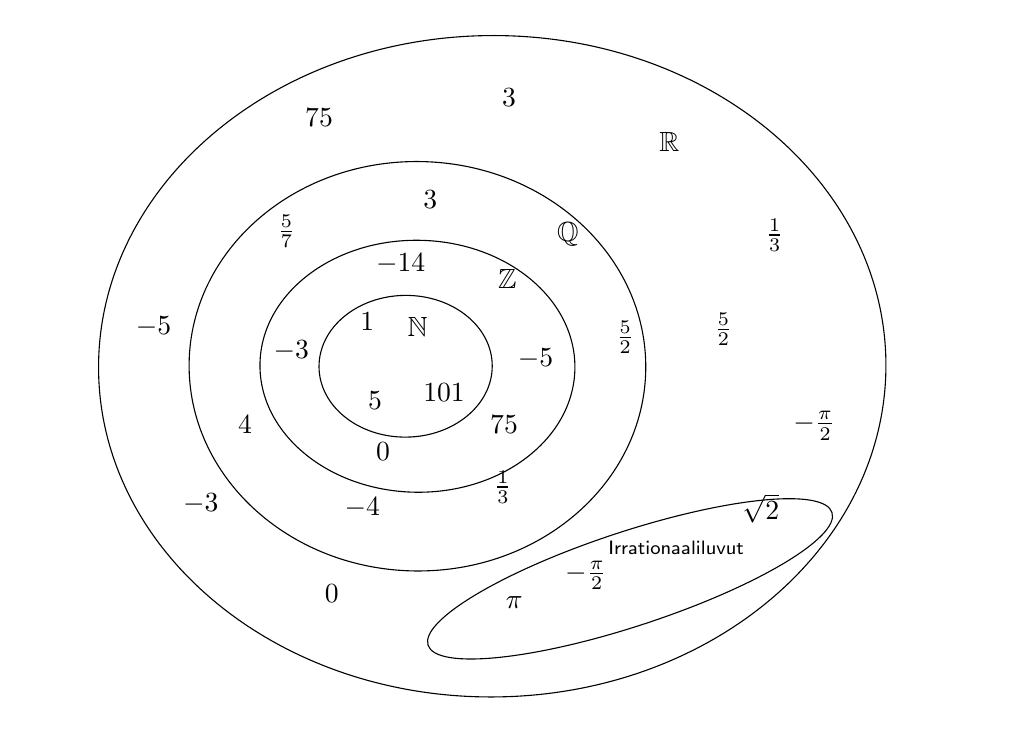
\begin{tikzpicture}[line cap=round,line join=round,>=triangle 45,x=0.5cm,y=0.5cm]
\clip(-7.4,-8.8) rectangle (16.8,8.6);
\draw [rotate around={0.5:(2.2,0)}] (2.2,0) ellipse (1.1cm and 0.9cm);
\draw [rotate around={-0.8:(2.5,0)}] (2.5,0) ellipse (2cm and 1.6cm);
\draw [rotate around={-0.8:(2.5,0)}] (2.5,0) ellipse (2.9cm and 2.6cm);
\draw (2,1.5) node[anchor=north west] {$\mathbb{N}$};
\draw (4.3,2.7) node[anchor=north west] {$\mathbb{Z}$};
\draw (5.8,3.9) node[anchor=north west] {$\mathbb{Q}$};
\draw (7.1,-4.2) node[anchor=north west] {{\scriptsize Irrationaaliluvut}}; %TODO: rotate
\draw (8.4,6.2) node[anchor=north west] {$\mathbb{R}$};
\draw [rotate around={0.5:(4.4,0)}] (4.4,0) ellipse (5cm and 4.2cm);
\draw [rotate around={18.2:(7.9,-5.4)}] (7.9,-5.4) ellipse (2.7cm and 0.6cm);
\draw (0.8,1.6) node[anchor=north west] {$1$};
\draw (1,-0.4) node[anchor=north west] {$5$};
\draw (2.4,-0.2) node[anchor=north west] {$101$};
\draw (4.8,0.7) node[anchor=north west] {$-5$};
\draw (1.2,-1.7) node[anchor=north west] {$0$};
\draw (1.2,3.1) node[anchor=north west] {$-14$};
\draw (4.1,-1) node[anchor=north west] {$75$};
\draw (4.2,-2.4) node[anchor=north west] {$\frac{1}{3}$};
\draw (7.3,1.4) node[anchor=north west] {$\frac{5}{2}$};
\draw (-1.4,0.9) node[anchor=north west] {$-3$};
\draw (0.4,-3.1) node[anchor=north west] {$-4$};
\draw (2.4,4.7) node[anchor=north west] {$3$};
\draw (-1.3,4.1) node[anchor=north west] {$\frac{5}{7}$};
\draw (-2.3,-1) node[anchor=north west] {$4$};
\draw (4.5,-5.6) node[anchor=north west] {$\pi$};
\draw (10.7,-3) node[anchor=north west] {$\sqrt[]{2}$};
\draw (6,-4.7) node[anchor=north west] {$-\frac{\pi}{2}$};
\draw (9.8,1.6) node[anchor=north west] {$\frac{5}{2}$};
\draw (11.1,4) node[anchor=north west] {$\frac{1}{3}$};
\draw (4.4,7.3) node[anchor=north west] {$3$};
\draw (-0.1,-5.3) node[anchor=north west] {$0$};
\draw (-4.9,1.5) node[anchor=north west] {$-5$};
\draw (11.8,-0.9) node[anchor=north west] {$-\frac{\pi}{2}$};
\draw (-0.6,6.8) node[anchor=north west] {$75$};
\draw (-3.7,-3) node[anchor=north west] {$-3$};
\end{tikzpicture}

Lukualueita voidaan laajentaa lisää vielä tästäkin, esimerkiksi \emph{imaginaariluvut} ovat lukuja, jotka eivät ole reaalilukuja, vaan lukuja, joita ei voi edes sijoittaa lukusuoralle. Reaalilukuja ja imaginaarilukuja kutsutaan yhdessä \emph{kompleksiluvuiksi}.

Kompleksilukuja tarvitaan mm. insinöörialoilla yliopistoissa ja ammattikorkeakouluissa. Esimerkiksi vaihtosähköpiirien analyysissä, signaalinkäsittelyssä ja säätötekniikassa käytetään runsaasti kompleksilukuja. Kompleksiluvut ovat tärkeitä myös matematiikan tutkimuksessa itsessään.

    \input{01-luvut/09-kertaus}

\part{Yhtälöt}
    \chapter{Yhtälö}

Monissa käytännön tilanteissa jokin suure voidaan päätellä tai laskea kahdella eri tavalla. Nämä tavat voidaan merkitä lukuina tai kirjoittaa lausekkeiksi. Merkitsemällä näin saadut lukuarvot ja lausekkeet yhtäsuuriksi saadaan \emph{yhtälö}. Yhtälö on siis kahden lausekkeen merkitty yhtäsuuruus. Yhtälöitä esiintyy usein käytännön tilanteissa.

\begin{esimerkki}
Merkitään lausekkeet $5x+\sqrt{x}$ ja $7x+7$ yhtäsuuriksi, jolloin saadaan
yhtälö $5x+\sqrt{x} = 7x+7$.
\end{esimerkki}

\laatikko{
Jos yhtälön kummankin puolen lausekkeen arvo on sama, sanotaan että \emph{yhtälö pätee}.
}

\begin{esimerkki}
\begin{enumerate}[a)]
\item Yhtälö $3x + 2 = 0$ pätee, kun $x = - \frac{2}{3}$.
\item Yhtälö $5 = 3$ ei päde.
\end{enumerate}
\end{esimerkki}


\begin{esimerkki}
Kuvassa oleva vaaka on tasapainossa. Toisessa vaakakupissa on kahden kilon siika ja toisessa puolen kilon ahven sekä tuntematon määrä lakritsia. Kuinka paljon vaakakupissa on lakritsia?
\todo{kahden kilon siika -esimerkin ratkaisu}
\missingfigure{Kuva kaloista vaa'assa}

\textbf{Ratkaisu.}

Merkitään lakritsin määrää tuntemattomalla $x$. Tilannetta kuvaa yhtälö
\begin{equation}
2 = 0{,5} + x.
\end{equation}

Ratkaistaan yhtälö.

\begin{align*}
2 &= 0{,5} + x &&\text{| $-0{,5}$} \\
2 - 0{,5} &= x && \\
1{,5} &= x && \\
x &= 1{,5} && \\
\end{align*}


\textbf{Vastaus.} Lakritsia on $1{,5}$ kg.
\end{esimerkki}

\todo{lisää yhtälöesimerkkejä}


\laatikko{
\begin{itemize}
\item Yhtälössä esiintyy yleensä \emph{tuntemattomia}, joiden arvoa ei tiedetä ja joita merkitään eri symboleilla. Jos tuntemattomia on vain yksi, sitä merkitään yleensä kirjaimella $x$.
\item Niitä tuntemattoman $x$ arvoja, joilla yhtälö pätee, kutsutaan yhtälön \emph{ratkaisuiksi}.
\item Yhtälön ratkaisemisella tarkoitetaan kaikkien yhtälön ratkaisujen selvittämistä.
\end{itemize}
}

\todo{jokin helposti ymmärrettävä esimerkki tuntemattomista}

\laatikko{
Tyypillinen tapa ratkaista yhtälöitä on kirjoittaa ne ilmaistuna toisella tavalla. Käytännössä se tarkoittaa sitä, että niitä muokkaa siten, ettei alkuperäisen yhtälön paikkansapitävyys muutu. Tällaisia sallittuja muunnoksia ovat esimerkiksi:
\begin{itemize}
\item Yhtälön molemmille puolille voidaan lisätä tai molemmilta puolilta voidaan vähentää luku. Esimerkiksi yhtälö $3x+5 = 3$ saadaan näin muotoon $3x = -2$.
\item Yhtälön molemmat puolet voidaan kertoa nollasta poikkeavalla luvulla.
Esimerkiksi kertomalla yhtälön $2x = 4$ molemmat puolet luvulla $\frac{1}{2}$
saadaan yhtälö $x = 2$.
\end{itemize}
}

Kuvitellaan orsivaaka, joka on tasapainossa. Vasemmalla ja oikealla puolella on eripainoisia esineitä, mutta ne painavat yhteensä yhtä paljon. Jos molemmille puolille lisätään nyt saman verran painoa, vaaka on yhä tasapainossa. Samalla tavalla yhtälön molemmille puolille on sallittua lisätä sama luku.

Yhtälöt ratkeavat siten, että niitä muokataan, kunnes vastauksen voi lukea siitä suoraan, esim $x=3$.
%Koska jokaisessa muokkausjonon yhtälössä ratkaisut ovat samat, näin saadaan %alkuperäisen yhtälön ratkaisut.

%%esimerkki tulee 1. asteen yhtälön yhteydessä

\laatikko{
Yhtälöitä on kolmenlaisia:
\begin{enumerate}
\item Yhtälö, joka on aina tosi. Esimerkiksi yhtälöt $8=8$ ja $x=x$.
\item Yhtälö, joka on joskus tosi. Esimerkiksi yhtälö $x+4=7$ on tosi, kun $x=3$,
ja epätosi muulloin.
\item Yhtälö, joka ei ole koskaan tosi. Esimerkiksi yhtälö $0=1$.
\end{enumerate}
}

Tärkeimpiä näistä ovat joskus todet yhtälöt.

\laatikko{Yleisiä yhtälönratkaisuperiaatteita:

\begin{itemize}
\item Kerro tuntematonta sisältävät lausekkeet pois nimittäjistä.
\item Yhdistä useat murtolausekkeet yhdeksi laventamalla.
\item Yhdistä tuntemattomat.
\item Kumoa juuret korottamalla yhtälö puolittain sopivaan potenssiin.
\item Sulkuja ei välttämättä aina kannata kertoa auki.
\item Yhtälö on ratkaistu vasta, kun jäljellä on enää vain yksi kappale tuntematonta suuretta, ja se sijaitsee yksin omalla puolellaan yhtälöä.


\end{itemize}
}

Siirrymme nyt tarkastelemaan tärkeää yhtälöiden lajia, ensimmäisen asteen yhtälöitä.

    \chapter{Ensimmäisen asteen yhtälö}

\laatikko{
Ensimmäisen asteen yhtälöksi kutsutaan yhtälöä, joka on esitettävissä muodossa $ax+b=0$, jossa $a \neq 0$.
}

Yhtälötyypin nimi tulee siitä, että korkein potenssi, johon tuntematon $x$
yhtälössä korotetaan, on $1$.

\begin{esimerkki}
Muun muassa seuraavat yhtälöt ovat ensimmäisen asteen yhtälöitä:
\begin{enumerate}[a)]
\item $2x = 4$
\item $5x+3 = 0$
\item $x+2 = 3x-4$
\end{enumerate}
\end{esimerkki}

\laatikko{
Ensimmäisen asteen yhtälö ratkaistaan siirtämällä ensin tuntemattoman $x$ sisältävät termit yhtälön vasemmalle puolelle ja vakiotermit oikealle puolelle. Tämän jälkeen yhtälö jaetaan puolittain tuntemattoman $x$ kertoimella.
}

\begin{esimerkki}
Yhtälön $7x+4=4x+7$ ratkaisu saadaan seuraavasti:
\begin{align*}
7x+4 &= 4x+7 & &| \, \text{Vähennetään molemmilta puolilta 4x.} \\
3x+4 &= 7 & &| \, \text{Vähennetään molemmilta puolilta 4.} \\
3x &= 3 & &| \, \text{Jaetaan molemmat puolet luvulla 3.} \\
x &= 1 & & \\
\end{align*}

\textbf{Vastaus.} $x=1$
\end{esimerkki}

Ensimmäisen asteen yhtälöllä on aina täsmälleen yksi ratkaisu.

\begin{theorem}
Kaikki muotoa $ax+b=cx+d$ olevat yhtälöt, joissa $a \neq c$, ovat ensimmäisen asteen yhtälöitä.
\end{theorem}

\begin{proof}
\begin{align*}
ax+b &= cx+d & &| \, \text{Vähennetään molemmilta puolilta $cx+d$}. \\
ax+b - (cx+d) &= 0 & &| \, \text{Järjestellään termejä uudelleen.} \\
ax - cx + b - d &= 0 & &| \, \text{Otetaan yhteinen tekijä.} \\
(a-c)x + (b-d) &= 0 & &
\end{align*}

Tämä on määritelmän mukainen ensimmäisen asteen yhtälö, koska $a \neq c$.
\end{proof}

\begin{esimerkki}
Yleinen lähestymistapa muotoa $ax+b = cx+d$ olevien yhtälöiden ratkaisuun: \\
(1) Vähennä molemmilta puolilta $cx$. Saat yhtälön $(a-c)x + b = d$. \\
(2) Vähennä molemmilta puolita $b$. Saat yhtälön $(a-c)x = d-b$. \\
(3) Jaa $(a-c)$:llä. Saat yhtälön ratkaistuun muotoon $x = \frac{d-b}{a-c}$.
\end{esimerkki}

\section*{Tehtäviä}

\begin{tehtava}
Mitä yhtälölle $ax+b = 0$ tapahtuu, jos kerroin $a$ saa arvon nolla?
Onko yhtälöllä ratkaisuja?
\begin{vastaus}
Jos $b = 0$, yhtälö toteutuu kaikilla $x$:n arvoilla. Jos $b \neq 0$, yhtälö
ei toteudu millään $x$:n arvolla. Periaatteessa kyseessä ei kuitenkaan
enää ole ensimmäisen asteen yhtälö, mikäli $a = 0$
\end{vastaus}
\end{tehtava}

\begin{tehtava}
%
Ratkaise:
\begin{enumerate}[a)]
\item $x + 4 = 5$
\item $1 - x = -3$
\item $7x = 35$
\item $-2x = 4$
\item $10 - 2x = x$
\item $9x + 4 = 6 - x$
\item $\frac{2x}{5} = 4$
\item $\frac{x}{3} + 1 = \frac{5}{6} - x$
\end{enumerate}
\begin{vastaus}
\begin{enumerate}[a)]
\item $x=1$
\item $x=4$
\item $x=35/7$
\item $x=-2$
\item $x=10/3$
\item $x=1/5$
\item $x=10$
\item $x=-1/8$
\end{enumerate}
\end{vastaus}
\end{tehtava}

\begin{tehtava}
Ratkaise kysytty tuntematon yhtälöstä
\begin{enumerate}[a)]
\item $F=ma$, $m=?$ (Voima on massa kerrottuna kiihtyvyydellä.)
\item $p=\frac{F}{A}$, $F=?$ (Paine on voima jaettuna alalla.)
\item $A=\pi r^2$, $r=?$ (Ympyrän pinta-ala on pii kerrottuna säteen neliöllä.)
\item $V=\frac{1}{3} \pi r^2 h$, $h=?$ (Kartion tilavuus on piin kolmasosa
kerrottuna säteen neliöllä ja kartion korkeudella.)
\end{enumerate}
\begin{vastaus}
\begin{enumerate}[a)]
\item $m=\frac{F}{a}$
\item $F=p A$
\item $r=\sqrt{\frac{A}{\pi}}$
\item $h=\frac{V}{ \frac{1}{3} \pi r^2 h}$
\end{enumerate}
\end{vastaus}
\end{tehtava}

\begin{tehtava}
Kännykkäliittymän kuukausittainen perusmaksu on 2,90 euroa. Lisäksi jokainen puheminuutti ja tekstiviesti maksaa 0,69 senttiä. Pekan kännykkälasku kuukauden
ajalta oli 27,05 euroa.

\begin{enumerate}[a)]
	\item Kuinka monta puheminuuttia/tekstiviestiä Pekka käytti kuukauden aikana?
	\item Pekka lähetti kaksi tekstiviestiä jokaista viittä puheminuuttia kohden. Kuinka monta tekstiviestiä Pekka lähetti?
\end{enumerate}

	\begin{vastaus}
		\begin{enumerate}[a)]
			\item 350 puheminuuttia/tekstiviestiä
			\item 100 tekstiviestiä
		\end{enumerate}
	\end{vastaus}
\end{tehtava}

\begin{tehtava}
Sadevesikeräin näyttää vesipatsaan korkeuden millimetreinä. Eräänä aamuna
keräimessä oli 5 mm vettä. Seuraavana aamuna samaan aikaan keräimessä oli 23 mm vettä. Muodosta yhtälö ja selvitä, kuinka paljon vettä oli keskimäärin satanut kuluneen vuorokauden aikana tunnissa.
	\begin{vastaus}
	$0,75$ mm/tunti
	\end{vastaus}
\end{tehtava}

    \chapter{Prosenttilaskenta}

Sana prosentti tulee latinan kielen sanoista pro centum, mikä tarkoittaa kirjaimellisesti sataa kohden. Prosentteja käytetään ilmaisemaan suhteellista osuutta. Prosentin merkki on \%.


\laatikko{1 prosentti $= 1\ \% = \frac{1}{100} = 0,01$}

\begin{esimerkki}
\mbox{}
\begin{itemize}
	\item $6 \ \% = \frac{6}{100} = 0,06$
	\item $48,2 \ \% = \frac{48,2}{100} = 0,482$
	\item $140 \ \% = \frac{140}{100} = 1,40$
\end{itemize}
\end{esimerkki}

\todo{tehtävä: ilmaise desimaalilukuna seuraavat prosentit}

%%%%PERUSARVO%%%%%%%
\laatikko{
Lukua, josta suhde lasketaan, kutsutaan \emph{perusarvoksi}.
}


\begin{esimerkki}
Jos sadan euron hintaisen tuotteen hintaa on alennettu 25 prosenttia, niin alennettu hinta on 75 euroa. Jos sen sijaan alkuperäinen hinta nousee 15 prosenttia, niin tuotteen uusi hinta on 115 euroa. Perusarvo on molemmissa tapauksissa 100 euroa.

\missingfigure{kuva suorakaiteesta, joka kuvaa perusarvoa (se voi olla vaik 10x10 pientä laatikkoa. Sit kuva, jossa peruarvosta on vähennetty 25~\% perusarvosta, eli 75 laatikkoa. Sit kuva, jossa perusarvoon on lisätty 15~\%, eli 115 laatikkoa. Sit sopivat havainnollistavat väritykset}
\end{esimerkki}


\todo{tehtävä perusarvosta}


%MUUTOSPROSENTTITEORIA
\laatikko{
Prosentteja käytetään usein ilmaisemaan suureiden muutoksia, esimerkiksi luku $b$ kasvaa luvuksi $a$. \emph{Muutosprosenttia} laskettaessa muutoksen suuruttaa verrataan alkuperäiseen lukuun. Perusarvona on siis alkuperäinen arvo, johon nähden muutos on tapahtunut.

Jos kysytään, kuinka monta prosenttia $a$ on isompi $b$:tä, se tarkoittaa samaa, kuin kuinka monta $b$:n sadasosaa on se määrä, jolla $a$ on suurempi $b$:tä. Toisin sanoen kuinka monta $b$:n sadasosaa mahtuu $a-b$:hen. Se saadaan laskemalla

\begin{equation*}
\frac{a-b}{\frac{b}{100}} = \frac{a-b}{b} \cdot 100
\end{equation*}

Samalla tavalla saadaan laskettua, kuinka monta prosenttia luku kasvoi, kun se muuttui $a$:sta $b$:hen.
}




%TÄMÄ ON MUUTOSPROSENTTITEHTÄVÄESIMERKKI
\begin{esimerkki}
Vesan paino on tammikuussa 68 kg ja kesäkuussa 64 kg. Kuinka monta prosenttia Vesa on laihtunut?

\textbf{Ratkaisu.}

Lasketaan 
\begin{equation*}
\frac{68-64}{68}\cdot 100\ \% = \frac{4}{68} \cdot 100\ \%=0,06\cdot 100\ \% = 6\ \%
\end{equation*}

\textbf{Vastaus.}

Vesa on laihtunut $6\ \%$.
\end{esimerkki}


\todo{alv-tehtävä}
\includegraphics[width=80mm, angle=270]{02-yhtalot/kuvia/alv-kuitti}

%%%VERTAILUPROSENTTI%%%%%
\laatikko{
\emph{Vertailuprosentilla} ilmaistaan, kuinka monta prosenttia luku on jostain toisesta luvusta. Vertailuprosentin laskennassa käytetään perusarvona sitä lukua, johon verrataan.

Jos kysytään, kuinka monta prosenttia $b$ on $a$:stä, se tarkoittaa samaa, kuin kuinka monta $a$:n sadasosaa $b$ on. Toisin sanoen kuinka monta $a$:n sadasosaa $b$:hen mahtuu. Se saadaan laskemalla 

\begin{equation*}
\frac{b}{\frac{a}{100}} = \frac{b}{a} \cdot 100
\end{equation*}

\missingfigure{havainnollistava kuva vertailuprosentista suorakulmioiden avulla}
}

%TÄMÄ ON VERTAILUPROSENTTITEHTÄVÄESIMERKKI
\begin{esimerkki}
Vesa ansaitsee kuukaudessa ${2\,300}$ euroa ja Antero ${1\,700}$ euroa. Kuinka monta prosenttia Anteron tulot ovat Vesan tuloista? 

\textbf{Ratkaisu.}

Lasketaan

\begin{equation*}
\frac{1700}{2300} \cdot 100\ \%  \approx 0,74\cdot 100\ \% = 74 \  \%.
\end{equation*}

Laskuissa käytettävä perusarvo on Vesan palkka eli 2300 euroa.
    
\textbf{Vastaus.}

$74~\%$
\end{esimerkki}



%%%%PROSENTTIYKSIKKÖ
\laatikko{
\emph{Prosenttiyksikkö} mittaa prosenttiosuuksien välisiä eroja. Esimerkiksi $4\ \%$ on $2$ prosenttiyksikköä suurempi kuin $2\ \%$, mutta $100\ \%$ suurempi kuin $2\ \%$. Jos prosenttiluku muuttuu, muutos voidaan ilmaista joko prosentteina tai prosenttiyksikköinä.
}


%%%%%%PROSENTTIYKSIKKÖTEHTÄVÄESIMERKKI
\begin{esimerkki}
    Tuotteen markkinaosuus on vuoden tammikuussa 10~\% ja kesäkuussa 15~\%. 
    \begin{enumerate}[a)]
    \item Kuinka monta prosenttia tuotteen markkinaosuus on noussut?
    
    \item Kuinka monta prosenttiyksikköä tuotteen markkinaosuus on noussut?
    \end{enumerate}
    
    {\bf Ratkaisu.} 
    
    \begin{enumerate}[a)]
    \item Tuotteen markkinaosuus on noussut
    \[
    \frac{15-10}{10} \cdot 100\ \%= \frac{5}{10}\cdot 100\ \% = 50\ \%.
    \]
    
    \item Tuotteen markkinaosuus on noussut $15-10=5$ prosenttiyksikköä. 
    \end{enumerate}
    
    {\bf Vastaus.}
    
    \begin{enumerate}[a)]
    \item 50 prosenttia
    \item 5 prosenttiyksíkköä.
    \end{enumerate}
\end{esimerkki}

\section*{Tehtäviä}

\begin{tehtava}
    Laukun normaalihinta on 225 euroa, ja se on 25~\%:n alennuksessa.
    Mikä on alennettu hinta?
    \begin{vastaus}
    Vastaus: 168,75 euroa
    \end{vastaus}
\end{tehtava}

\begin{tehtava}
    Jaakon kuukausipalkka on 1623,52 euroa. Hän saa 1,3\, \% palkankorotuksen.
    Mikä on Jaakon kuukausipalkka korotuksen jälkeen?
    \begin{vastaus}
    1644,63 euroa
    \end{vastaus}
\end{tehtava}

\begin{tehtava}
    %Pyramidi 1, s. 80
    Kirjan myyntihinta, joka sisältää arvolisäveron, on 8~\% suurempi kuin kirjan veroton hinta. Laske kirjan veroton hinta, kun myyntihinta on 15 euroa.
    \begin{vastaus}
        Vastaus: Kirjan veroton hinta on 13,89 euroa
    \end{vastaus}
\end{tehtava}

\begin{tehtava}
    Perussuomalaisten kannatus oli vuoden 2007 eduskuntavaaleissa 4,1~\% ja vuoden 2011 eduskuntavaaleissa 19,1~\%. Kuinka monta prosenttiyksikköä kannatus nousi? Kuinka monta prosenttia kannatus nousi?
    \begin{vastaus}
    Vastaus: Kannatus nousi 15 prosenttiyksikköä. Prosentteina mitattuna kannatus nousi 366~\%.
    \end{vastaus}
\end{tehtava}

\begin{tehtava}
    Askartelukaupassa on alennusviikot, ja kaikki tavarat myydään 60~\%:n alennuksella. Viimeisenä päivänä kaikista hinnoista annetaan vielä lisäalennus, joka lasketaan aiemmin alennetusta hinnasta. Minkä suuruinen lisäalennus tulee antaa, jos lopullisen kokonaisalennuksen halutaan olevan 80~\%?
    \begin{vastaus}
        Vastaus: 50~\%.
    \end{vastaus}
\end{tehtava}

\begin{tehtava}
    Erään pankin myöntämä opintolaina kasvaa korkoa 2~\% vuodessa. Kuinka monta prosenttia laina on kasvanut korkoa alkuperäiseen verrattuna kymmenen vuoden kuluttua?
    \begin{vastaus}
        Vastaus: 22~\%.
    \end{vastaus}
\end{tehtava}

\begin{tehtava}
Yleinen arvonlisäveroprosentti oli Suomessa vuonna 2012 23~\% tuotteen verottomasta
hinnasta. Tuotteen hinta koostuu sen verottomasta hinnasta
ja tuotteesta maksettavasta arvonlisäverosta. Kuinka monta
prosenttia arvonlisävero on tuotteen myyntihinnasta?
\begin{vastaus}
18,0~\%
\end{vastaus}
\end{tehtava}

%Ansiotuloverotus on Suomessa progressiivista: suuremmista tuloista maksetaan

\begin{tehtava}
    Tuoreissa omenissa on vettä 80~\% ja sokeria 4~\%. Kuinka monta prosenttia sokeria on samoissa omenissa, kun ne on kuivattu siten, että kosteusprosentti on 20? [K2000, 4]
    \begin{vastaus}
        Vastaus: 16~\%
    \end{vastaus}
\end{tehtava}

\begin{tehtava}
    Kappaleen putoamisen kesto maahan korkeudelta $x$ on kääntäen verrannollinen putoamiskiihtyvyyden $g$ neliöjuureen. Vakio $g$ on kullekin taivaankappaleelle ominainen ja eri puolilla taivaankappaletta likimain sama. Empire State Buildingin katolta (korkeus $381$ m) pudotetulla kuulalla kestää n. $6,2$ s osua maahan. Marsin putoamiskiihtyvyys on $37,6$ \% Maan putoamiskiihtyvyydestä. 
    
    Jos Empire State Building sijaitsisi Marsissa, kuinka monta prosenttia pitempi aika kuluisi kuulan maahan osumiseen?
    \begin{vastaus}
        Vastaus: $10$ s
    \end{vastaus}
\end{tehtava}

\begin{tehtava}
Matin ja Iidan duo saa julkisuutta, ja he alkavat myydä CD-levyään keikkojen yhteydessä 10 euron kappalehinnalla. Jonkin ajan päästä he päättävät laskea CD:n hintaa 20 prosenttia. Matti alkaa kuitenkin katua päätöstä, ja ehdottaa tämän alennetun hinnan korottamista 20 prosentilla. Mikä olisi tämän toimenpiteen jälkeen CD:n uusi hinta? Montako prosenttia olisi korotuksen oltava, jotta oikeasti päästäisiin takaisin alkuperäiseen 10 euron hintaan?
    \begin{vastaus}
25~\%
    \end{vastaus}
\end{tehtava}

\begin{tehtava}
(YO 1877 4) Kaupungissa tuli jokaisen talonomistajan suorittaa kaupungin kassaan 5~\% saadusta hyyrymäärästä. Sittemmin määrättiin, että mainittu prosentti oli oleva 10. Monellako prosentilla täytyy talonomistajien korottaa hyyryjä saadakseen saman puhtaan säästön kuin ennen? 
    \begin{vastaus}
5,6~\%
    \end{vastaus}
\end{tehtava}

    \input{02-yhtalot/05-potenssiyhtalot}
    \input{02-yhtalot/06-kertaus}

\part{Funktiot}
    \chapter{Funktio}

Usein ollaan kiinnostuneita siitä, millainen yhteys kahden asian välillä
on. Funktio on matemaattinen työkalu näiden yhteyksien tarkastelemiseen.

\laatikko{
\emph{Funktio} $f$ liittää \emph{muuttujaan} $x$ arvon $f(x)$.

Funktiolla on \emph{määrittelyjoukko} $A$, johon muuttuja $x$ kuuluu, ja \emph{maalijoukko} $B$, johon funktion arvot kuuluvat.
}

\begin{esimerkki}
Hyödykkeen ja siitä maksettavan arvonlisäveron välistä yhteyttä
voidaan kuvata funktiolla. Valitaan funktion määrittelyjoukoksi
tiettyjen hyödykkeiden joukko,
\[
A = \{\text{ahvenfilee}, \text{AIV-rehu}, \text{auto}, \text{runokirja}, \text{ravintola-ateria}, \text{särkylääke}, \text{televisio}\},
\]
ja arvojoukoksi reaaliluvut. Funktio voi liittää kuhunkin hyödykkeeseen
esimerkiksi siitä maksettavan arvonlisäveroprosentin:
$f(\text{särkylääke}) = 9$ ja $f(\text{televisio}) = 23$.

\begin{center}
\includegraphics[width=13cm]{03-funktiot/kuvia/funktiokone.pdf}
\end{center}
\end{esimerkki}

Funktioiden käyttämiseen liittyy joitakin vakiintuneita tapoja:
\begin{itemize}
\item $f(x) = y$ lausutaan: ''Funktio saa arvon $y$ pisteessä $x$'',
\item Funktion määrittely- ja arvojoukko jätetään usein merkitsemättä, jos ne voidaan päätellä asiayhteydestä. Tällä kurssilla arvojoukkona on yleensä reaaliluvut.
\item Toisinaan funktiolle ja funktion kuvaajalle ei tehdä selkeää eroa:
$y = f(x)$ samaistetaan koordinaatistoon piirretyn funktion kuvaajan kanssa.
Periaatteessa funktio ja sen kuvaaja ovat kuitenkin eri asioita.
\end{itemize}

Funktiolla on usein jokin selkeä sääntö, joka voidaan kirjoittaa
matemaattisena lausekkeena.

\begin{esimerkki}
Jos neliön sivun pituutta merkitään $x$:llä, voidaan sivun pituuden
ja neliön pinta-alan välistä yhteyttä kuvata funktiolla
$A(x) = x^2$.
\end{esimerkki}

Funktion määrittelyjoukko koostuu niistä muuttujan arvoista, joilla
funktio on määritelty eli joilla funktion arvo voidaan laskea.

\begin{esimerkki}
Määritellään funktio $f$ lausekkeella
\[
f(x) = \frac{1}{x-1}.
\]
Mikä on funktion määrittelyjoukko?

\textbf{Ratkaisu.}
Funktio $f(x)$ on määritelty, kun nimittäjä $x-1$ on erisuuri
kuin 0. Tämä toteutuu kaikilla $x$:n arvoilla lukuun ottamatta
arvoa $x = 1$. Funktion määrittelyjoukkoon kuuluvat siis
kaikki reaaliluvut paitsi luku 1.
\end{esimerkki}

Funktion \emph{arvojoukko} sisältää ne maalijoukon alkiot,
jotka funktio saa arvokseen ainakin yhdessä pisteessä.

\esimerkki{
Mikä on edellä määritellyn funktion $f(x)$ arvojoukko?

\textbf{Ratkaisu.}
Arvojoukon selvittämiseksi tutkitaan, millä luvun $a$ arvoilla
yhtälöllä $f(x) = a$ on ratkaisu,
\begin{align*}
a &= \frac{1}{x-1} & &| \, \text{Oletetaan, että $x \neq 1$, jolloin voimme kertoa $(x-1)$:llä puolittain.} \\
a(x-1) &= 1 \\
x-1 &= \frac{1}{a} \\
x &= 1+\frac{1}{a} & &| \, \text{Havaitaan, että yhtälöllä on ratkaisu
kaikilla $a \neq 0$.}
\end{align*}
Funktion arvojoukkona on siis koko reaalilukujen joukko.
}


\section*{Tehtäviä}
\begin{tehtava}
Olkoon $f(x)=\frac{2^x+4}{x}$. Laske
\begin{enumerate}[a)]
\item $f(1)$
\item $f(2)$
\item $f(\frac{1}{2})$
\item $f(\frac{1}{3})$
\item $f(0)$
\item $f(-1)$
\end{enumerate}
\begin{vastaus}
\begin{enumerate}[a)]
\item $6$
\item $4$
\item $2\sqrt{2}+8$
\item $3\sqrt[3]{2}+12$
\item ei määritelty
\item $\frac{-9}{2}$
\end{enumerate}
\end{vastaus}
\end{tehtava}

% kai vaikeahko
\begin{tehtava}
Millä $x$:n arvoilla yhtälö $f(f(x)) = x$ pätee, kun
\begin{enumerate}[a)]
\item $f(x) = 1$
\item $f(x) = x$
\item $f(x) = x+1$
\item $f(x) = 2x$
\item $f(x) = 2x+1$?
\end{enumerate}

\begin{vastaus}
\begin{enumerate}[a)]
\item $x = 1$
\item kaikilla $x\in\mathbb{R}$
\item ei ratkaisuja
\item $x = 0$
\item $x = -1$
\end{enumerate}
\end{vastaus}
\end{tehtava}

    \chapter{Koordinaatisto ja funktion kuvaaja}
Funktioita reaaliluvuilta reaaliluvuille voidaan havainnollistaa koordinaatistossa kuvaajien avulla. Funktion $f$ kuvaajassa koordinaatistoon piirretään ne pisteet, joilla y-koordinaatti on $f$:n arvo sen x-koordinaatissa. Siis kaikilla $f$:n määrittelyjoukon luvuilla $x$ lasketaan $y = f(x)$ ja piirretään piste $(x, y)$ koordinaatistoon. Funktioita voi piirtää helposti myös graafisilla laskimilla tai tietokoneohjelmilla (esimerkiksi Wolfram Alphalla\footnote{http://www.wolframalpha.com}).

% Tarvitaan kuvien ja taulukkojen vierekkäin laittamiseen.
\def\vcent#1{\mathsurround0pt$\vcenter{\hbox{#1}}$}

\begin{esimerkki}
Funktion $f(x) = \frac{x}{2} - 1$ kuvaaja sisältää kaikki pisteet $(x, y)$, joilla pätee $y = \frac{x}{2} - 1$:
\begin{center}
\begin{tabular}{cc}
\begin{tabular}{|r|l|}
\hline
$x$ & $y = f(x)$ \\
\hline
$-3$ & $-2,5$ \\
$-2$ & $-2$ \\
$-1$ & $-1,5$ \\
$0$ & $-1$ \\
$1$ & $-0,5$ \\
$2$ & $0$ \\
$3$ & $0,5$ \\
\hline
\end{tabular} &
\vcent{\includegraphics[width=8cm]{03-funktiot/kuvia/suoraesim.pdf}}
\end{tabular}
\end{center}
\end{esimerkki}

\begin{esimerkki}
Funktion $f(x) = x^2$ kuvaaja sisältää kaikki pisteet $(x, y)$, joilla pätee $y = x^2$:
\begin{center}
\begin{tabular}{cc}
\begin{tabular}{|r|l|}
\hline
$x$ & $y = f(x)$ \\
\hline
$-2$ & $4$ \\
$-1$ & $1$ \\
$-0,5$ & $0.25$ \\
$0$ & $0$ \\
$0,5$ & $0.25$ \\
$1$ & $1$ \\
$2$ & $4$ \\
\hline
\end{tabular} &
\vcent{\includegraphics[width=6cm]{03-funktiot/kuvia/paraabeli.pdf}}
\end{tabular}
\end{center}
\end{esimerkki}

\begin{esimerkki}
Funktion $f(x) = x^3-5x+2$ kuvaaja sisältää kaikki pisteet $(x, y)$, joilla pätee $y = x^3-5x+2$:
\begin{center}
\includegraphics[width=7cm]{03-funktiot/kuvia/deg3polynomiesim.pdf}
\end{center}
\end{esimerkki}

\section*{Tehtäviä}

\subsubsection*{Opi perusteet}

\begin{tehtava}
Hahmottele funktion kuvaaja kynällä ja paperilla tai laskimen avulla. Voit myös käyttää tietokonetta.
\begin{enumerate}[a)]
\item $f(x) = 2$
\item $f(x) = 3x+2$
\item $f(x) = x^2$
\item $f(x) = \frac{2}{x}$
\end{enumerate}

%\begin{vastaus}
%\end{vastaus}
\end{tehtava}

    \chapter{Suoraan ja kääntäen verrannollisuus}

Kaksi muuttujaa voivat riippua toisistaan monin eri tavoin. Tavallisia
riippuvuuden tyyppejä ovat suoraan ja kääntäen verrannollisuus.

\laatikko{
Kaksi muuttujaa $x$ ja $y$ ovat suoraan verrannolliset, jos toinen saadaan
toisesta kertomalla se jollakin vakiolla, eli $y = kx$. Vakiota $k$
kutsutaan \emph{verrannollisuuskertoimeksi}.}

Jos suureet $x$ ja $y$ ovat suoraan verrannolliset, niin tätä merkitään $x\sim y$ tai $x\propto y$.

Suoraan verrannollisuus voidaan tunnistaa esimerkiksi laskemalla muuttujien
suhde ja toteamalla, että se on muuttujista riippumaton vakio.

\begin{esimerkki}
Banaanien kilohinta on $2,00$ euroa. Seuraavassa taulukossa on
banaanien paino\footnote{Fysikaalisesti kyse on massasta, mutta
arkikielessä käytetään sanaa paino.}, jonka saa ostettua tietyllä rahamäärällä:
\begin{center} 
\begin{tabular}{|l|r|r|}
\hline
Hinta (euroa) & Paino (kg) & Hinta/paino (euroa/kg) \\
\hline
$1,00$ & $0,50$ & $2,00$ \\
$2,00$ & $1,00$ & $2,00$ \\
$3,00$ & $1,50$ & $2,00$ \\
$4,00$ & $2,00$ & $2,00$ \\
\hline
\end{tabular}
\end{center}
Hinnan ja painon suhde on vakio, $2,00$ euroa/kg, joten ostettujen
banaanien paino ja niihin käytetty rahamäärä ovat suoraan verrannolliset.
\end{esimerkki}

Suoraan verrannollisuutta voidaan kuvata myös niin, että jos
toinen muuttujista kaksinkertaistuu, niin toinenkin kaksinkertaistuu.
Samoin jos toisen muuttujan arvo puolittuu, toisenkin arvo puolittuu.

Jos suoraan verrannollisista muuttujista piirretään kuvaaja, pisteet
asettuvat suoralle:

\missingfigure{Kuva, johon piirretty vaaka-akselille käytetty rahamäärä
ja pystyakselille ostettujen banaanien paino.}

Suoraan verrannollisia muuttujia ovat myös esimerkiksi
\begin{itemize}
    \item aika ja kuljettu matka, kun liikutaan vakionopeudella, tai
    \item kappaleen massa ja painovoiman kappaleeseen aiheuttama voima.
\end{itemize}

Suoraan verrannollisuutta monimutkaisempi riippuvuus on kääntäen
verrannollisuus.

\laatikko{
Muuttujat $x$ ja $y$ ovat kääntäen verrannolliset, jos toinen saadaan toisesta
jakamalla jokin vakio sillä, eli $y = \frac{a}{x}$.
}

Kääntäen verrannollisuus voidaan tunnistaa esimerkiksi
kertomalla muuttujien arvoja keskenään ja huomaamalla,
että tulo on muuttujista riippumaton vakio.

\begin{esimerkki}
Nopeus ja matkaan tarvittava aika ovat kääntäen verrannolliset.
Jos kuljettavana matkana on $80$ km, voidaan nopeudet ja matka-ajat
kirjoittaa taulukoksi:
\begin{center} 
\begin{tabular}{|l|r|r|}
\hline
Nopeus (km/h) & Matka-aika (h) & Nopeus$\cdot$matka-aika (km) \\
\hline
$40$ & $2$ & $80$ \\
$80$ & $1$ & $80$ \\
$100$ & $0,8$ & $80$ \\
\hline
\end{tabular}
\end{center}
Tulo on aina $80$ km, joten nopeus ja matka-aika ovat kääntäen verrannolliset.
\end{esimerkki}

Kääntäen verrannollisuutta voidaan kuvata myös niin, että jos
toinen muuttujista kaksinkertaistuu, toinen puolittuu.

Jos kääntäen verrannollisista muuttujista piirretään kuvaaja, pisteet
muodostavat laskevan käyrän:

\missingfigure{Kuva, johon on piirretty matka-aika ja nopeus (yllä olevan
taulukon mukaisesti).}

Kääntäen verrannollisia muuttujia ovat myös esimerkiksi
\begin{itemize}
    \item kaivamistyön suorittamiseen kuluva aika ja työntekijöiden lukumäärä.
\end{itemize}

\section*{Tehtäviä}

\begin{tehtava}
    % Lyhyt matikka 1, s. 72
    Pohdi seuraavissa tapauksissa, kuinka toinen muuttuja muuttuu, kun toinen
    kaksinkertaistuu, kolminkertaistuu tai puolittuu. Ovatko muuttujat
    suoraan verrannolliset, kääntäen verrannolliset vai eivät kumpaakaan?
    
    \begin{enumerate}
        \item Kuljettu matka ja kulunut aika, kun keskinopeus on 30 km/h.
        \item Kananmunien lukumäärä ja niiden kovaksi keittämiseen tarvittava keittoaika.
        \item Hedelmätiskiltä valitun vesimelonin paino ja hinta.
        \item Neliön sivun pituus ja neliön pinta-ala.
    \end{enumerate}
    
    \begin{vastaus}
        Vastaus:
        \begin{enumerate}
            \item Ovat.
            \item Eivät ole.
            \item Ovat.
            \item Eivät ole, sillä esimerkiksi kun neliön sivun pituus
                kaksinkertaistuu 1 cm:stä 2 cm:iin, niin neliön pinta-ala
                nelinkertaistuu 1 cm$^2$:stä 4 cm$^2$:iin.
        \end{enumerate}
    \end{vastaus}
\end{tehtava}

\begin{tehtava}
Ratkaise
\begin{enumerate}
\item $ \frac{x}{3} = 1$
\item $ \frac{8}{x} = 2$
\item $ \frac{7}{x} = \frac{16}{8}$
\item $ \frac{x}{3} = \frac{1}{7}$
\end{enumerate}
\begin{vastaus}
\begin{enumerate}
\item $x= \frac{1}{3}$
\item $y= \frac{1}{4}$
\item $x= \frac{7}{2}$
\item $x= \frac{3}{7}$
\end{enumerate}
\end{vastaus}
\end{tehtava}

\begin{tehtava}
Muodosta seuraavia tilanteita kuvaavat yhtälöt. Voit käyttää vakion
merkkinä esimerkiksi $c$:tä.
\begin{enumerate}
\item Kultakimpaleen arvo ($x$) on suoraan verrannollinen sen massaan ($m$),
eli mitä painavampi kimpale on, sitä enemmän siitä saa rahaa.
\item Aidan maalaamiseen osallistuvien ihmisten määrä {$x$} on kääntäen verrannollinen maalaamiseen kuluvaan aikaan ($t$). Toisin sanoen, mitä
enemmän maalaajia, sitä nopeammin homma on valmis.
\item Planeettojen toisiinsa aiheuttama vetovoima ($F$) on suoraan verrannollinen planeettojen massoihin ($m_1$ ja $m_2$) ja kääntäen verrannollinen niiden välisen etäisyyden ($r$) neliöön.
\end{enumerate}
\begin{vastaus}
\begin{enumerate}
\item $ \frac{x}{m}=c$
\item $ xt=c $
\item $ \frac{Fr^2}{m_1+m_2}=c$
\end{enumerate}
\end{vastaus}
\end{tehtava}

\begin{tehtava}
Rento pyöräilyvauhti kaupunkiolosuhteissa on noin $20$ km/h. Lukiolta urheiluhallille on matkaa $7$ km. Kuinka monta minuuttia kestää arviolta pyöräillä lukiolta urheiluhallille?
\begin{vastaus}
Viiden minuutin tarkkuudella $20$ min.
\end{vastaus}
\end{tehtava}

\begin{tehtava}
    Isä ja lapset ovat ajamassa mökille Sotkamoon. On ajettu jo neljä
    viidesosaa matkasta, ja aikaa on kulunut kaksi tuntia. ``Joko ollaan perillä?''
    lapset kysyvät takapenkiltä. Kuinka pitkään vielä arviolta kuluu, ennen
    kuin ollaan mökillä?
    
    \begin{vastaus}
        Vastaus: 1 h 15 min
    \end{vastaus}
\end{tehtava}

\begin{tehtava}
    Äidinkielen kurssilla annettiin tehtäväksi lukea 300-sivuinen romaani.
    Eräs opiskelija otti aikaa ja selvitti lukevansa vartissa seitsemän sivua.
    Kuinka monta tuntia häneltä kuluu koko romaanin lukemiseen, jos
    taukoja ei lasketa?
    
    \begin{vastaus}
        Vastaus: 642 minuuttia eli 10 h 42 min.
    \end{vastaus}
\end{tehtava}

    \input{03-funktiot/03-potenssifunktio}
    \chapter{Eksponenttifunktio}

Potenssifunktiossa $f(x) = x^n$ muuttuja $x$ on kantalukuna. Jos muuttuja
$x$ on sen sijaan eksponenttina, saadaan joukko funktioita, joita
kutsutaan \emph{eksponenttifunktioiksi}.

\laatikko{Eksponenttifunktiot ovat muotoa $f(x) = a^x$, $a > 0$,
$a \neq 1$ olevia funktioita.}

Eksponenttifunktioita on kahta tyyppiä: kasvavia ja väheneviä.
Kasvavilla eksponenttifunktioilla $a>1$, esimerkiksi

\begin{center}
\includegraphics{03-funktiot/kuvia/apotenssiinxaisompikuinyksi.pdf}
\end{center}

Vähenevillä eksponenttifunktioilla $0<a<1$, esimerkiksi

\begin{center}
\includegraphics{03-funktiot/kuvia/apotenssiinxaisompikuinnolla.pdf}
\end{center}

Negatiiviselle kantaluvulle ei ole määritelty yleistä reaalilukupotenssia, 
joten eksponenttifunktiota ei ole määritelty, kun $a < 0$. 

Kun $a=0$ tai $a=1$, eksponenttifunktio pelkistyy vakiofunktioksi.
Lisäksi $0^0$:a ei ole määritelty, joten vaaditaan, että
eksponenttifunktion kantaluvulle $a$ pätee $a>0$ ja $a \neq 1$.

%\emph{Eksponenttiyhtälö} muodostuu, kun kysytään, millä $x$:n arvoilla %eksponenttifunktio saavuttaa tietyn arvon.

\begin{esimerkki}
Millä muuttujan $x$ arvoilla eksponenttifunktio $f(x) = 2^x$ saa arvon
$f(x) = 64$?

\textbf{Ratkaisu.}
Kirjoitetaan tehtävä yhtälöksi: $2^x = 64$. Kokeilemalla huomataan,
että $x = 6$ ratkaisee yhtälön.

Varmistutaan vielä siitä, että yhtälöllä ei ole muita ratkaisuja.
Eksponenttifunktion kantalukuna on $2$, joten eksponenttifunktio on
kasvava. Funktio $f(x) = 2^x$ ei siis voi saada uudelleen arvoa $64$,
kun $x > 6$. Samasta syystä $f(x)$ ei voi olla $64$, kun $x < 6$.

Ainoa ratkaisu yhtälölle on siis $x = 6$.
\end{esimerkki}

\begin{esimerkki}
Millä muuttujan $x$ arvoilla eksponenttifunktio
$f(x) = \left( \frac{1}{2} \right)^{x}$ saa arvon
$f(x) = 1/5$?

\textbf{Ratkaisu.}
Edellisen esimerkin tavoin kokeillaan $x$:n eri arvoja. Havaitaan,
että kun $x = 2$, funktio saa arvon $f(x) = \frac{1}{4}$, ja
kun $x = 3$, on $f(x) = \frac{1}{8}$. Ratkaisu on siis välillä
$2 < x < 3$.

Ratkaisun etsimistä voidaan jatkaa kokeilemalla esimerkiksi
arvoa $x = 2,5$. Näin päästään lähemmäksi ratkaisua, mutta
yhtälön ratkaisu on irrationaalinen, joten sen desimaalikehitelmä
on äärettömän pitkä ja jaksoton. Tarkkaa ratkaisua ei siis saada tällä menetelmällä.

Yleisen eksponenttiyhtälön tarkkaan ratkaisemiseen palataan myöhemmillä
matematiikan kursseilla.
\end{esimerkki}


\section{Eksponentiaalinen malli}

Kun eksponenttifunktiota käytetään kuvaamaan jotakin reaalimaailman
ilmiötä, siitä käytetään nimeä \emph{eksponentiaalinen malli}.

Eksponentiaalinen malli on eräs yleisimmin käytetyistä matemaattisista
malleista. Sillä kuvataan sellaista kasvua tai vähenemistä, jossa
kullakin ajanhetkellä funktion hetkellinen muutos on suoraan
verrannollinen funktion sen hetkiseen arvoon. Tämä muotoillaan
täsmällisesti myöhemmillä matematiikan kursseilla.

\begin{esimerkki}
Soluviljelmässä olevien \emph{Escherichia coli} -bakteerien
määrää voidaan kuvata eksponentiaalisella mallilla: ajanhetkellä
$t = 0$ bakteerien lukumäärä on $1$, ja kullakin aika-askeleella
bakteerien lukumäärä tuplaantuu. Malli voidaan kirjoittaa
\[
f(t) = 2^t, t \ge 0,
\]
jossa $f(t)$ on bakteerien lukumäärä ajanhetkellä $t$.
\sivulaatikko{
Huomaa, että esimerkissä funktion $f(t)$ arvot voivat
olla myös rationaalisia tai irrationaalisia, vaikka bakteerien
määrä on kokonaisluku. Yleensä tätä ei pidetä ongelmallisena,
vaan funktiota voidaan käsitellä, ikään kuin bakteerien määrä
olisi jatkuvasti kasvava suure.
}
\end{esimerkki}

\begin{esimerkki}
Radioaktiivisessa hajoamisessa atomiydinten lukumäärää kuvataan
eksponentiaalisella mallilla. Jos ydinten määrä ajanhetkellä
$t = 0$ on $f(t) = k$, malli voidaan kirjoittaa
\[
f(t) = k \cdot \left( \frac{1}{2} \right)^t, t \ge 0,
\]
jossa $f(t)$ on atomiydinten lukumäärä ajanhetkellä $t$. Atomiydinten
lukumäärä siis puolittuu kullakin aika-askeleella.
\end{esimerkki}

\section*{Tehtäviä}

\subsubsection*{Opi perusteet}

\begin{tehtava}
Olkoon $f(x) = 4^x$. Laske
\begin{enumerate}[a)]
\item $f(0)$
\item $f(3)$
\item $f(\frac{1}{2})$
\end{enumerate}
\begin{vastaus}
\begin{enumerate}[a)]
\item $1$
\item $64$
\item $2$
\end{enumerate}
\end{vastaus}
\end{tehtava}

\begin{tehtava}
Olkoon $f(x) = 10^x$. Millä $x$:n arvoilla
\begin{enumerate}[a)]
\item $f(x) = 1000$
\item $f(x) = \frac{1}{100}$
\item $f(x) = -1$?
\end{enumerate}
\begin{vastaus}
\begin{enumerate}[a)]
\item $3$
\item $6$
\item Ei ratkaisua.
\end{enumerate}
\end{vastaus}
\end{tehtava}

\subsubsection*{Hallitse kokonaisuus}
\begin{tehtava}
Minkä kahden kokonaisluvun välissä yhtälön
$10^x = 500$ ratkaisu on?
\begin{vastaus}
Ratkaisu on lukujen $2$ ja $3$ välissä.
\end{vastaus}
\end{tehtava}


\begin{tehtava}
Olkoon $f(t) = 20 \cdot 2^t$ bakteerien lukumäärä soluviljelmässä
ajanhetkellä $t$. Millä ajanhetkellä bakteerien lukumäärä on tasan 160?
\begin{vastaus}
Ajanhetkellä $t = 3$.
\end{vastaus}
\end{tehtava}

\begin{tehtava}
Miten muokkaisit edellisen tehtävän funktiota, jos bakteerien lukumääräksi
halutaan 5 ajanhetkellä $t = 0$?
\begin{vastaus}
$f(t) = 5 \cdot 2^t$
\end{vastaus}
\end{tehtava}

\begin{tehtava}
Millä ajanhetkellä atomiydinten määrä on alle $1/200$ alkuperäisestä?
\begin{vastaus}
Ajanhetkellä $t = 8$.
\end{vastaus}
\end{tehtava}

\subsubsection*{Sekalaisia tehtäviä}

\begin{tehtava}
(YO 1877 4) Vuosikymmenen 1860-70 kuluessa lisääntyi Helsingin väkiluku puolella vuoden 1860 väkiluvulla. Jos väkiluvun lisäys tapahtuisi seuraavinakin vuosikymmeninä samassa suhteessa, paljonko väkeä Helsingissä olisi 1890, kun siellä 1860 oli 21700 asukasta? 
	\begin{vastaus}
	73200 (pyöristämättä 73237,5)
	\end{vastaus}
\end{tehtava}


% % tähän parempi tehtävä atomiytimistä
%\begin{tehtava}
%Millä ajanhetkellä atomiydinten määrä on alle $1/200$ alkuperäisestä?
%\begin{vastaus}
%Ajanhetkellä $t = 8$.
%\end{vastaus}
%\end{tehtava}

    \input{03-funktiot/05-kertaus}

\part{Kertaustehtäviä}
    \chapter{Harjoituskokeita}

\section*{Harjoituskoe 1}

\begin{description}
	\item[1.] tyhjää
	\item[2.] Sievennä: (a) $\frac{a^2 b^2}{a}$ (b) $3(a^2+1)-2(a^2-1)$ (c) $ab(a+2a)$ (d) $(a^3 b^2 c)^2$
	\item[3.]
	\item[4.] Mitkä seuraavista luvuista ovat alkulukuja? (a) $11$ (b) $4$ (c) $29$ (d) $39$
	\item[5.]
	\item[6.] 
	\item[7.] 
	\item[8.] Funktio $f$ määritellään kaavalla $f(x) = x^2 + 2x + 3$. Ilmaise $f(f(x))$ muodossa, jossa ei ole termiä $f(x)$.
\end{description}

    \chapter{Ylioppilaskoetehtäviä}

Ylioppilaskokeissa on yleensä tehtäviä tai tehtävien alakohtia, joiden ratkaiseminen on mahdollista ensimmäisen kurssin tiedoin.

\begin{description}

    \item[(K2012/1b)]  Ratkaise yhtälö
                        \[\frac{x}{6} - \frac{x-3}{2} - \frac{7}{9} = 0 \]
    \item[(K2012/2a)]  Laske lausekkeen $ \frac{15}{4} - \left( \frac{6}{3} \right)^2 $ arvo.
    \item[(S2011/1b)]  Ratkaise yhtälö
                        \[ \frac{4x - 1}{5} = \frac{x + 1}{2} + \frac{3 - x}{4} \]
%    \item[(S2011/2a)]  Sievennä välivaiheet esittäen lauseke
%                       \[ \frac{1}{\sqrt{2} + \frac{1}{2 + \sqrt{2}}} \]
    \item[(K2011/1a)]  Ratkaise yhtälö
                        \[ \frac{2}{x} = \frac{3}{x - 2} \]
    \item[(K2011/2a)]  Osakkeen arvo oli 35,50\,euroa. Se nousi ensin 12\,\%,
                        mutta laski seuraavana päivänä 10~\%. Kuinka monta prosenttia
                        arvo nousi yhteensä näiden muutosten jälkeen?
    \item[(S2010/1a)]  Sievennä lauseke $ (a + b)^2 - (a - b)^2 $
    \item[(K2010/1b)]  Sievennä lauseke $ (\sqrt{a} + 1)^2 - a - 1 $
    \item[(S2009/1c)]  Osoita, että $ \sqrt{27 - 10 \sqrt{ 2} } = 5 - \sqrt{2} $
    \item[(S2009/2b)]  Ratkaise yhtälö $ \sqrt{x + 2 } = 3  $.
    \item[(K2009/1a)]  Sievennä $ \frac{a^2}{3} - \left( \frac{-a}{3} \right)^2 $
    \item[(S2008/1b)]  Sievennä lauseke
                        \[ \frac{1}{x} - \frac{1}{x^2} + \frac{1 + x}{x^2} \]
    \item[(S2009/2b)]  Ratkaise yhtälö
                        \[ \frac{x}{6} - \frac{x - 2}{3} = \frac{5}{12} \]
    \item[(K2008/4)]   Vuonna 2007 alennettiin parturimaksujen arvonlisäveroa 22
                        prosentista 8 prosenttiin. Jos alennus olisi siirtynyt
                        täysimääräisenä parturimaksuihin, kuinka monta prosenttia
                        ne olisivat alentuneet? Arvonlisävero ilmoitetaan prosentteina
                        verottomasta hinnasta ja se on osa tuotteen tai palvelun hintaa.
    \item[(S2007/1c)]  Ratkaise $L$ yhtälöstä
                        \[ t = \frac{1}{2\pi\sqrt{LC}} \]
    \item[(S2007/4)]   Tuotteen hintaa korotettiin $p$ prosenttia, jolloin menekki väheni.
                        Tämän johdosta hinta päätettiin alentaa takaisin alkuperäiseksi.
                        Kuinka monta prosenttia korotetusta hinnasta alennus oli?
    \item[(K2007/1c)]  Sievennä lauseke $ \sqrt[3]{a \sqrt{a}} \quad (a > 0) $.
    \item[(K2007/3a)]  Merivettä, jossa on 4,0 painoprosenttia suolaa, haihdutetaan
                        altaassa, kunnes sen massa on vähentynyt 28\,\%. Mikä on
                        suolapitoisuus haihduttamisen jälkeen? Anna vastaus prosentin
                        kymmenesosan tarkkuudella. 
    \item[(K2007/3b)]  Mikä on vuotuinen korkoprosentti, jos tilille talletettu rahamäärä
                        kasvaa korkoa korolle 1,5--kertaiseksi 10 vuodessa. Lähdeveroa
                        ei otetan huomioon. Anna vastaus prosentin sadasosan 
                        tarkkuudella.
    \item[(S2006/5)]   Hopean ja kuparin seoksesta tehty esine painaa 150\,g, ja sen
                        tiheys on 10,1\,kg/dm\(^3\). Kuinka monta painoprosenttia
                        esineessä on hopeaa ja kuinka monta kuparia, kun hopean tiheys on 
                        10,5\,kg/dm\(^3\) ja kuparin 9,0\,kg/dm\(^3\)?
    \item[(K2006/1a)]  Ratkaise $x$ yhtälöstä $4x + 2 =  3 - 2(x + 4)$.
    \item[(K2006/1c)]  Sievennä lauseke 
                        \[ \frac{1}{a - 1} \left( a - \frac{1}{a} \right) \]
    \item[(K2006/4)]   Kesämökin rakentaminen tuli 25\,\% arvioitua kalliimmaksi.
                        Rakennustarvikkeet olivat 19\,\% ja muut kustannukset 28\,\%
                        arvioitua kalliimpia. Mikä oli rakennustarvikkeiden arvioitu osuus ja 
                        mikä lopullinenosuus kokonaiskustannuksista?
    \item[(S2005/1a)]  Ratkaise reaalilukualueella yhtälö 
                        \[ 2(x - 1) + 3(x + 1 ) = -x \]
    \item[(S2005/1c)]  Ratkaise reaalilukualueella yhtälö $ x^{16} = 256 $.
    \item[(K2005/1a)]  Sievennä lauseke
                        \[ \frac{x}{1 - x} + \frac{x}{1 + x} \]
    \item[(K2005/2a)]  Ratkaise yhtälöryhmä
                        \[
                         \left\{
                         \begin{aligned}
                              x + y &= a \\
                              x - y &= 2a
                         \end{aligned}
                         \right.
                        \]
    \item[(K2005/3)]   Asuinrakennuksesta saadut vuokrat ovat 12\,\% pienemmät kuin
                        ylläpitokustannukset. Kuinka monta prosenttia vuokria olisi
                        korotettava, jotta ne tulisivat 10\,\% suuremmiksi kuin 
                        ylläpitokustannukset, jotka samanaikaisesti kohoavat 4\,\%?
    \item[(K2004/3)]   Perheen vuokramenot olivat 25\,\% tuloista. Vuokramenot nousivat
                        15\,\%. Montako prosenttia vähemmän rahaa riitti muuhun
                        käyttöön korotuksen jälkeen?
    \item[(S2003/5)]   Päärynämehusta ja omenamehusta tehdyn sekamehun sokeripitoisuus
                        on 11\,\%. Määritä mehujen sekoitussuhde, kun päärynämehun
                        sokeripitoisuus on 14\,\% ja omenamehun 7\,\%.
    \item[(S2003/12)]  Isä tallettaa poikansa tilille joka kuukauden alussa 200\,\euro \;
                        vuodenvaihteessa tapahtuneesta syntymästä alkaen. Tilille
                        maksetaan 1,5\,\% vuotuista korkoa, joka liitetään pääomaan aina 
                        vuoden lopussa.
                       
                        \begin{enumerate}[(a)]
                           \item Kuinka paljon rahaa tilillä on, kun poika täyttää
                                18 vuotta? 
                           \item Kuinka kauan isän olisi talletettava, jotta tilillä
                                olisi rahaa kaksiota varten, kun kaksion hinnaksi
                                oletetaan 135 000\,\euro ?
                        \end{enumerate}
                       
    \item[(K2003/1)]   Sievennä lausekkeet
        \begin{enumerate}[(a)]
            \item $ \sqrt{3\frac{3}{4}} \big/ \sqrt{1\frac{2}{3}} $
            \item $ \left( \frac{x}{y} + \frac{y}{x} -
                    2 \right) \big/ \left( \frac{x}{y} - \frac{y}{x} \right) $.
        \end{enumerate}
    \item[(S2002/2)]   Vuoden 1960 jälkeen on nopeimman junayhteyden matka-aika
                        Helsingin ja Lappeenrannan välillä lyhentynyt 37 prosenttia.
                        Laske, kuinka monta prosenttia keskinopeus on tällöin noussut.
                        Oletetaan, että radan pituus ei ole muuttunut.
    \item[(S2002/4a)]  Olkoon $ a \neq 0$ ja $b \neq 0 $. Sievennä lauseke
                        \[
                            \frac{a + \frac{b^2}{a} } {b + \frac{a^2}{b} }
                        \]
    \item[(K2002/3)]   Vuonna 2001 erään liikeyrityksen ulkomaille suuntautuvan
                        myynnin arvo kasvoi 10\,\% vuoteen 2000 verrattuna. Samaan
                        aikaan myynnin arvo kotimaassa väheni 5\,\%. Tällöin koko
                        myynnin arvo kasvoi 6\,\%. Laske, kuinka monta prosenttia
                        myynnistä meni vuonna 2000 ulkomaille.
    \item[(S2001/1)]   Ratkaise lineaarinen yhtälöryhmä
                       \[
                         \left\{
                          \begin{aligned}
                             3x - 2y &= 1 \\
                             4x + 5y &= 2                      
                         \end{aligned}
                         \right.
                       \]
    \item[(S2001/3)]   Juna lähtee Tampereelta klo 8.06 ja saapuu Helsinkiin klo 9.58.
                        Vastakkaiseen suuntaan kulkeva juna lähtee Helsingistä klo 8.58
                        ja saapuu Tampereelle klo 11.02. Matkan pituus on 187 kilometriä.
                        Oletetaan, että junat kulkevat tasaisella nopeudella, eikä
                        pysähdyksiin kuluvia aikoja oteta huomioon. Laske kummankin
                        junan keskinopeus. Millä etäisyydellä Helsingistä junat
                        kohtaavat, ja paljonko kello tällöin on? 
    \item[(K2001/4)]   Säiliö sisältää 2,3\,kg ilmaa, ja pumppu poistaa jokaisella
                        vedolla 5\,\% säiliössä olevasta ilmasta. Kunka monen vedon
                        jälkeen säiliössä on vähemmän kuin 0,2\,kg ilmaa?
    \item[(S2000/1)]   Sievennä seuraavat lausekkeet:
                        \begin{enumerate}[(a)]
                            \item $ \left( x^{n - 1} \right)^{n - 1} \cdot
                                \left( x^{n} \right)^{2 - n} $
                            \item $ \sqrt[3]{a} \; ( \sqrt[3]{a^2} - \sqrt[3]{a^5}) $
                        \end{enumerate}
    \item[(S2000/3)]   Matkaa kuljetaan tasaisella nopeudella. Kun matkasta on
                        jäljellä 40\,\%, nopeutta lisätään 20\,\%. Kuinka monta
                        prosenttia koko matkaan kuluva aika tällöin lyhenee?

\end{description}

    \chapter{Pääsykoetehtäviä}

\section{Arkkitehtivalinta}

\begin{description}
    \item[(2012/1)] Taloyhtiössä on $210$ asukasta. Taloyhtiö perii vesimaksua
        $15$ \euro/henkilö/kk. Kaupunki perii taloyhtiöltä vesimaksua
        kokonaiskulutuksen mukaan $3,17$ \euro $/ \mathrm{m}^3$.
        Taloyhtiön toteutunut kokonaisvedenkulutus on asukasta kohden
        155 litraa vuorokaudessa, mihin sisältyy hukkaan valuvia
        vuotoja yhtiötä kohden $1500 \mathrm{m}^3$ vuodessa. Oletamme,
        että vuodessa on $365$ vuorokautta.
                    
    \begin{enumerate}[(a)]
        \item Kuinka monta litraa vettä taloyhtiössä valuu hukkaan minuutissa?
        \item Vuodot tukitaan. Montako prosenttia vesimaksua voitaisiin laskea
            tai tulee korottaa, jotta vesimaksu tällöin kattaisi taloyhtiön
            vuotuiset vesikulut?
    \end{enumerate}
    
    Anna vastaukset kolmen numeron tarkkuudella.
\end{description}

% Vastaus: a) 2,85 l/min b) laskea 12,9 prosenttia

\begin{description}
    \item[(2010/3)] Arkkitehdit M. Uoto, F. Örm ja S. Hapé ovat suunnitelleet Aalto-yliopiston aulaan kullatusta teräskuutiosta muodostuvan taideteoksen. Kultaus on ohut.
    
    Toteutuksen aikana teoksen sijoituspaikka muuttuu, jolloin teräskuution tilavuutta kasvatetaan $19$\% alkuperäisestä. Loppulaskutuksessa materiaalikustannusten todetaan kasvaneen samaiset $19$\% alkuperäisestä budjetista.                   
    \begin{enumerate}[(a)]
        \item Paljonko kultaukseen käytetyn kullan määrä kasvoi toteutuksen aikana?
        \item Teräksen yksikköhinta ei toteutuksen aikana muuttunu. Miten kullan yksikköhinta siis muuttui?
    \end{enumerate}
    
    Anna vastaukset prosentteina $0,1$ prosenttiyksikön tarkkuuteen pyöristettynä.
\end{description}

\section{Diplomi-insinöörivalinta}
\begin{description}
	\item[(2012/3)] Asumistukea maksetaan 80~\% vuokran määrästä, siltä osin kuin
        vuokra ei ylitä 252 euroa. Vuokran määrää vähennettynä asumistuella
        kutsutaan omavastuuksi.
        
		\begin{enumerate}[(a)]
			\item Minka suuruinen vuokra on, kun omavastuu on puolet vuokrasta?
		\end{enumerate}
	
	\item[(2009/1)] Kokonaistuotanto jaetaan materian ja palveluiden tuotantoon.
        Verrataan tuotantoa tammikuussa 2008 tammikuuhun 2009. Tänä vuoden pituisen
        tarkastelujakson aikana materiatuotanto kasvoi 2,0~\% ja palvelutuotanto laski 7,0~\%.
	
	   Kuinka suuri oli materiatuotannon osuus kokonaistuotannosta tammikuussa 2009,
	   
    	\begin{enumerate}[(a)]
    		\item kun tammikuussa 2008 materia- ja palvelutuotanto olivat yhtäsuuret?
    		\item kun vertailuaikana kokonaistuotanto laski 2,0~\%?
    	\end{enumerate}
    	
	   Anna kummatkin vastaukset 0,1~\%-yksikön tarkkuuteen pyöristettynä.

	\item[(2008/2)] Yritys hankkii 5000 kg raaka-ainetta, josta on vettä 5,40~\%
        (painoprosenttia) ja väripigmenttiä 2,60~\%. Ennen käyttöä raaka-aine on
        laimennettava siten, että lisäyksen jälkeen sekoituksesta 6,60~\% on vettä.
	
    	\begin{enumerate}[(a)]
    		\item Miten paljon hankittuun raaka-aineeseen tulee lisätä vettä,
                jotta haluttu vesipitoisuus saavutetaan?
    		\item Miten paljon vettä ja väripigmenttiä tulee lisätä hankittuun
                raaka-aineeseen, jotta haluttu vesipitoisuus saavutetaan, ja lisäksi
                väripigmentin suhteellinen osuus massasta säilyy alkuperäisenä 2,60~\%:na?
    	\end{enumerate}
    	
    	Anna vastaukset sadan gramman tarkkuudella.

	\item[(2007/1)] Vaaleissa kaikkiaan 39 300 äänestäjästä 45~\% äänestää varmasti
        puoluetta A ja 47~\% puoluetta B. Loput ovat ns. liikkuvia äänestäjiä,
        jotka eivät ole vielä päättäneet kantaansa.
	
    	\begin{enumerate}[(a)]
    		\item Oletetaan, että kaikki äänioikeutetut äänestävät. Kuinka monta
                liikkuvien äänestäjien ääntä puolueen A täytyy tällöin kerätä
                saadakseen enemmistön, vähintään puolet annetuista äänistä?
    		\item Oletetaan, että täsmälleen kolmasosa liikkuvista äänestäjistä
                jättää äänestämättä. Kuinka monta prosenttia liikkuvien äänestäjien
                annetuista äänistä puolueen A täytyy tällöin kerätä saadakseen 
    		    enemmistön kaikista annetuista äänistä?
    	\end{enumerate}	 	
	
\end{description}

\section{Matematiikan ja tilastotieteen valinta}

\begin{description}
	\item[(2012/1a)] Ratkaise yhtälö $\frac{3}{2}x - \frac{2}{3} = \frac{2}{3}x - \frac{1}{4}$.
	\item[(2011/1)] Oletetaan, että polttoaineessa E05 on etanolia 5~\% ja
        bensiiniä 95~\% ja polttoaineessa E10 etanolia 10~\% ja bensiiniä 90~\%.
        Oletetaan myös, että etanolin energiasisältö on $\frac{2}{3}$ puhtaan bensiinin
		energiasisällöstä. Jos tietyllä autolla 100 km kulutus on 10 litraa
        polttoainetta E05, paljonko kulutus on polttoainetta E10? Anna vastaus
        sievennettynä murto- tai sekalukuna. Jos polttoaineen E10 hinta on 1,60 €/l
        ja polttoaineen E05 hinta on 1,65 €/l, kumpaa on edullisempaa käyttää?
	\item[(2008/1)] Matkailuauton nopeus on 80 km/h, mutta kolmasosalla matkasta
        Jyvaskylästä Heinolaan se laskee tietöiden takia 40 kilometriin tunnissa.
        Kuinka paljon tietyöt alentavat matkailuauton keskinopeutta valillä Jyväskylä-Heinola?
\end{description}

\section{Tekniikan ja liikenteen alan AMK-valinta}

\begin{description}
	\item[(K2012/3)] Erään tuotteen valmistuskustannuksista raaka-aineiden osuus on
        65~\% ja palkkojen osuus on 35~\%.
        
    	\begin{enumerate}[(a)]
    		\item Jos työntekijät saavat 5~\% palkankorotuksen, niin kuinka monta
                prosenttia tuotteen valmistuskustannukset kasvavat?
    		\item Jos toisaalta valmistuskustannukset halutaan pitää ennallaan
                palkankorotuksen jälkeen, niin montako prosenttia raaka-ainekustannusten
                pitää pienentyä?
    	\end{enumerate}	 

	\item[(K2012/4)] Esitä luku $\frac{1}{1+\frac{1}{1+\frac{1}{1+1}}}$ yhtenä murtolukuna (siis muodossa $\frac{m}{n}$).
	\item[(S2011/2)] Olkoon $a=132$ ja  $b=112$. Kuinka monta prosenttia 
		\begin{enumerate}[(a)]
			\item luku a on suurempi kuin luku b
			\item luku b on pienempi kuin luku a
			\item luku b on luvusta a? 
		\end{enumerate}
	\item[(K2011/1)] Laske lukujen $\frac{1}{3}$ ja $-\frac{7}{3}$
		\begin{enumerate}[(a)]
			\item summan vastaluku
			\item summan käänteisluku 
			\item käänteislukujen summa.
		\end{enumerate}
	\item[(K2011/2)] Yksi kilogramma etanolia tuottaa palaessaan energiaa 26,8 MJ
        ja vastaavasti yksi kilogramma puhdasta bensiiniä tuottaa palaessaan energiaa
        42,6 MJ. Kuinka monta prosenttia enemmän energiaa puhdas bensiini tuottaa
        palaessaan kuin 95 E10 -bensiini, joka sisältää 10~\% etanolia? Ilmoita
        vastaus yhden desimaalin tarkkuudella. 
\end{description}


\part*{Liitteet}
\appendix
    \chapter{Lähtötasotesti}
%vastaukset voisi olla jossain takana eikä tässä ettei kovin moni lukisi niitä ennen testiä

%\todo[inline]{On mietittävä, mikä on lähtötasotestin tarkoitus. Tarvitaanko sitä tässä oppikirjassa vai ei. Luultavasti voisi poistaa. Onko sen teettäminen järkevää ajankäyttöä? Mikä on sen rooli? Kannustava alkuverryttely, opettajalle koko vuosiluokan tarkasteluun työkalu vai jotain muuta?} no ei se negatiivista voi olla, että tämä on. Käyttäkööt, jos käyttävät. Hommas selvä. –Joonas%

\section*{Lähtötasotesti kurssille MAA1}

\begin{tehtava}
Laske. Merkitse välivaiheet näkyviin. 
\begin{enumerate}
\item $2+3\cdot 2-1\cdot5$
\item $(2+1)^2+\frac{4-2}{2}$
\end{enumerate}
\begin{vastaus}
\item $2+6-5=3$
\item $3^2+\frac{2}{2}=9+1=10$
\end{vastaus}
\end{tehtava}

\begin{tehtava}
Laske. Merkitse välivaiheet näkyviin. 
\begin{enumerate}
\item $4\cdot \frac{2}{5} + \frac{2}{3}\cdot \frac{3}{5}$
\item $\frac{2}{5} : \frac{3}{2}$
\end{enumerate}
\begin{vastaus}
\item $\frac{8}{5} + \frac{2}{5}=\frac{10}{5} = 2$
\item $\frac{2}{5} \cdot \frac{2}{3}=\frac{4}{15}=$
\end{vastaus}
\end{tehtava}

\begin{tehtava}
\begin{enumerate}
\item Kuinka paljon on 5~\% luvusta 40?
\item Kuika monta prosenttia 2 on luvusta 4?
\end{enumerate}
\begin{vastaus}
\item 2
\item 50~\%
\end{vastaus}
\end{tehtava}

\begin{tehtava}
Sievennä.
\begin{enumerate}
\item $x + 2x+x^2$
\item $2(4x+1)$
\end{enumerate}
\begin{vastaus}
\item $2x +x^2$
\item $8x+2$
\end{vastaus}
\end{tehtava}

\begin{tehtava}
\begin{enumerate}
\item Matka ja aika ovat suoraan verrannollisia. Jos matka kaksinkertaistuu, niin miten käy ajalle?
\item Sievennä $-3x+4x^2-2x+x^2$.
\end{enumerate}
\begin{vastaus}
\item Aika kaksinkertaistuu
\item $5x^2-5x$
\end{vastaus}
\end{tehtava}

\begin{tehtava}
Ratkaise yhtälöt.
\begin{enumerate}
\item $2x+5 = -1$
\item $x^2 = 9$
\end{enumerate}
\begin{vastaus}
\item $x=-3$
\item $x=-3$ tai $x=3$
\end{vastaus}
\end{tehtava}

\begin{tehtava}
Funktiot on määritelty seuraavasti: $f(x)= x^2+3x$ ja $g(x)=2x-8$.
\begin{enumerate}
\item Laske $f(-2)$.
\item Millä $x$:n arvolla $g(x)=0$?
\end{enumerate}
\begin{vastaus}
\item $(-2)^2+3\cdot(-2)=-2$
\item $x=4$
\end{vastaus}
\end{tehtava}


    \chapter{Yksiköt ja vastaustarkkuus}

\section*{Etuliitteet}

\laatikko{
Tavallisimmat kerrannaisyksiköiden etuliitteet:

\begin{tabular}{c|c}
\begin{tabular}{c|c|c}
Nimi & Kerroin & Tunnus \\
\hline
deka & $10^{1}$ & da 	\\
hehto & $10^{2}$ & h 	\\
kilo & $10^{3}$ & k 	\\
mega & $10^{6}$ & M 	\\
giga & $10^{9}$ & G		\\
tera & $10^{12}$ & T 	
\end{tabular}
\begin{tabular}{c|c|c}
Nimi & Kerroin & Tunnus \\
\hline
desi & $10^{-1}$ & d 	\\
sentti & $10^{-2}$ & c 	\\
milli & $10^{-3}$ & m	\\
mikro & $10^{-6}$ & $\upmu$ \\
nano & $10^{-9}$ & n 	\\
piko & $10^{-12}$ & p
\end{tabular}
\end{tabular}
}

Tietotekniikassa datan määrää mitataan tavuina, mutta siellä yksi kilotavu (kt) ei tarkoita tasan $1000$ tavua,  vaan $1024$ tavua ($2^{10}$). Vastaavasti yksi megatavu on $1024$ kt eli ($1048576 = 2^{20}$ tavua), yksi gigatavu $1024$ Gt jne.

\section*{Yksikkömuunnokset}

\laatikko{
Yksi tunti on $60$ minuuttia. Yksi minuutti on $60$ sekuntia.
\begin{itemize}
	\item $1\, \text{h} = 60\, \text{min}$
	\item $1\, \text{min} = 60\, \text{s}$
	\item $1\, \text{h} = 60\, \text{min} = 60 \cdot 60\, \text{s} = 3600\, \text{s}$
\end{itemize}
}

\todo{taulukko amerikkalaisista yksiköistä}

\begin{esimerkki}
Kuinka monta minuuttia on $1,25$ h? $1,25 \text{h} = 1,25 \cdot 60 \text{min} = 75 \text{min}$. $1,35$ h on siis $75$ minuuttia. Huomaa, että voit laskuissasi esittää desimaaliluvun $1,25$ yhdistettynä lukuna $1 \frac{25}{100}$ eli $1 \frac{1}{4}$, mikä saattaa helpottaa laskemista.
\end{esimerkki}

\begin{esimerkki}
\todo{esimerkki jossa tarvitsee ottaa huomioon kerrannaisyksikkö, esim. nanometri tai whatever.}
\end{esimerkki}

\begin{esimerkki}
\todo{esimerkki cm muuttamisesta tuumaksi ja toisinpäin}
\missingfigure{havainnollistava kuva, jossa on rinnastettu suoralla sentit ja tuumat}
\end{esimerkki}

\begin{tehtava}
Muuta minuuteiksi. \\
a) $1$ h $17$ min \qquad
b) $2$ h $45$ min \qquad
c) $1,5$ h \qquad
d) $1,75$ h
\begin{vastaus}
a) $77$ min \qquad
b) $165$ min \qquad
c) $90$ min \qquad
d) $105$ min
\end{vastaus}
\end{tehtava}

\begin{tehtava}
Muuta sekunneiksi. \\
a) $1$ h $42$ min \qquad
b) $3$ h $32$ min \qquad
c) $1,25$ h \qquad
d) $4,5$ h
\begin{vastaus}
a) $6120$ s \qquad
b) $12720$ s \qquad
c) $4500$ s \qquad
d) $16200$ s
\end{vastaus}
\end{tehtava}

\begin{tehtava}
Muuta tunneiksi ja minuuteiksi. \\
a) $125$ min \qquad
b) $667$ min \qquad
c) $120$ min \qquad
d) $194$ min
\begin{vastaus}
a) $2$ h $5$ min \qquad
b) $11$ h $7$ min \qquad
c) $2$ h \qquad
d) $3$ h $14$ min
\end{vastaus}
\end{tehtava}

\todo{TEHTÄVÄ: muuta sekunteita tunneiksi, minuuteiksi ja sekunneiksi}
\todo{TEHTÄVÄ: muuta minuuteista tunneiksi desimaalimuodossa, esim 1,25h}

\begin{tehtava}
Esitä luku ilman kymmenpotenssia. \\
a) $3,2 \cdot 10^4$ \qquad
b) $-7,03 \cdot 10^{-5}$ \qquad
c) $10,005 \cdot 10^{-2}$ \qquad
\begin{vastaus}
a) $32000$ \qquad
b) $-0,0000703$ \qquad
c) $0,10005$ \qquad
\end{vastaus}
\end{tehtava}

\todo{TEHTÄVÄ: sanallinen tehtävä, jossa pitää laskea esim. km ja m yhteen}
\todo{TEHTÄVÄ: sanallinen tehtävä, jossa pitää vertailla minuuttiaikaa ja tuntiaikaa}

\begin{tehtava}
Esitä luku ilman etuliitettä. \\
a) $0,5$ dl \qquad
b) $233$ mm \qquad
c) $33$ cm \qquad
d) $16$ kg \qquad
e) $2$ MJ \qquad
f) $4$ kt \qquad
g) $0,125$ Mt
\begin{vastaus}
a) $0,05$ l \qquad
b) $0,233$ m \qquad
c) $0,33$ m \qquad
d) $16 000$ g \qquad
e) $2 000 000$ J \qquad
f) $4096$ tavua \qquad
g) $131072$ tavua
\end{vastaus}
\end{tehtava}

\begin{tehtava}
Laske oma pituutesi ja painosi tuumissa ja paunoissa.
\end{tehtava}

\begin{tehtava}
Muuta seuraavat pituudet SI-muotoon (1 tuuma = 2,54 cm, 1 jaardi = 0,914 m, 1 jalka = 0,305 m, 1 maili = 1,609 km). \\
a) 5 tuumaa senttimetreiksi \\
b) 0,3 tuumaa millimetreiksi \\
c) 79 jaardia metreiksi \\
d) 80 mailia kilometreiksi \\
e) 5 jalkaa ja 7 tuumaa senttimetreiksi \\
f) 330 jalkaa kilometreiksi
\begin{vastaus}
a) 12,7 cm \qquad
b) 7,62 mm \qquad
c) 72,206 m \qquad
d) 128,72 km \qquad
e) 170,28 cm \qquad
f) 100,65 m
\end{vastaus}
\end{tehtava}

\begin{tehtava}
Jasper-Korianteri ja Kotivalo vertailivat keppejään. Jasper-Korianteri mittasi oman keppinsä 5,9 tuumaa pitkäksi ja Kotivalo omansa 14,8 cm pitkäksi. Kummalla on pidempi keppi?
\begin{vastaus}
Jasper-Korianterilla, sillä 5,9 tuumaa = 14,986 cm.
\end{vastaus}
\end{tehtava}

\section*{Pyöristäminen}

Mikäli urheiluliikkeessä lumilaudan pituudeksi ilmoitetaan tarkan mittauksen jälkeen 167,9337 cm, tämä tuskin on asiakaalle kovin hyödyllistä tietoa. Epätarkempi arvo 168 cm antaa kaiken olleellisen informaation ja on mukavampi lukea.

Pyöristämisen ajatus on korvata luku sitä lähellä olevalla luvulla, jonka esitysmuoto on lyhyempi. Voidaan pyöristää
esimerkiksi tasakymmenien, kokonaisten tai vaikkapa tuhannesosien
tarkkuuteen.

Pyöristys tehdään aina lähimpään oikeaa tarkkutta olevaan lukuun. Siis esimerkiksi kokonaisluvuksi pyöristettäessä $2,8 \approx 3$, koska 3 on lähin kokonaisluku. Lisäksi on sovittu, että
puolikkaat (kuten 2,5) pyöristetään ylöspäin.

Se, pyöristetäänkö ylös vai alaspäin (eli suurempaan vai
pienempään lukuun) riippuu siis haluttua tarkkuutta
seuraavasta numerosta: pienet
0, 1, 2, 3, 4 pyöristetään alaspäin, suuret 5, 6, 7, 8, 9 ylöspäin.

\begin{esimerkki}
Pyöristetään luku 15,0768 sadasosien tarkkuuteen. Katkaistaan
luku sadasosien jälkeen ja katsotaan seuraavaa desimaalia:\\
$15,0768 = 15,07|68 \approx 15,08$.\\
Pyöristettiin ylöpäin, koska seuraava desimaali oli 6.
\end{esimerkki}

\subsection*{Merkitsevät numerot}

Mikä on tarkin mittaus, 23 cm, 230 mm vai 0,00023 km? Kaikki kolme tarkoittavat täsmälleen samaa, joten niitä tulisi pitää
yhtä tarkkoina. Luvun esityksessä esiintyvät kokoluokkaa ilmaisevat nollat eivät ole \emph{merkitseviä numeroita}, vain
2 ja 3 ovat.

\laatikko{Merkitseviä numeroita ovat kaikki luvussa esiintyvät numerot, paitsi nollat kokonaislukujen lopussa ja desimaalilukujen alussa.}

Jos esimerkiksi pöydän paksuudeksi on mitattu millin tuhannesosien
tarkkuudella 2\,cm, voidaan pituus ilmoittaa muodossa 2,0000\,cm, jolloin tarkkuus tulee näkyviin. 

Kokonaislukujen kohdalla on toisinaan epäselvyyttä merkitsevien numeroiden määrässä. Kasvimaalla asuvaa 100 citykania on tuskin laskettu ihan tarkasti,
mutta 100 m juoksuradan todellinen pituus ei varmasti ole todellisuudessa
esimerkiksi 113 m.

\begin{center}
\begin{tabular}{r|l}
Luku & Merkitsevät numerot \\
\hline
123 & 3 \\
12 000 & 2 (tai enemmän)\\
12,34 & 4 \\
0,00123 & 3
\end{tabular}
\end{center}

\subsection*{Vastausten pyöristäminen käytännön laskuissa}

Pääsääntö on, että vastaukset pyöristetään aina epätarkimman
lähtöarvon mukaan. Yhteen- ja vähennyslaskuissa epätarkkuutta
mitataan desimaalien lukumäärällä.

Jos esimerkiksi 175\,cm pituisen ihmisen
nousee seisomaan 2,15 cm korkuisen laudan päälle, olisi varsin
optimistista ilmoittaa kokonaiskorkeudeksi 177,15 cm. Kyseisen ihmisen pituus kun todellisuudessa on mitä tahansa arvojen
174,5\,cm ja 175,5\,cm väliltä. Lasketaan siis\\
\indent 175\,cm + 2,15\,cm = 177,15\,cm $\approx$ 177\,cm.
Epätarkempi lähtöarvo oli mitattu senttien tarkkuudella, joten pyöristettiin tasasentteihin.

Kerto-ja jakolaskussa tarkkuutta arvioidaan merkitsevien numeroiden mukaan. Jos esimerkiksi pitkän pöydän pituus karkeasti
mitattuna 5,9\,m ja pöydän leveydeksi saadaan tarkalla mittauksella
1,7861\,m, ei ole perusteltua olettaa pöydän pinta-alan olevan todella
\[ 5,9\,\textrm{m} \cdot 1,7861\,\textrm{m} = 10,53799\,\textrm{m}^2. \]
Pyöristys tehdään epätarkimman
lähtöarvon mukaisesti kahteen merkitsevään numeroon:
\[ 5,9\,\textrm{m} \cdot 1,7861\,\textrm{m} = 10,53799\,\textrm{m}^2 \approx 11 \textrm{m}^2.\]

%Tarkkuus ei ole aina hyvästä lukujen esittämisessä. Esimerkiksi
%\[ \pi = 3,141592653589793238462643383279 \ldots \]
%mutta käytännön laskuihin riittää usein $3,14$.

\begin{tehtava}
Pyöristä kymmenen tarkkuudella. \\
a) $8$ \qquad
b) $23$ \qquad
c) $65$ \qquad
d) $9001$ \qquad
e) $1$ \qquad
f) $-6$ \qquad
g) $-12$ \qquad
h) $99994$
\begin{vastaus}
a) $10$ \qquad
b) $20$ \qquad
c) $70$ \qquad
d) $9000$ \qquad
e) $0$ \qquad
f) $-10$ \qquad
g) $-10$ \qquad
h) $99990$
\end{vastaus}
\end{tehtava}

\begin{tehtava}
Pyöristä kahden merkitsevän numeron tarkkuudella. \\
a) $1,0003$ \qquad
b) $3,69$ \qquad
c) $152,8$ \qquad
d) $7062,4$ \qquad
e) $-2,05$ \qquad
f) $0,00546810$ \qquad
g) $-1337$ \qquad
h) $0,0000501$
\begin{vastaus}
a) $1,0$ \qquad
b) $3,7$ \qquad
c) $150$ \qquad
d) $7000$ \qquad
e) $-2,0$ \qquad
f) $0,0055$ \qquad
g) $-1300$ \qquad
h) $0,000050$
\end{vastaus}
\end{tehtava}

\begin{tehtava}
Montako merkitsevää numeroa on seuraavissa luvuissa? \\
a) $5$ \qquad
b) $12,0$ \qquad
c) $9000$ \qquad
d) $666$ \qquad
e) $9000,000$ \qquad
f) $0,0$ \qquad
g) $-1$ \qquad
h) $-0,00024$
\begin{vastaus}
a) $1$ \qquad
b) $2$ \qquad
c) $1$ \qquad
d) $3$ \qquad
e) $7$ \qquad
f) $2$ \qquad
g) $1$ \qquad
h) $2$
\end{vastaus}
\end{tehtava}

    \chapter{Laskusääntöjen todistuksia}
\label{pot_todistukset}
Tähän tulee potenssien (ja ehkä muidenkin?) laskusääntöjen todistuksia, kunhan joku laatii ne.

\section*{Murtolausekkeiden sieventäminen}

\laatikko{
Jos murtoluvun osoittajassa tai nimittäjässä on summa, jonka osilla on yhteinen tekijä, sen voi ottaa \emph{yhteiseksi tekijäksi} sulkujen eteen. Jos osoittajassa ja nimittäjässä on sen jälkeen sama kerroin, sen voi jakaa pois molemmista eli \emph{supistaa} pois.
\begin{equation}
\frac{ac+bc}{c} = \frac{ \cancel{c} (a+b)}{\cancel{c}} = a+b
\end{equation}


Joskus murtolauseke sieventyy, jos sen esittääkin kahden murtoluvun summana.
\begin{equation}
\frac{ca+b}{c} = \frac{ca}{c} + \frac{b}{c} = a + \frac{b}{c}
\end{equation}
}

Kun jakaa kolme erikokoista nallekarkkipussia ($a$, $b$ ja $c$) tasan kolmen ihmisen kesken, on sama, laittaako kaikki ensin samaan kulhoon ja jakaa ne sitten ($\frac{a+b+c}{3}$) vai jakaako jokaisen pussin erikseen ($ \frac{a}{3} + \frac{b}{3} + \frac{c}{3}$).

Jos taas samat kolme henkilöä jakavat keskenään pussin tikkareita ($6$ kpl) ja yhden pussin nallekarkkeja ($n$ kpl), niin saadaan seuraavanlainen lasku: $ \frac{6\text{ tikkaria}+n\text{ nallekarkkia}}{3} = \frac{6\text{ tikkaria}}{3} + \frac{n\text{ nallekarkkia}}{3} = \frac{\cancel{3} \cdot 2\text{ tikkaria}}{\cancel{3}} + \frac{n\text{ nallekarkkia}}{3} = 2\text{ tikkaria} + \frac{n\text{ nallekarkkia}}{3}$. Toisin sanoen, kukin saa kaksi tikkaria ja kuinka paljon ikinä onkaan kolmasosa kaikista nallekarkeista.

\laatikko{
Samantyyppiset asiat voidaan laskea yhteen tai \emph{ryhmitellä}.
\begin{equation}
ax^2 + bx + cx^2 + dy + ex = (a+c)x^2 + (b+e)x + dy
\end{equation}
}

\begin{esimerkki}

$ \frac{1}{6} + \frac{3}{2} = \frac{1}{2\cdot 3} + \frac{3}{2} = \frac{1}{2 \cdot 3} + \frac{3 \cdot 3}{2 \cdot 3} = \frac{1}{6} + \frac{9}{6} = \frac{10}{6} = \frac{\cancel{2} \cdot 5}{\cancel{2} \cdot 3} = \frac{5}{3}$

\end{esimerkki}



\begin{tehtava}
% Ryhmittely
Sievennä
	\begin{enumerate}[a)]
	\item $2x^2+3x+5x^2$
	\item $x^2+3x^3+x^2+x^3+2x^2$
	\item $ax^2+bx+cx$
	\item $ax^3+bx+cy^3+dx+ey^3+fx^3$
	\end{enumerate}

\begin{vastaus}
	\begin{enumerate}[a)]
	\item $7x^2+3x$
	\item $4(x^2+x^3)$ tai $4x^2+4x^3$
	\item $ax^2+(b+c)x$ tai $ax^2+bx+cx$
	\item $(a+f)x^3+(b+d)x+(c+e)y^3$
	\end{enumerate}
\end{vastaus}
\end{tehtava}

\begin{tehtava}
% Yksi termi osoittajassa
Sievennä
	\begin{enumerate}[a)]
	\item $\frac{2x^3}{x}$
	\item $\frac{3x^3y^2}{xy}$
	\item $\frac{x^2yz}{xy^2}$
	\item $\frac{6xy^3z^2}{2xz}$
	\end{enumerate}

\begin{vastaus}
	\begin{enumerate}[a)]
	\item $2x^2$
	\item $\frac{x}{y}$
	\item $\frac{xz}{y}$
	\item $3y^3z$
	\end{enumerate}
\end{vastaus}
\end{tehtava}

\begin{tehtava}
% Useampia termejä osoittajassa
Sievennä
	\begin{enumerate}[a)]
	\item $\frac{2x^5+3x^3}{x^2}$
	\item $\frac{6x^2+8y}{2x^2}$
	\item $\frac{3x-2x^2y^3}{xy}$
	\item $\frac{2x^2+3xy^2z-4xz}{2xy^2z}$
	\end{enumerate}

\begin{vastaus}
	\begin{enumerate}[a)]
	\item $2x^3+3x$
	\item $3+4 \frac{y}{x^2}$
	\item $\frac{3}{y} - 2xy^2$
	\item $\frac{x}{y^2z} + \frac{3}{2} + \frac{2}{y^2}$
	\end{enumerate}
\end{vastaus}
\end{tehtava}

\begin{tehtava}
Sievennä.
	\begin{enumerate}[a)]
	\item $ \frac{1-x}{3} + \frac{x-2}{6}$
	\item $ \frac{5x-1}{3} - \frac{2x+5}{2}$
	\item $\frac{4x^2+3x}{x} + \frac{5x^3y-2x^2y}{x^2y}$
	\item $\frac{7x+5y}{y} - \frac{3x-2y}{x}$
	\end{enumerate}

\begin{vastaus}
	\begin{enumerate}[a)]
	\item $ -\frac{x}{6}$
	\item $ \frac{2}{3} x - \frac{17}{6}$
	\item $9x+1$
	\item $\frac{7x}{y} + \frac{2y}{x} +2$
	\end{enumerate}
\end{vastaus}
\end{tehtava}

\begin{tehtava}
% Tuloja
Sievennä.
	\begin{enumerate}[a)]
	\item $\frac{x}{6y} \cdot \frac{3y}{2}$
	\item $x \cdot \frac{x+y}{xy}$
	\end{enumerate}

\begin{vastaus}
	\begin{enumerate}[a)]
	\item $\frac{x}{4}$
	\item $\frac{x}{y} + 1$
	\end{enumerate}
\end{vastaus}
\end{tehtava}

\begin{tehtava}
Sievennä: \\
$(2ab+4b^2-8b^3c):(a+2b-4b^2c)$
	\begin{vastaus}
	$2b$
	\end{vastaus}
\end{tehtava}
    \input{05-liitteet/04-joukot}
    \input{05-liitteet/05-aksioomat}
    \input{05-liitteet/06-ratkaisut}
    \chapter{Tekijät}

\begin{flalign*}
	&\textbf{Siiri Anttonen} & &\; \text{ } &\\
	&\textbf{Janne Cederberg} & &\; \text{ } &\\
	&\textbf{Lauri Hellsten} & &\, \text{ }  &\\
	&\textbf{Niko Ilomäki} & &\, \text{ }  &\\
	&\textbf{Tero Keinänen} & &\, \text{ }  &\\
	&\textbf{Vesa Linja-aho} & &\, \text{ }  &\\
	&\textbf{Ossi Mauno} & &\, \text{ }  &\\
	&\textbf{Joonas Mäkinen} & &\, \text{ }  &\\
	&\textbf{Matti Pajunen} & &\, \text{''$\LaTeX$ ei käänny, Git huutaa leipää, kola on loppu ja päässä viiraa''}  &\\
	&\textbf{Pyry Pakkanen} & &\, \textbf{''kommentti''} &\\
	&\textbf{Pekka Peura} & &\, \text{Jos oppimateriaalia ei tee rahasta, se tulee suoraan sydämestä! }  &\\
	&\textbf{Annika Piiroinen} & &\, \text{''Olen pieni muurahainen ja katson keon kasvavan.''}  &\\
	&\textbf{Kaisa Pohjonen} & &\, \text{ }  &\\
	&\textbf{Antti Rasila} & &\, \text{ }  &\\
	&\textbf{Juha Sointu} & &\, \text{ }  &\\
	&\textbf{Tommi Sottinen} & &\, \text{ }  &\\
	&\textbf{Jarno Talponen} & &\, \text{ }  &\\
	&\textbf{Topi Talvitie} & &\, \text{ }  &\\
	&\textbf{Sampo Tiensuu} & &\, \text{ }  &\\
	&\textbf{Ville Tilvis} & &\, \text{''Tämä kirja paranee vanhetessaan...''}  &
\end{flalign*}

\todo{Miten olisi lyhyt kommentti tai lainaus jokaiselta tekijältä? Jotain yleviä mietteitä kirjasta, rohkaisevia tai nasevia kommentteja lukijalle, alku- tai loppukevennyksiä tai jotain randomia}

%vanha kommenttipohja
%
%\begin{tabular}{cc} 
%	\begin{tabular}{c}
%	 \textbf{Lauri Hellsten}
%	\\ 
%	kommentti1 \end{tabular}
%&
%	\begin{tabular}{c}
%	 \textbf{Niko Ilomäki}
%	\\ 
%	kommentti2 \end{tabular}
%\\
%	\begin{tabular}{c}
%	 \textbf{Tero Keinänen}
%	\\ 
%	kommentti3 \end{tabular}
%&
%	\begin{tabular}{c}
%	 \textbf{Vesa Linja-aho}
%	\\ 
%	kommentti4 \end{tabular}
%\\
%	\begin{tabular}{c}
%	 \textbf{Ossi Mauno}
%	\\ 
%	kommentti1 \end{tabular}
%&
%	\begin{tabular}{c}
%	 \textbf{Joonas Mäkinen}
%	\\ 
%	kommentti2 \end{tabular}
%\\
%	\begin{tabular}{c}
%	 \textbf{Matti Pajunen}
%	\\ 
%	kommentti3 \end{tabular}
%&
%	\begin{tabular}{c}
%	 \textbf{Pekka Peura}
%	\\ 
%	kommentti4 \end{tabular}
%\\
%	\begin{tabular}{c}
%	 \textbf{Annika Piiroinen}
%	\\ 
%	kommentti1 \end{tabular}
%&
%	\begin{tabular}{c}
%	 \textbf{Kaisa Pohjonen}
%	\\ 
%	kommentti2 \end{tabular}
%\\
%	\begin{tabular}{c}
%	 \textbf{Antti Rasila}
%	\\ 
%	kommentti3 \end{tabular}
%&
%	\begin{tabular}{c}
%	 \textbf{Johanna Rämö}
%	\\ 
%	kommentti4 \end{tabular}		
%	\\
%	\begin{tabular}{c}
%	 \textbf{Juha Sointu}
%	\\ 
%	kommentti1 \end{tabular}
%&
%	\begin{tabular}{c}
%	 \textbf{Tommi Sottinen}
%	\\ 
%	kommentti2 \end{tabular}
%\\
%	\begin{tabular}{c}
%	 \textbf{Jarno Talponen}
%	\\ 
%	kommentti3 \end{tabular}
%&
%	\begin{tabular}{c}
%	 \textbf{Topi Talvitie}
%	\\ 
%	kommentti4 \end{tabular}
%\\
%	\begin{tabular}{c}
%	 \textbf{Sampo Tiensuu}
%	\\ 
%	kommentti3 \end{tabular}
%&
%	\begin{tabular}{c}
%	 \textbf{Ville Tilvis}
%	\\ 
%	kommentti4 \end{tabular}
%	
%	  
%\end{tabular} 

    \chapter{Sanasto}

Suomi–englanti–ruotsi-sanasto

\begin{tabular}{| l | l | l | l |}
	\textbf{suomi} & \textbf{englanti} & \textbf{ruotsi} & \textbf{saksa} \\
	luonnolliset luvut & natural numbers & åke & über \\
\end{tabular}

tai

\begin{tabular}{| l | l | l | l |}
	\hline
	\textbf{suomi} & \textbf{englanti} & \textbf{ruotsi} & \textbf{saksa} \\ \hline
	luonnolliset luvut & natural numbers & åke & über \\ \hline
	
\end{tabular}

    \begin{thebibliography}{9}

\bibitem{lamport94}
  Leslie Lamport,
  \emph{\LaTeX: A Document Preparation System}.
  Addison Wesley, Massachusetts,
  2nd Edition,
  1994.

\end{thebibliography}

%lyhyt matikka 1
%pyramidi 1
%vanhatkin yo:t yo-filuun
%koordi ->


% Kertausosio (teoria ja esimerkit)
% Kertaustehtäväsarjoja
% Harjoituskokeita
% “Näihin pystyt jo” -yo-tehtäviä (myös lyhyestä)
% “Näihin pystyt jo” -pääsykoetehtäviä (tradenomi? fysiikka?)
% Vastauksia ja ratkaisuja
% Suomi-ruotsi-englanti-(saksa?)-sanasto ja hakemisto
% Symbolitaulukko

\end{document}

% -*- coding: utf-8 -*-

%%% Local Variables: 
%%% mode: latex
%%% TeX-master: t
%%% coding: utf-8
%%% End: 

